% This is samplepaper.tex, a sample section demonstrating the
% LLNCS macro package for Springer Computer Science proceedings;
% Version 2.20 of 2017/10/04
%
\documentclass[runningheads]{llncs}
%
\usepackage{graphicx}
% Used for displaying a sample figure. If possible, figure files should
% be included in EPS format.
%
% If you use the hyperref package, please uncomment the following line
% to display URLs in blue roman font according to Springer's eBook style:
\usepackage{hyperref}
\renewcommand\UrlFont{\color{blue}\rmfamily}

% Added by me
\usepackage[dvipsnames]{xcolor}
\usepackage{multicol}
% \usepackage{listings}
\usepackage[frozencache,cachedir=.]{minted}
% http://tug.ctan.org/tex-archive/macros/latex/contrib/listings/listings.pdf
% \renewcommand{\ttdefault}{lmtt} % 
\usepackage{courier}
% \usepackage{seqsplit} % allow line breaking in texttt
\usepackage{latexsym}
\usepackage{amsmath,ascmac,amssymb,thmtools} 
% \theoremstyle{definition}
% \newtheorem{theorem}{Theorem}[section]
% \newtheorem{lemma}[theorem]{Lemma}
% \newtheorem{definition}[theorem]{Definition}
% \newtheorem{example}[theorem]{Example}
\usepackage{stmaryrd}
% \usepackage{comment}
\usepackage{graphicx}
\usepackage{mydef}
\usepackage[normalem]{ulem}
\usepackage{minitoc}
\usepackage{fontawesome5}

\usepackage{bcprules} % 
\usepackage{bussproofs} % 


\usepackage{tikz}
\usetikzlibrary{positioning, arrows, arrows.meta, decorations.markings, shapes.geometric, shapes.misc, fit, calc}

\definecolor{LightGray}{gray}{0.95}
\newcommand{\vlkey}[1]{\textcolor{OliveGreen}{\textbf{#1}}}

\newif\ifdraftComments
\draftCommentstrue
\def\mkDraftFn#1#2{%
  \expandafter\def\csname #1\endcsname##1{\ifdraftComments\textcolor{#2}{[#1: ##1]}\marginpar[$\longrightarrow$]{$\longleftarrow$}\fi}%
}
\mkDraftFn{YT}{red}


\setminted[haskell]{frame=lines,
% framesep=2mm,
baselinestretch=1.1,
bgcolor=LightGray,
fontsize=\footnotesize,
% linenos,
escapeinside=@@,
}

\begin{document}
%
\title{Compilation Semantics for a Programming Language with Versions}

% \titlerunning{Compilation with Versions}
% If the paper title is too long for the running head, you can set
% an abbreviated paper title here

% \author{Anonymous}
\author{Yudai Tanabe\inst{1}\orcidID{0000-0002-7990-0989} \faIcon{envelope}\and\\
Luthfan Anshar Lubis\inst{2}\orcidID{0000-0002-1498-7788} \and\\
Tomoyuki Aotani\inst{3}\orcidID{0000-0003-4538-0230} \and\\
Hidehiko Masuhara\inst{2}\orcidID{0000-0002-8837-5303}
}

\authorrunning{Y. Tanabe et al.}
% First names are abbreviated in the running head.
% If there are more than two authors, 'et al.' is used.

% \institute{Anonymous}
\institute{
Kyoto University, Kyoto, Japan
\faIcon{envelope} \footnote{\faIcon{envelope} Corresponding author}\email{yudaitnb@fos.kuis.kyoto-u.ac.jp}\\\and
Tokyo Institute of Technology, Tokyo, Japan
\email{\{luthfanlubis@prg.is.titech.ac.jp | masuhara@acm.org\}}\\\and
Sanyo-Onoda City University, Yamaguchi, Japan
\email{aotani@rs.socu.ac.jp}
}
%
\maketitle            % typeset the header of the contribution
%  
\begin{abstract}
\emph{Programming with versions} is a paradigm that allows a program to use multiple versions of a module so that the programmer can selectively use functions from both older and newer versions of a single module.
Previous work formalized \corelang{}, a core calculus for programming with versions, but it has not been integrated into practical programming languages.
In this paper, we propose \mylang{}, a Haskell-subset surface language for \corelang{} along with its compilation method.
We formally describe the core part of the \mylang{} compiler, which translates from the surface language to the core language by leveraging Girard's translation, soundly infers the consistent version of expressions along with their types, and generates a multi-version interface by bundling specific-version interfaces. 
We conduct a case study to show how \mylang{} supports practical software evolution scenarios and discuss the method's scalability.
\keywords{Type system \and Type inference \and Version control system.}
\end{abstract}
%
%
%
% \leavevmode
% \\
% \\
% \\
% \\
% \\
\section{Introduction}
\label{introduction}

AutoML is the process by which machine learning models are built automatically for a new dataset. Given a dataset, AutoML systems perform a search over valid data transformations and learners, along with hyper-parameter optimization for each learner~\cite{VolcanoML}. Choosing the transformations and learners over which to search is our focus.
A significant number of systems mine from prior runs of pipelines over a set of datasets to choose transformers and learners that are effective with different types of datasets (e.g. \cite{NEURIPS2018_b59a51a3}, \cite{10.14778/3415478.3415542}, \cite{autosklearn}). Thus, they build a database by actually running different pipelines with a diverse set of datasets to estimate the accuracy of potential pipelines. Hence, they can be used to effectively reduce the search space. A new dataset, based on a set of features (meta-features) is then matched to this database to find the most plausible candidates for both learner selection and hyper-parameter tuning. This process of choosing starting points in the search space is called meta-learning for the cold start problem.  

Other meta-learning approaches include mining existing data science code and their associated datasets to learn from human expertise. The AL~\cite{al} system mined existing Kaggle notebooks using dynamic analysis, i.e., actually running the scripts, and showed that such a system has promise.  However, this meta-learning approach does not scale because it is onerous to execute a large number of pipeline scripts on datasets, preprocessing datasets is never trivial, and older scripts cease to run at all as software evolves. It is not surprising that AL therefore performed dynamic analysis on just nine datasets.

Our system, {\sysname}, provides a scalable meta-learning approach to leverage human expertise, using static analysis to mine pipelines from large repositories of scripts. Static analysis has the advantage of scaling to thousands or millions of scripts \cite{graph4code} easily, but lacks the performance data gathered by dynamic analysis. The {\sysname} meta-learning approach guides the learning process by a scalable dataset similarity search, based on dataset embeddings, to find the most similar datasets and the semantics of ML pipelines applied on them.  Many existing systems, such as Auto-Sklearn \cite{autosklearn} and AL \cite{al}, compute a set of meta-features for each dataset. We developed a deep neural network model to generate embeddings at the granularity of a dataset, e.g., a table or CSV file, to capture similarity at the level of an entire dataset rather than relying on a set of meta-features.
 
Because we use static analysis to capture the semantics of the meta-learning process, we have no mechanism to choose the \textbf{best} pipeline from many seen pipelines, unlike the dynamic execution case where one can rely on runtime to choose the best performing pipeline.  Observing that pipelines are basically workflow graphs, we use graph generator neural models to succinctly capture the statically-observed pipelines for a single dataset. In {\sysname}, we formulate learner selection as a graph generation problem to predict optimized pipelines based on pipelines seen in actual notebooks.

%. This formulation enables {\sysname} for effective pruning of the AutoML search space to predict optimized pipelines based on pipelines seen in actual notebooks.}
%We note that increasingly, state-of-the-art performance in AutoML systems is being generated by more complex pipelines such as Directed Acyclic Graphs (DAGs) \cite{piper} rather than the linear pipelines used in earlier systems.  
 
{\sysname} does learner and transformation selection, and hence is a component of an AutoML systems. To evaluate this component, we integrated it into two existing AutoML systems, FLAML \cite{flaml} and Auto-Sklearn \cite{autosklearn}.  
% We evaluate each system with and without {\sysname}.  
We chose FLAML because it does not yet have any meta-learning component for the cold start problem and instead allows user selection of learners and transformers. The authors of FLAML explicitly pointed to the fact that FLAML might benefit from a meta-learning component and pointed to it as a possibility for future work. For FLAML, if mining historical pipelines provides an advantage, we should improve its performance. We also picked Auto-Sklearn as it does have a learner selection component based on meta-features, as described earlier~\cite{autosklearn2}. For Auto-Sklearn, we should at least match performance if our static mining of pipelines can match their extensive database. For context, we also compared {\sysname} with the recent VolcanoML~\cite{VolcanoML}, which provides an efficient decomposition and execution strategy for the AutoML search space. In contrast, {\sysname} prunes the search space using our meta-learning model to perform hyperparameter optimization only for the most promising candidates. 

The contributions of this paper are the following:
\begin{itemize}
    \item Section ~\ref{sec:mining} defines a scalable meta-learning approach based on representation learning of mined ML pipeline semantics and datasets for over 100 datasets and ~11K Python scripts.  
    \newline
    \item Sections~\ref{sec:kgpipGen} formulates AutoML pipeline generation as a graph generation problem. {\sysname} predicts efficiently an optimized ML pipeline for an unseen dataset based on our meta-learning model.  To the best of our knowledge, {\sysname} is the first approach to formulate  AutoML pipeline generation in such a way.
    \newline
    \item Section~\ref{sec:eval} presents a comprehensive evaluation using a large collection of 121 datasets from major AutoML benchmarks and Kaggle. Our experimental results show that {\sysname} outperforms all existing AutoML systems and achieves state-of-the-art results on the majority of these datasets. {\sysname} significantly improves the performance of both FLAML and Auto-Sklearn in classification and regression tasks. We also outperformed AL in 75 out of 77 datasets and VolcanoML in 75  out of 121 datasets, including 44 datasets used only by VolcanoML~\cite{VolcanoML}.  On average, {\sysname} achieves scores that are statistically better than the means of all other systems. 
\end{itemize}


%This approach does not need to apply cleaning or transformation methods to handle different variances among datasets. Moreover, we do not need to deal with complex analysis, such as dynamic code analysis. Thus, our approach proved to be scalable, as discussed in Sections~\ref{sec:mining}.
\begin{figure}
\centering

\def\picScale{0.08}    % define variable for scaling all pictures evenly
\def\colWidth{0.5\linewidth}

\begin{tikzpicture}
\matrix [row sep=0.25cm, column sep=0cm, style={align=center}] (my matrix) at (0,0) %(2,1)
{
\node[style={anchor=center}] (FREEhand) {\includegraphics[width=0.85\linewidth]{figures/FREEhand.pdf}}; %\fill[blue] (0,0) circle (2pt);
\\
\node[style={anchor=center}] (rigid_v_soft) {\includegraphics[width=0.75\linewidth]{figures/FREE_vs_rigid-v8.pdf}}; %\fill[blue] (0,0) circle (2pt);
\\
};
\node[above] (FREEhand) at ($ (FREEhand.south west)  !0.05! (FREEhand.south east) + (0, 0.1)$) {(a)};
\node[below] (a) at ($ (rigid_v_soft.south west) !0.20! (rigid_v_soft.south east) $) {(b)};
\node[below] (b) at ($ (rigid_v_soft.south west) !0.75! (rigid_v_soft.south east) $) {(c)};
\end{tikzpicture}


% \begin{tikzpicture} %[every node/.style={draw=black}]
% % \draw[help lines] (0,0) grid (4,2);
% \matrix [row sep=0cm, column sep=0cm, style={align=center}] (my matrix) at (0,0) %(2,1)
% {
% \node[style={anchor=center}] {\includegraphics[width=\colWidth]{figures/photos/labFREEs3.jpg}}; %\fill[blue] (0,0) circle (2pt)
% &
% \node[style={anchor=center}] {\includegraphics[width=\colWidth, height=160pt]{figures/stewartRender.png}}; %\fill[blue] (0,0) circle (2pt);
% \\
% };

% %\node[style={anchor=center}] at (0,-5) (FREEstate) {\includegraphics[width=0.7\linewidth]{figures/FREEstate_noLabels2.pdf}};

% \end{tikzpicture}

\caption{\revcomment{2.3}{(a) A fiber-reinforced elastomerc enclosure (FREE) is a soft fluid-driven actuator composed of an elastomer tube with fibers wound around it to impose specific deformations under an increase in volume, such as extension and torsion. (b) A linear actuator and motor combined in \emph{series} has the ability to generate 2 dimensional forces at the end effector (shown in red), but is constrained to motions only in the directions of these forces. (b) Three FREEs combined in \emph{parallel} can generate the same 2 dimensional forces at the end effector (shown in red), without imposing kinematic constraints that prohibit motion in other directions (shown in blue).}}

% \caption{A fiber-reinforced elastomeric enclosure (FREE) (top) is a soft fluid-driven actuator composed of an elastomer tube with fibers wound around it to impose deformation in specific directions upon pressurization, such as extension and torsion. \revcomment{2.3}{In this paper we explore the potential of combining multiple FREEs in parallel to generate fully controllable multi-dimensional spacial forces}, such as in a parallel arrangement around a flexible spine element (bottom-left), or a Stewart Platform arrangement (bottom-right).}

\label{fig:overview}
\end{figure}
 
% Section Template

\section{Compilation} % Main Section title
\label{compilation} % Change X to a consecutive number; for referencing this Section elsewhere, use \ref{SectionX}

\begin{figure}[tb]
\centering
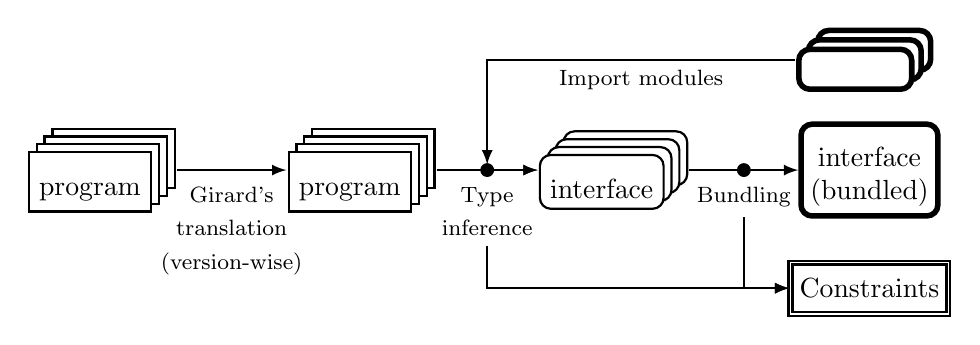
\begin{tikzpicture}[thick]
    \tikzset{vecArrow/.style={thick, decoration={markings,mark=at position
    1 with {\arrow[semithick]{open triangle 60}}},
    double distance=1.4pt, shorten >= 5.5pt,
    preaction = {decorate},
    postaction = {draw,line width=1.4pt, white,shorten >= 4.5pt}}};
    \tikzset{innerWhite/.style={semithick, white,line width=1.4pt, shorten >= 4.5pt}};
    \tikzset{Package/.style={rectangle, fill=cyan!10, text centered, rounded corners, minimum width=1.9cm, minimum height=0.65cm}};
    \tikzset{App/.style={rectangle, text centered, minimum width=1.2cm, minimum height=0.65cm}};

    \newlength\mywidth
    \newlength\myheight
    \newlength\tempdimen
    
    \newcommand\getdimensions[1]{
        \pgfextractx{\mywidth}{\pgfpointanchor{#1}{east}}
        \pgfextractx{\tempdimen}{\pgfpointanchor{#1}{west}}
        \addtolength{\mywidth}{-\tempdimen}
        \pgfextracty{\myheight}{\pgfpointanchor{#1}{north}}
        \pgfextracty{\tempdimen}{\pgfpointanchor{#1}{south}}
        \addtolength{\myheight}{-\tempdimen}
    }

    \tikzset{
      pics/stacked rectangles/.style n args={4}{
        code={
          \def\rectangleWidth{2cm}  % 長方形の幅を固定
          \def\rectangleHeight{1cm} % 長方形の高さを固定
          \pgfmathsetmacro\offsetY{(#1+1)*#2/2} % Yのオフセットを計算
          
          % 一時的なrect1を描画してサイズを取得
          \node[draw=none, align=center] (tempRect1) at (1*#2,1*#2-\offsetY) { #3 };
          
          % ここでtempRect1の寸法を取得
          \getdimensions{tempRect1}
          
          % 長方形を描画
          \foreach \i in {#1,...,2} {
            \node[draw, fill=white, minimum width=\mywidth, minimum height=\myheight] (rect\i) at (\i*#2,\i*#2-\offsetY) {};
          }

          % 一番前の長方形を描画
          \node[draw, fill=white, minimum width=\mywidth, minimum height=\myheight, align=center] (rect1) at (1*#2,1*#2-\offsetY) { #3 };
    
          % すべての長方形を囲む仮想的なノード
          \node[draw=none, inner sep=0pt, fit={(rect1.south west) (rect#1.north east)}, name=#4] {};
        }
      }
    }

    \tikzset{
      pics/stackedty rectangles/.style n args={4}{
        code={
          \def\rectangleWidth{2cm}  % 長方形の幅を固定
          \def\rectangleHeight{1cm} % 長方形の高さを固定
          \pgfmathsetmacro\offsetY{(#1+1)*#2/2} % Yのオフセットを計算
          
          % 一時的なrect1を描画してサイズを取得
          \node[draw=none, align=center] (tempRect1) at (1*#2,1*#2-\offsetY) { #3 };
          
          % ここでtempRect1の寸法を取得
          \getdimensions{tempRect1}
          
          % 長方形を描画
          \foreach \i in {#1,...,2} {
            \node[draw, fill=white, minimum width=\mywidth, minimum height=\myheight, rounded corners] (rect\i) at (\i*#2,\i*#2-\offsetY) {};
          }

          % 一番前の長方形を描画
          \node[draw, fill=white, minimum width=\mywidth, minimum height=\myheight, align=center, rounded corners] (rect1) at (1*#2,1*#2-\offsetY) { #3 };
    
          % すべての長方形を囲む仮想的なノード
          \node[draw=none, inner sep=0pt, fit={(rect1.south west) (rect#1.north east)}, name=#4] {};
        }
      }
    }


    \tikzset{
      pics/stackedtybundled rectangles/.style n args={4}{
        code={
          \def\rectangleWidth{2cm}  % 長方形の幅を固定
          \def\rectangleHeight{1cm} % 長方形の高さを固定
          \pgfmathsetmacro\offsetY{(#1+1)*#2/2} % Yのオフセットを計算
          
          % 一時的なrect1を描画してサイズを取得
          \node[draw=none, align=center] (tempRect1) at (1*#2,1*#2-\offsetY) { #3 };
          
          % ここでtempRect1の寸法を取得
          \getdimensions{tempRect1}
          
          % 長方形を描画
          \foreach \i in {#1,...,2} {
            \node[draw, fill=white, minimum width=\mywidth, minimum height=\myheight, rounded corners, line width=2pt] (rect\i) at (\i*#2,\i*#2-\offsetY) {};
          }

          % 一番前の長方形を描画
          \node[draw, fill=white, minimum width=\mywidth, minimum height=\myheight, align=center, rounded corners, line width=2pt] (rect1) at (1*#2,1*#2-\offsetY) { #3 };
    
          % すべての長方形を囲む仮想的なノード
          \node[draw=none, inner sep=0pt, fit={(rect1.south west) (rect#1.north east)}, name=#4] {};
        }
      }
    }

    \pic at (0,0) {stacked rectangles={4}{0.1cm}{\mylang{}\\program}{vl1}};
    % \node[draw,App, align=center] at (3.0,0) (vlmini1) {\vlmini{}\\($V_{M_i}$)};
    \pic at (3.3,0) {stacked rectangles={4}{0.1cm}{\vlmini{}\\program}{vlmini1}};
    % \node[draw,App, align=center] at (6.0,0) (vlmini2) {\vlmini{}\\interface};
    \pic at (6.5,0) {stackedty rectangles={4}{0.1cm}{\vlmini{}\\interface}{vlmini2}};
    \pic at (9.7,1.4) {stackedtybundled rectangles={3}{0.12cm}{\vphantom{b}\hspace{3em}}{vlmini4}};
    \node[draw,App, align=center, rounded corners, line width=2pt] at (10,0) (vlmini3) {\vlmini{}\\interface\\(bundled)};
    % \node[draw,App, align=center, rounded corners, line width=2pt, minimum width=1.62cm, minimum height=0.5cm] at (10,1.4) (vlmini4) {};
    \coordinate (topofinference) at ($(vlmini1.east)!0.5!(vlmini2.west)$);
    \coordinate (botofinference) at ($(vlmini1.east)!0.5!(vlmini2.west) + (0, -1.75)$);
    \coordinate (topofbundling) at ($(vlmini2.east)!0.5!(vlmini3.west)$);
    \coordinate (botofbundling) at ($(vlmini2.east)!0.5!(vlmini3.west) + (0, -1.75)$);
    % \node[draw,App,double,align=center] at (botofinference) (vdep) {\footnotesize{Variable}\\\footnotesize{dependency}};
    % \node[draw,App,double,align=center] at (botofbundling) (ldep) {\footnotesize{Label}\\\footnotesize{dependency}};
    \node[draw,App,double] at (10,-1.5) (constraints) {Constraints};
    \fill (topofinference) circle (2.5pt);
    \fill (topofbundling) circle (2.5pt);
    
    \draw[-latex] (vl1.east) to [yshift=-5]node[midway,below,align=center] {\footnotesize{Girard's}\\\footnotesize{translation}\\\footnotesize{(version-wise)}} (vlmini1.west);
    \draw[-latex] (vlmini1.east) to node[midway,below] {} (vlmini2.west);
    \draw[-latex] (vlmini1.east) to [yshift=-5]node[midway,below,align=center] (inference){\footnotesize{Type}\\\footnotesize{inference}} (vlmini2.west);
    \draw[-latex] (vlmini2.east) to [yshift=-5]node[midway,below,align=center] (bundling) {\footnotesize{Bundling}} (vlmini3.west);
    \draw[-latex] (vlmini4.west) -| node[near start,below,align=center] {\footnotesize{Import modules}} ([yshift=2]topofinference);
    \draw[-latex] (inference.south) |- (constraints.west);
    \draw[-latex] (bundling.south) |- (constraints.west);
    % \draw[-latex] (inference.south) -- (vdep.north);
    % \draw[-latex] (bundling.south) -- (ldep.north);
\end{tikzpicture}
\caption{The translation phases for a single module with multiple versions.}
\label{fig:translationoverview}
\end{figure}
The entire translation consists of three parts: (1) \emph{Girard's translation}, (2) an \emph{algorithmic type inference}, and (3) \emph{bundling}.
Figure \ref{fig:translationoverview} shows the translation process of a single module. First, through Girard's translation, each version of the \mylang{} program undergoes a version-wise translation into the \vlmini{} program. 
Second, the type inference synthesizes types and constraints for top-level symbols. Variables imported from external modules reference the bundled interface generated in the subsequent step.
Finally, to make the external variables act as multi-version expressions, bundling consolidates each version's interface into one \vlmini{} interface.
These translations are carried out in order from downstream of the dependency tree.
By resolving all constraints up to the main module, the appropriate version for every external variable is determined.

It is essential to note that the translations focus on generating constraints for dispatching external variables into version-specific code. While implementing versioned records in \corelang{} presents challenges, such as handling many version labels and their code clones, our method is a constraint-based approach in \vlmini{} that enables static inference of version labels without their explicit declaration.

In the context of coeffect languages, constraint generation in \mylang{} can be seen as the automatic generation of type declarations paired with resource constraints.
Granule\cite{Orchard:2019:Granule} can handle various resources as coeffects, but it requires type declarations to indicate resource constraints. \mylang{} restricts its resources solely to the version label set. This specialization enables the automatic collection of version information from external sources outside the codebase.

\subsection{An Intermediate Language, \vlmini{}}
% \vspace{-1\baselineskip}
\subsubsection{Syntax of \vlmini{}}
\begin{figure}[tb]
    \hrule
    \medskip
    \begin{minipage}{.9\textwidth}
        \textbf{\vlmini{} syntax (w/o data constructors and version control terms)}
    \end{minipage}
    \begin{minipage}{\textwidth}
        \vspace{-.8\baselineskip}
        \begin{minipage}{.475\textwidth}
          \begin{align*}
            t & ::= n \mid x \mid \app{t_1}{t_2} \mid \lam{p}{t} \mid \pr{t} \tag{terms}\\
            p & ::= x \mid [x] \tag{patterns}\\
            A, B & ::= \inttype{} \mid \alpha \mid \ftype{A}{B} \mid \vertype{r}{A} \tag{types}\\
            \kappa & ::= \typekind{} \mid \labelskind{} \tag{kinds}
          \end{align*}
        \end{minipage}
        \begin{minipage}{.475\textwidth}
          \begin{align*}
            \Gamma & ::= \emptyset \mid \Gamma, x:A \mid \Gamma, x:\verctype{A}{r} \tag{contexts}\\
            \Sigma & ::= \emptyset \mid \Sigma, \alpha:\kappa \tag{type variable kinds}\\
            R      & ::= - \mid r \tag{resource contexts}\\
          \end{align*}
        \end{minipage}
    \end{minipage}
    \begin{minipage}{.9\textwidth}
        \medskip\textbf{Extended with data constructors}
    \end{minipage}
    \begin{minipage}{\textwidth}
        \vspace{-.5\baselineskip}
        \begin{minipage}{.52\textwidth}
          \begin{align*}
            t & ::= \ldots \mid C\,\overline{t_i} \mid \caseof{t}{\overline{p_i \mapsto t_i}}\tag{terms}\\
            p & ::= \ldots \mid C\,\overline{p_i} \tag{patterns}\\
            C & ::= (,) \mid [,] \tag{constructors}
          \end{align*}
        \end{minipage}
        \begin{minipage}{.44\textwidth}
          \begin{align*}
            A, B & ::= ... \mid K \overline{A_i} \tag{types}\\
            K    & ::= (,) \mid [,] \tag{type constructors}\\
          \end{align*}
        \end{minipage}
    \end{minipage}
    \begin{minipage}{.9\textwidth}
        \medskip\textbf{Extended with version control terms}
    \end{minipage}
    \begin{minipage}{\textwidth}
        \vspace{-.5\baselineskip}
        \begin{minipage}{\textwidth}
          \begin{align*}
            t & ::= \ldots \mid \verof{\{\overline{M_i=V_i}\}}{t} \mid \unver{t}\hspace{6em}\tag{terms}
          \end{align*}
        \end{minipage}
    \end{minipage}
    \begin{minipage}{.9\textwidth}
        \medskip\textbf{\vlmini{} constraints}
    \end{minipage}
    \begin{minipage}{\textwidth}
      \vspace{-.5\baselineskip}
      \begin{align*}
        \mathcal{C} & ::= \underbrace{\top \mid \mathcal{C}_1 \land \mathcal{C}_2 \mid \mathcal{C}_1 \lor \mathcal{C}_2}_{\substack{\text{propositional}\\\text{formulae}}} \mid \underbrace{\vphantom{\mid}\alpha \preceq \alpha'}_{\substack{\text{variable}\\\text{dependencies}}} \mid \underbrace{\vphantom{\mid}\alpha \preceq \mathcal{D}}_{\substack{\text{label}\\\text{dependencies}}}\tag{dependency 
 constraints}\\
        \mathcal{D} & ::= \cs{\overline{M_i = V_i}} \tag{dependent labels}\\
        \Theta      & ::= \top \mid \Theta_1 \land \Theta_2 \mid \{A \sim B\} \tag{type constraints}
      \end{align*}
    \end{minipage}
  % \begin{align*}
  %   t & ::= n \mid x \mid \app{t_1}{t_2} \mid \lam{p}{t} \mid \pr{t} \mid C\,\overline{t_i} \mid \caseof{t}{\overline{p_i \mapsto t_i}}\tag{terms}\\
  %   p & ::= n \mid x \mid \_ \mid [p] \mid C\,\overline{p_i} \tag{patterns}\\
  %   C & ::= (,) \mid [,] \tag{constructors}\\
  %   A, B & ::= \inttype{} \mid K \overline{A_i} \mid \bgr{\alpha} \mid \ftype{A}{B} \mid \vertype{r}{A} \tag{types}\\
  %   K    & ::= (,) \mid [,] \tag{type constructors}\\
  %   \kappa & ::= \typekind{} \mid \labelskind{} \tag{kinds}\\
  %   \Gamma & ::= \emptyset \mid \Gamma, x:A \mid \Gamma, x:\verctype{A}{r} \tag{contexts}\\
  %   \Sigma & ::= \emptyset \mid \Sigma, \alpha:\kappa \tag{type variable kinds}\\
  %   R      & ::= - \mid r \tag{resource contexts}\\
  %   \mathcal{C} & ::= \top \mid \mathcal{C}_1 \land \mathcal{C}_2 \mid \mathcal{C}_1 \lor \mathcal{C}_2 \mid \underbrace{\vphantom{\mid}\alpha \preceq \alpha'}_{\textnormal{variable dependencies}} \mid \underbrace{\vphantom{\mid}\alpha \preceq L}_{\textnormal{label dependencies}}\tag{constraints}\\
  %   L & ::= \cs{\overline{M_i \mapsto V_i}} \tag{dependent labels}
  % \end{align*}
  \medskip
  \hrule
  \caption{The syntax of \vlmini{}.}
  \label{syntax:vlmini}
\end{figure}
Figure \ref{syntax:vlmini} shows the syntax of \vlmini{}.
\vlmini{} encompasses all the terms in \corelang{} except for versioned records $\nvval{l_i=t_i}$, intermediate term $\ivval{\overline{l_i=t_i}}{l_k}$, and extractions $t.l_k$. As a result, its terms are analogous to those in \lrpcf{}\cite{brunel_core_2014} and GrMini\cite{Orchard:2019:Granule}. However, \vlmini{} is specialized to treat version resources as coeffects.
We also introduce data constructors by introduction $C\,t_1,...,t_n$ and elimination $\caseof{t}{\overline{p_i \mapsto t_i}}$ for lists and pairs, and version control terms \unver{t} and \verof{\{\overline{M_i=V_i}\}}{t}. 
Here, contextual-let in \corelang{} is a syntax sugar of lambda abstraction applied to a promoted pattern.
\begin{align*}
\clet{x}{t_1}{t_2} \triangleq \app{(\lam{\pr{x}}{t_2})}{t_1}
\end{align*}

Types, version labels, and version resources are almost the same as \corelang{}.
Type constructors are also added to the type in response to the \vlmini{} term having a data constructor.
The remaining difference from \corelang{} is type variables $\alpha$. Since \vlmini{} is a monomorphic language, type variables act as unification variables; type variables are introduced during the type inference and are expected to be either concrete types or a set of version labels as a result of constraint resolution.
To distinguish those two kinds of type variables, we introduce kinds $\kappa$.
The kind \labelskind{} is given to type variables that can take a set of labels $\{\overline{l_i}\}$ and is used to distinguish them from those of kind \typekind{} during algorithmic type inference.

% \vspace{-1\baselineskip}
\subsubsection{Constraints}
% \subsection{Constraints}

In many trajectory optimization problems, there are constraints on the trajectory. It should be noted that these are different than a simple bound on the system input or state. In walking robots, common constraints are: 

\begin{itemize}
	\item reaction forces in friction cone
	\item robot above the ground
	\item robot moving forward
	\item foot hits ground from above... 
\end{itemize}

The most important thing to notice about constraints is that they must also be consistent and smooth. It isn't enough to say ``The lowest point of the foot during the step must be above the ground'' because this will pass data from a different grid-point on each function call. Rather, you need to say ``Every point of the foot trajectory must be above the ground'' (or use some very fancy smoothing in your maximization function). All rules that apply to objective functions regarding smoothness and consistency, also should be applied to calculations of constraints.

\par It is also important to minimize the number of unused constraints, provided that the problem remains smooth and consistent. One way to do this is to leave all of the constraints active, and then as you refine the solution, remove the constraints that are not being actively used. At the end of each run, check to make sure that the solution still satisfies the constraints.


The lower part of Figure \ref{syntax:vlmini} shows constraints generated through bundling and type inference.
Dependency constraints comprise \emph{variable dependencies} and \emph{label dependencies} in addition to propositional formulae.
Variable dependencies $\alpha \sqsubseteq \alpha'$ require that if a version label for $\alpha'$ expects a specific version for a module, then $\alpha$ also expects the same version.
Similarly, label dependencies $\alpha \preceq \cs{\overline{M_i = V_i}}$ require that a version label expected for $\alpha$ must be $V_i$ for $M_i$. For example, assuming that versions $1.0.0$ and $2.0.0$ exist for both modules \mn{A} and \mn{B}, the minimal upper bound set of version labels satisfying $\alpha \preceq \cs{\mn{A}\mapsto 1.0.0}$ is $\alpha = \{\{\mn{A}=1.0.0,\mn{B}=1.0.0\},\{\mn{A}=1.0.0,\mn{B}=2.0.0\}\}$. If the constraint resolution is successful, $\alpha$ will be specialized with either of two labels.
$\Theta$ is a set of type equations resolved by the type unification.

\subsection{Girard's Translation for \vlmini{}}
\label{sec:VLMini}
We extend Girard's translation between \mylang{} (lambda calculus) to \vlmini{} following Orchard's approach~\cite{Orchard:2019:Granule}.
\begin{align*}
\llbracket n \rrbracket \equiv n \qquad
\llbracket x \rrbracket \equiv x \qquad
\llbracket \lam{x}{t} \rrbracket \equiv \lam{[x]}{\llbracket t \rrbracket} \qquad
\llbracket t\ s\rrbracket \equiv \llbracket t\rrbracket\ [ \llbracket s \rrbracket ]
\end{align*}

The translation replaces lambda abstractions and function applications of \mylang{} by lambda abstraction with promoted pattern and promotion of \vlmini{}, respectively. From the aspect of types, this translation replaces all occurrences of $\ftype{A}{B}$ with $\ftype{\vertype{r}{A}}{B}$ with a version resource $r$.
This translation inserts a syntactic annotation $[*]$ at each location where a version resource needs to be addressed. Subsequent type inference will compute the resource at the specified location and produce constraints to ensure version consistency at that point.

The original Girard's translation~\cite{girardlinear1987} is well-known as a translation between the simply-typed $\lambda $-calculus and an intuitionistic linear calculus. The approach involves replacing every intuitionistic arrow $A \rightarrow B$ with $!A \multimap B$, and subsequently unboxing via let-in abstraction and promoting during application \cite{Orchard:2019:Granule}.













\subsection{Bundling}
\label{sec:bundling}
Bundling produces an interface encompassing types and versions from every module version, allowing top-level symbols to act as multi-version expressions. During this process, bundling reviews interfaces from across module versions, identifies symbols with the same names and types after removing $\square_r$ using Girard's transformation, and treats them as multiple versions of a singular symbol (also discussed in Section \ref{sec:typeincompatibilities}). In a constraint-based approach, bundling integrates label dependencies derived from module versions, ensuring they align with the version information in the typing rule for versioned records of \corelang{}.

For example, assuming that the $\mathit{id}$ that takes an \inttype{} value as an argument is available in version 1.0.0 and 2.0.0 of \mn{M} as follows:
\begin{align*}
\mathit{id} &: \vertype{\alpha_1}{(\ftype{\vertype{\alpha_2}{\inttype}}{\inttype})}\ |\ \mathcal{C}_1 \tag{\textnormal{version 1.0.0}}\\
\mathit{id} &: \vertype{\beta_1}{(\ftype{\vertype{\beta_2}{\inttype}}{\inttype})}\ |\ \mathcal{C}_2 \tag{\textnormal{version 2.0.0}}
\end{align*}
where $\alpha_1$ and $\alpha_2$ are version resource variables given from type inference. They capture the version resources of $\mathit{id}$ and its argument value in version 1.0.0. $\mathcal{C}_1$ is the constraints that resource variables of version 1.0.0 will satisfy. Likewise for $\beta_1$, $\beta_2$, and $\mathcal{C}_2$.
Since the types of $\mathit{id}$ in both versions become $\ftype{\inttype}{\inttype}$ via Girard's translation, they can be bundled as follows:
\begin{align*}
\mathit{id} : \vertype{\gamma_1}{(\ftype{\vertype{\gamma_2}{\textsf{Int}}}{\textsf{Int}})}\ |\
\mathcal{C}_1 \land \mathcal{C}_2 \land \Bigl(\ 
     &(\gamma_1 \preceq \cs{\mn{M} = 1.0.0} \land \gamma_1 \preceq \alpha_1 \land \gamma_2 \preceq \alpha_2)\\
\lor\ &(\gamma_1 \preceq \cs{\mn{M} = 2.0.0} \land \gamma_1 \preceq \beta_1 \land \gamma_2 \preceq \beta_2)\ \Bigr)
\end{align*}
where $\gamma_1$ and $\gamma_2$ are introduced by this conversion for the bundled $id$ interface, with label and variable dependencies that they will satisfy.
$\gamma_1$ captures the version resource of the bundled $\mathit{id}$. The generated label dependencies $\gamma_1 \preceq \cs{\mn{M} = 1.0.0}$ and $\gamma_1 \preceq \cs{\mn{M} = 2.0.0}$ indicate that $\mathit{id}$ is available in either version 1.0.0 or 2.0.0 of \mn{M}.
These label dependencies are exclusively\footnote{In the type checking rules for $\verof{l}{t}$, type inference exceptionally generates label dependencies. Please see Appendix \ref{appendix:vlmini_version_control_terms}} generated during bundling.
The other new variable dependencies indicate that the $\mathit{id}$ bundled interface depends on one of the two version interfaces. The dependency is made apparent by pairing the new resource variables with their respective version resource variable for each version.
These constraints are retained globally, and the type definition of the bundled interface is used for type-checking modules importing $\mathit{id}$. 

 
\section{Building blocks for approximate inference algorithms} \label{sec:inference}

This section first describes a set of building blocks for approximate inference algorithms
that are based on the generative model of Section~\ref{sec:model}.
We then describe how to combine these components into a scene graph inference algorithm
that we evaluate in Section~\ref{sec:experiments}.

\paragraph{Trained object detectors}
It is possible to infer the types of objects in the scene ($\mathbf{c}$) via Bayesian inference in the generative model
(see supplement for an example that infers $\mathbf{c}$ as well as $N$ in a scene with a fully occluded object, via Bayesian inference).
However, for scenes where objects are not fully or nearly-fully occluded,
and where object types have dissimilar appearance,
it is possible to train fast object detectors
that produce an accurate point estimate of $\mathbf{c}$ given an RGB image.

\paragraph{Trained pose estimators}
In scenes without full or nearly-full occlusion, it is also possible to employ trained pose estimation methods~\citep{wang2019densefusion} to give independent estimates of the 6DoF pose of each object instance in the image.
However, inferring pose is more challenging than inferring $\mathbf{c}$,
and occlusion, self-occlusion, and symmetries can introduce significant pose uncertainty.
Therefore, we only use trained pose estimators (e.g. \citep{wang2019densefusion}) to (optionally) \emph{initialize} the poses of objects before Bayesian inference in the generative model, using the building blocks below.

\paragraph{Data-driven Metropolis-Hastings kernels on object pose}
We employ Metropolis-Hastings (MH) kernels, parametrized by choice of object $i \in \{1, \ldots, N\}$, that
take as input a scene graph $\mathcal{G}$,
propose new values ($\theta_{v_i}'$) for the scene graph parameters of object $i$,
construct a new proposed scene graph $\mathcal{G'}$,
and then accept or reject the move from $\mathcal{G}$ to $\mathcal{G'}$ based on 
the MH rule.
For objects $v$ whose parent is the world frame ($(r, v) \in E$), we use a data-driven proposal distribution centered on an estimate ($\hat{\mathbf{x}}_v$) of the 6DoF object pose obtained with ICP 
(a spherical normal distribution concentrated around the estimated position,
and a vMF distribution concentrated around the estimated orientation).
We also use kernels with random-walk proposals centered on the current pose.
For objects whose parent is another object ($(u, v) \in E$ for $u \ne r$),
we use a random-walk proposal on parameters $(a_{v_i}$, $b_{v_i}$, $z_{v_i})$.
Note that when the pose of an object is changed in the proposed graph $\mathcal{G'}$,
the pose of any descendant objects is also changed.\footnote{%
It is possible to construct an involutive MCMC kernel that does not change the poses of descendant objects.}
Each of these MH kernels is invariant with respect to $p(G, \bm\theta | \mathbf{c}, \mathbf{Y})$.

\begin{figure}[t]
	\centering
	\includegraphics[width=0.8\textwidth]{imgs/scene-graphs-structure-transition.pdf}
	\caption{A reversible transition between scene graph structure $G$ and scene graph structure $G'$.}
	\label{fig:scene-graph-structure-change}
\end{figure}


\paragraph{Involutive MCMC kernel on scene graph structure}
To infer the scene graph structure $G$, we employ a family of involutive MCMC kernels~\citep{cusumano2020automating} that
propose a new graph structure $G'$ while keeping the poses ($\mathbf{x}_v$) of all objects fixed.
The kernel takes a graph structure $G$ and proposes a new graph structure $G'$ (Figure~\ref{fig:scene-graph-structure-change}) by:
(i) randomly sampling a node $v \in V \setminus \{r\}$ to `sever' from the tree,
(ii) randomly choosing a node $u \in V \setminus \{v\}$ that is not a descendant of the severed node on which to graft $v$,
(iii) forming a new directed graph $G'$ over vertices $V$ by grafting $v$ to $u$; by Lemma~O.7.1 the resulting graph $G'$ is also a tree.
Note that there is an involution $g$ on the set of all pairs $(G, v, u)$ satisfying the above constraints.
That is, if
$(G', v', u') = g(G, v, u)$
then
$(G, v, u) = g(G', v', u')$.
(This implies, for example, that $u'$ is the parent of $v$ in $G$.)
Note that this set of transitions is capable of changing the parent vertex of an object to a different parent object,
changing the parent vertex of an object from the root (world frame) to any other object,
or changing the parent vertex from another object to the root, depending on the random choice of $v$ and $u$.
We compute new values for parameters ($\theta_v$) for the severed node $v$ and possibly other vertices such that the poses of all vertices are unchanged.
See supplement for the full kernel and a proof that it is invariant w.r.t. $p(G, \bm\theta | \mathbf{c}, \mathbf{Y})$.

\paragraph{Approximately Rao--Blackwellizing object shape via pseudo-marginal MCMC}
The acceptance probability expressions for our involutive MCMC and MH kernels targeting $p(G, \bm\theta | \mathbf{c}, \mathbf{Y})$ include factors of the form $p(\mathbf{Y} | \mathbf{c}, G, \bm{\theta})$, which is an intractable sum over the latent object models:
$p(\mathbf{Y} | \mathbf{c}, G, \bm{\theta}) = \sum_{\mathbf{O}^{(1:M)}} p(\mathbf{O}^{(1:M)}) p(\mathbf{Y} | \mathbf{O}^{(1:M)}, \mathbf{c}, G, \bm{\theta})$.
To overcome this challenge, we employ a pseudo-marginal MCMC approach \citep{andrieu2009pseudo} that uses unbiased estimates of
$p(\mathbf{Y} | \mathbf{c}, G, \bm{\theta})$
obtained via likelihood weighting (that is, sampling several times from $p(\mathbf{O}^{(1:M)})$ and averaging the resulting $p(\mathbf{Y} | \mathbf{O}^{(1:M)}, \mathbf{c}, G, \bm\theta$)).
The resulting MCMC kernels are invariant with respect to an extended target distribution of which $p(G, \bm\theta | \mathbf{c}, \mathbf{Y})$ is a marginal (see supplement for details). % \ref{sec:pseudo-marginal} 
We implemented an optimization where we sampled 5 values for $\mathbf{O}^{(1:M)}$ and used these samples within every estimate of $p(\mathbf{Y} | \mathbf{c}, G, \bm\theta)$ instead of sampling new values for each estimate.
Because our learned shape priors did not have significant exterior shape uncertainty,
this optimization did not negatively impact the results.

\paragraph{Scene graph inference and implementation}
The end-to-end scene graph inference algorithm has three stages.
First, we obtain $\mathbf{c}$ from either an object detector or because it is given as part of the task (this is the case in our experiments; see Section~\ref{sec:experiments} for details).
Second, we obtain initial estimates $\hat{\mathbf{x}}_v$ of 6DoF object poses $\mathbf{x}_v$ for all object vertices $v$ via maximum-a-posteriori (MAP) inference in a restricted variant of the generative model with graph structure $G$ fixed to $G_0$ (so there are no edges between object vertices).
This MAP inference stage uses the data-driven Metropolis-Hastings kernels on poses, and (optionally) trained pose estimators (see Section~\ref{sec:experiments} for the details, which differ between experiments).
Third, we use the estimated poses to initialize an MCMC algorithm targeting $p(G, \bm{\theta} | \mathbf{c}, \mathbf{Y})$ with state $G \gets G_0$ and $\theta_v \gets \hat{\mathbf{x}}_v$ for each $v \in V \setminus \{r\}$.
The Markov chain is a cycle of the involutive MCMC kernel described above with a mixture of the Metropolis-Hastings kernels described above, uniformly mixed over objects.
We wrote the probabilistic program of Figure~\ref{fig:model} in Gen's built-in modeling language.
We implemented the data-driven and involutive MCMC kernels, and pseudo-marginal likelihood,
and integrated all components together, using Gen's programmable inference support.
Our code is available at \url{https://github.com/probcomp/ThreeDP3}.

 
\section{Implementation: Ring Abstraction}
\label{sec:implement}
\subsection{Distributed \mbox{$G_t$} in QMC Solver}
\label{distributedG4}
Before introducing the communication phase of the ring abstraction layer,
it is important to understand how the authors distributed the large device array $G_t$ across MPI ranks.
%
Original $G_t$ was compared, and $G^d_t$ versions were distributed
(Figure~\ref{fig:compare_original_distributed_g4}). 


In the original $G_t$ implementation, the measurements---which were computed by matrix-matrix multiplication---are distributed statically and independently over the MPI ranks to avoid
inter-node communications. Each MPI rank keeps its partial copy of $G_{t,i}$ to accumulate 
measurements within a rank, where $i$ is the rank index. 
After all the measurements are finished, a reduction step is 
taken to accumulate $G_{t,i}$ across all MPI ranks into a final and complete
$G_t$ in the root MPI rank. The size of the $G_{t,i}$ in each rank is 
the same size as the final and complete $G_t$. 

With the distributed $G^d_t$ implementation, this large device array 
$G_t$ was evenly partitioned across all MPI ranks; each portion of it is local to each MPI rank.
%
Instead of keeping its partial copy of $G_t$, 
each rank now keeps an instance of $G^d_{t,i}$ to accumulate measurements 
of a portion or sub-slice of the final and complete $G_t$, where the notation
$d$ in $G^d_t$  refers to the distributed version, and $i$ means the $i$-th rank.
%
The $G^d_{t,i}$ size in each rank is 
reduced to $1/p$ of the size of the final and complete $G_t$, comparing the same configuration 
in original $G_t$ implementation, where $p$ is the number of MPI ranks used. 
%
For example, in Figure~\ref{fig:distributed_g4}, there are four ranks, and rank $i$
now only keeps $G^d_{t,i}$, which is one-fourth the size of the original $G_t$ array size.
% and contains values indexing from range of $[0, ..., N/4)$ in original $G_t$ array where $N$ is the 
% number of entries in  $G_t$  when viewed as a one-dimensional array.

To compute the final and complete $G^d_{t,i}$ for the distributed $G^d_t$ implementation, 
each rank must see every $G_{\sigma,i}$ from all ranks. 
%
In other words, each rank must broadcast the
locally generated $G_{\sigma,i}$ to the remainder of the other ranks at every measurement step. 
%
To efficiently perform this ``all-to-all'' broadcast, a ring abstraction layer was built (Section. \ref{section:ring_algorithm}), which circulates
all $G_{\sigma,i}$ across all ranks.

% over high-speed GPUs interconnect (GPUDirect RDMA) to facilitate the communication phase.

% \begin{figure}
% \centering
% \subfloat[Original $G_t$ implementation.]
%     {\includegraphics[width=\columnwidth]{original_g4.pdf}}\label{fig:original_g4}

% \subfloat[Distributed $G_t$ implementation.]
%     {\includegraphics[width=0.99\columnwidth]{distributed_g4.pdf} \label{fig:distributed_g4}}

% \caption{Comparison of the original $G_t$ vs. the distributed $G^d_t$ implementation. Each rank contains one GPU resource.}
% \label{fig:compare_original_distributed_g4} 
% \end{figure} 

\begin{figure}
\centering
     \begin{subfigure}[b]{\columnwidth}
         \centering
         \includegraphics[width=\textwidth]{images/original_g4.pdf}
         \caption{Original $G_t$ implementation.}
         \label{fig:original_g4}
     \end{subfigure}
     
    \begin{subfigure}[b]{\columnwidth}
         \centering
         \includegraphics[width=\textwidth]{images/distributed_g4.pdf}
         \caption{Distributed $G_t$ implementation.}
         \label{fig:distributed_g4}
     \end{subfigure}
     
\caption{Comparison of the original $G_t$ vs. the distributed $G^d_t$ implementation. Each rank contains one GPU resource.}
\label{fig:compare_original_distributed_g4}
\end{figure}

\subsection{Pipeline Ring Algorithm}
\label{section:ring_algorithm}
A pipeline ring algorithm was implemented that broadcasts the $G_{\sigma}$ 
array circularly during every measurement. 
%
The algorithm (Algorithm \ref{alg:ring_algorithm_code}) is 
visualized in Figure~\ref{fig:ring_algorithm_figure}.

\begin{algorithm}
\SetAlgoLined
    generateGSigma(gSigmaBuf)\; \label{lst:line:generateG2}
    updateG4(gSigmaBuf)\;       \label{lst:line:updateG4}
    %\texttt{\\}
    {$i\leftarrow 0$}\;         \label{lst:line:initStart}
    {$myRank \leftarrow worldRank$}\;          \label{lst:line:initRankId}
    {$ringSize \leftarrow mpiWorldSize$}\;      \label{lst:line:initRingSize}
    {$leftRank \leftarrow (myRank - 1 + ringSize) \: \% \: ringSize $}\;
    {$rightRank \leftarrow (myRank + 1 + ringSize) \: \% \: ringSize $}\;
    sendBuf.swap(gSigmaBuf)\;           \label{lst:line:initEnd}
    \While{$i< ringSize$}{
        MPI\_Irecv(recvBuf, source=leftRank, tag = recvTag, recvRequest)\; \label{lst:line:Irecv}
        MPI\_Isend(sendBuf, source=rightRank, tag = sendTag, sendRequest)\; \label{lst:line:Isend}
        MPI\_Wait(recvRequest)\;        \label{lst:line:recevBuffWait}
        
        updateG4(recvBuf)\;             \label{lst:line:updateG4_loop}
        
        MPI\_Wait(sendRequest)\;        \label{lst:line:sendBuffWait}
        
        sendBuf.swap(recvBuf)\;         \label{lst:line:swapBuff}
        i++\;
    }
\caption{Pipeline ring algorithm}
\label{alg:ring_algorithm_code}
\end{algorithm}

\begin{figure}
	\centering
	\includegraphics[width=\columnwidth, trim=0 5cm 0 0, clip]{images/ring_algorithm.pdf}
	\caption{Workflow of ring algorithm per iteration. }
	\label{fig:ring_algorithm_figure}
\end{figure}

At the start of every new measurement, a single-particle Green's function $G_{\sigma}$
 (Line~\ref{lst:line:generateG2}) is generated 
and then used to update $G^d_{t,i}$ (Line~\ref{lst:line:updateG4})
via the formula in Eq.~(\ref{eq:G4}).
%
% Different from original method that performs 
% full matrix-matrix multiplication (Equation~(\ref{eq:G4})), the current ring algorithm only performs partial
% matrix-matrix multiplication that contributes to $G^d_{t,i}$, a subslice of the final and complete $G_t$.
%
Between Lines \ref{lst:line:initStart} to \ref{lst:line:initEnd}, the algorithm 
initializes the indices
of left and right neighbors and prepares the sending message buffer from the
previously generated $G_{\sigma}$ buffer. 
%
The processes are organized as a ring so that the first and last rank are considered to be neighbors to each other. 
%
A \textit{swap} operation is used to avoid unnecessary memory copies for \textit{sendBuf} preparation.
%
A walker-accumulator thread allocates an additional \textit{recvBuf} buffer of the same size 
as \textit{gSigmaBuf} to hold incoming 
\textit{gSigmaBuf} buffer from \textit{leftRank}. 

The \textit{while} loop is the core part of the pipeline ring algorithm. 
%
For every iteration, each thread in a rank 
receives a $G_{\sigma}$ buffer from its left neighbor rank and sends a $G_{\sigma}$ buffer to its right neighbor rank. 
A synchronization step (Line~\ref{lst:line:recevBuffWait}) is performed
afterward to ensure that each rank receives a new buffer to update the 
local $G^d_{t,i}$ (Line~\ref{lst:line:updateG4_loop}). 
%
Another synchronization step
follows to ensure that all send requests are finalized 
(Line~\ref{lst:line:sendBuffWait}). Lastly, another \textit{swap} operation is used to exchange
content pointers between \textit{sendBuf} and \textit{recvBuf} to avoid unnecessary memory copy and prepare
for the next iteration of communication.
%
In the multi-threaded version (Section~\ref{subsec:multi-thread}), the thread of index, \textit{i}, only communicates with
	threads of index, \textit{i}, in neighbor ranks, and each thread allocates two buffers: \textit{sendBuff} and \textit{recvBuff}.

The \textit{while} loop will be terminated after $\mbox{\textit{ringSize}} - 1$ steps. By that time, 
each locally generated $G_{\sigma,i}$ will have traveled across all MPI ranks and
updated $G^d_{t,i}$ in all ranks. Eventually, each $G_{\sigma,i}$ reaches
to the left neighbor of its birth rank. For example, $G_{\sigma,0}$ generated from rank $0$ will end 
in last rank in the ring communicator.

Additionally, if the $G_t$ is too large to be stored in one node, 
it is optional to accumulate all $G^d_{t,i}$
at the end of all measurements. 
%
Instead, a parallel write into the file system could be taken.

\subsubsection{Sub-Ring Optimization.}

A sub-ring optimization strategy is further proposed to reduce message communication
times if the large device array $G_t$ can fit in fewer devices. 
%
The sub-ring algorithm is visualized in Figure~\ref{fig:subring_algorithm_figure}.

For the ring algorithm (Section~\ref{section:ring_algorithm}), the size of the ring communicator
(\textit{mpiWorldSize}) is set to the same size of the global \mbox{\texttt{MPI\_COMM\_WORLD}}, and thus the size of $G_t$ is equally 
distributed across all MPI ranks.

However, to complete the update to $G^d_{t,i}$ in one measurement, 
one $G_{\sigma,i}$
must travel \textit{mpiWorldSize} ranks. In total, 
there are \textit{mpiWorldSize} numbers of $G_{\sigma,i}$
being sent and received concurrently in one measurement 
in the global
\mbox{\texttt{MPI\_COMM\_WORLD}} 
communicator. If the size of $G^d_{t,i}$ is relatively small per rank, then this will cause high communication overhead.

If $G_t$ can be distributed and fitted in fewer devices, then a shorter travel distance is required 
for $G_{\sigma,i}$, thus reducing the communication overhead. One reduction
step was performed at the end of all measurements to accumulate $G^d_{t,s_i}$, 
where $s_i$ means $i$-th rank on the $s$-th sub-ring.

At the beginning of MPI initialization, the global \mbox{\texttt{MPI\_COMM\_WORLD}} was partitioned  into several new sub-ring communicators by using \mbox{\texttt{MPI\_Comm\_split}}. 
% where each new communicator represents conceptually a subring. 
The new
communicator information was passed to the DCA++ concurrency class by substituting the original global 
\mbox{\texttt{MPI\_COMM\_WORLD}} with this new communicator. Now, only a few minor modifications
are needed to transform the ring algorithm (Algorithm~\ref{alg:ring_algorithm_code})
to sub-ring Algorithm~\ref{alg:sub_ring_algorithm}. In Line~\ref{lst:line:initRankId}, \textit{myRank} is 
initialized to \textit{subRingRank} instead of \textit{worldRank}, where 
\textit{subRingRank} is the rank index in the local sub-ring communicator. 
%
In Line~\ref{lst:line:initRingSize}, \textit{ringSize} is initialized to \textit{subRingSize}
instead of \textit{mpiWorldSize}, where \textit{subRingSize} is the
size of the new communicator.
%
The general ring algorithm is a special case for the sub-ring algorithm because the
\textit{subRingSize} of the general ring algorithm is equal to \textit{mpiWorldSize}, and
there is only one sub-ring group throughout all MPI ranks.


\LinesNumberedHidden
\begin{algorithm}
    {$\mbox{\textit{myRank}} \leftarrow \mbox{\textit{subRingRank}}$}\;         
    {$\mbox{\textit{ringSize}} \leftarrow \mbox{\textit{subRingSize}}$}\;      
\caption{Modified ring algorithm to support sub-ring communication}
\label{alg:sub_ring_algorithm}
\end{algorithm}


\begin{figure}
	\centering
	\includegraphics[width=\columnwidth, trim=0 5cm 0 0, clip]{images/subring_alg.pdf}
	\caption{Workflow of sub-ring algorithm per iteration. Every consecutive $S$ rank forms a sub-ring communicator, 
	and no communication occurs between sub-ring communicators until all measurements are finished. Here, $S$ is the number of ranks in a sub-ring.}
	\label{fig:subring_algorithm_figure}
\end{figure}

\subsubsection{Multi-Threaded Ring Communication.}
\label{subsec:multi-thread}
To take advantage of the multi-threaded QMC model already in DCA++, 
multi-threaded ring communication support was further implemented in the ring algorithm.
%
Figure~\ref{fig:dca_overview} shows that in the original DCA++ method,
each walker-accumulator
thread in a rank is independent of each other, and all the threads in a 
rank synchronize only after all rank-local measurements are finished.
%
Moreover, during every measurement, each walker-accumulator thread
generates its own thread-private $G_{\sigma, i}$ to update $G_t$. 
%

The multi-threaded ring algorithm now allows concurrent message exchange so that threads of same rank-local thread index exchange their thread-private $G_{\sigma, i}$. 
%
Conceptually, there are $k$ parallel and independent rings, where $k$ 
is number of threads per rank, because threads of the same local thread ID
form a closed ring. 
%
For example, a thread of index $0$ in rank $0$ will send its $G_\sigma$ to 
the thread of index $0$ in rank $1$ and receive another $G_\sigma$ from thread index of $0$ 
from last rank in the ring algorithm.
%

The only changes in the ring algorithm are offsetting the tag values 
(\texttt{recvTag} and \texttt{sendTag}) by the thread index value. For example,
Lines~\ref{lst:line:Irecv} and ~\ref{lst:line:Isend} from 
Algorithm~\ref{alg:ring_algorithm_code} are modified to Algorithm~\ref{alg:multi_threaded_ring}.

\LinesNumberedHidden
\begin{algorithm}
        MPI\_Irecv(recvBuf, source=leftRank, tag = recvTag + threadId, recvRequest)\; 
        MPI\_Isend(sendBuf, source=rightRank, tag = sendTag + threadId, sendRequest)\;
\caption{Modified ring algorithm to support multi-threaded ring}
\label{alg:multi_threaded_ring}
\end{algorithm}

To efficiently send and receive $G_\sigma$, each thread
will allocate one additional \textit{recvBuff} to hold incoming 
\textit{gSigmaBuf} buffer from \textit{leftRank} and perform send/receive efficiently.
%
In the original DCA++ method, there are $k$ numbers of buffers of $G_\sigma$ 
size per rank, and in the multi-threaded ring method, there are $2k$
numbers of buffers of $G_\sigma$ size per rank, where $k$ is number of 
threads per rank.
 
\section{Case Study and Evaluation}
\label{casestudy}
\begin{table*}[tbp]
  \centering
  \begin{tabular}{r|ccc}
    version & \texttt{join} & \texttt{vjoin} & \texttt{udot}, \texttt{sortVector}, \texttt{roundVector}\\ \hline
    $<$ 0.15     & available  & undefined & undefined\\
    $\geq$ 0.16  & deleted & available & available\\
  \end{tabular}
  \caption{Availability of functions in hmatrix before and after tha update.}
  \label{table:join}
\end{table*}
\subsection{Case Study}
We demonstrate that \mylang{} programming achieves the two benefits of programming with versions. 
The case study simulated the incompatibility of hmatrix,\footnote{\url{https://github.com/haskell-numerics/hmatrix/blob/master/packages/base/CHANGELOG}} a popular Haskell library for numeric linear algebra and matrix computations, in the VL module \mn{Matrix}.
This simulation involved updating the applications \mn{Main} depending on \mn{Matrix} to reflect incompatible changes.

Table \ref{table:join} shows the changes introduced in version 0.16 of hmatrix. Before version 0.15, hmatrix provided a \texttt{join} function for concatenating multiple vectors.
The update from version 0.15 to 0.16 replaced \texttt{join} with \texttt{vjoin}. Moreover, several new functions were introduced.
We implement two versions of \mn{Matrix} to simulate backward incompatible changes in \mylang{}.
Also, due to the absence of user-defined types in \mylang{}, we represent \texttt{Vector a} and \texttt{Matrix a} as \texttt{List Int} and \texttt{List (List Int)} respectively, using \mn{List}, a partial port of \texttt{Data.List} from the Haskell standard library.

\begin{figure}[t]

\begin{minipage}{.5\textwidth}
% \begin{lstlisting}[style=haskell]
\begin{minted}{haskell}
module Main where
import Matrix
import List
main = let
  vec = [2, 1]
  sorted = sortVector vec
  m22 = join -- [[1,2],[2,1]]
          (singleton sorted)
          (singleton vec)
  in determinant m22
-- error: version inconsistent
\end{minted}
% \end{lstlisting}
\end{minipage}
\begin{minipage}{.5\textwidth}
\begin{minted}{haskell}
module Main where
import Matrix
import List
main = let
  vec = [2, 1]
  sorted = @\vlkey{unversion}@
             (sortVector vec)
  m22 = join -- [[1,2],[2,1]]
          (singleton sorted)
          (singleton vec)
  in determinant m22 -- ->* -3
\end{minted}
\end{minipage}
\caption{Snippets of \texttt{Main} before (left) and after (right) rewriting.}
\label{fig6-5}

\end{figure}
We implement \mn{Main} working with two conflicting versions of \mn{Matrix}. The left side of Figure \ref{fig6-5} shows a snippet of \mn{Main} in the process of updating \mn{Matrix} from version 0.15.0 to 0.16.0. \fn{main} uses functions from both versions of \mn{Matrix} together: \fn{join} and \fn{sortVector} are available only in version 0.15.0 and 0.16.0 respectively, hence \mn{Main} has conflicting dependencies on both versions of \mn{Matrix}. Therefore, it will be impossible to successfully build this program in existing languages unless the developer gives up using either \fn{join} or \fn{sortVector}.

\begin{itemize}
\item \textbf{Detecting Inconsistent Version}:
\mylang{} can accept \mn{Main} in two stages. First, the compiler flags a version inconsistency error.
It is unclear which \mn{Matrix} version the \fn{main} function depends on as \fn{join} requires version 0.15.0 while \fn{sortVector} requires version 0.16.0.
The error prevents using such incompatible version combinations, which are not allowed in a single expression.

\item \textbf{Simultaneous Use of Multiple Versions}:
In this case, using \fn{join} and \fn{sortVector} simultaneously is acceptable, as their return values are vectors and matrices. Therefore, we apply \texttt{\vlkey{unversion} t} for $t$ to collaborate with other versions.
The right side of Figure \ref{fig6-5} shows a rewritten snippet of \mn{Main}, where \texttt{sortVector vec} is replaced by \texttt{\vlkey{unversion} (sortVector vec)}. Assuming we avoid using programs that depend on a specific version elsewhere in the program, we can successfully compile and execute \fn{main}.
\end{itemize}

\subsection{Scalability of Constraint Resolution}
\begin{figure}[tbp]
    \centering
    \includegraphics[height=6.5cm]{figs/ret.png}
    \caption{Constraint resolution time for the duplicated \mn{List} by \texttt{\#mod} $\times$ \texttt{\#ver}.}
    \label{fig:consres}
\end{figure}

We conducted experiments on the constraint resolution time of the \mylang{} compiler. In the experiment, we duplicated a \mylang{} module, renaming it to \texttt{\#mod} like \mn{List\_i}, and imported each module sequentially. Every module had the same number of versions, denoted as \texttt{\#ver}. Each module version was implemented identically to \mn{List}, with top-level symbols distinguished by the module name, such as \fn{concat\_List\_i}. The experiments were performed ten times on a Ryzen 9 7950X running Ubuntu 22.04, with \texttt{\#mod} and \texttt{\#ver} ranging from 1 to 5.

Figure \ref{fig:consres} shows the average constraint resolution time. 
The data suggests that the resolution time increases polynomially (at least square) for both \texttt{\#mod} and \texttt{\#ver}.
Several issues in the current implementation contribute to this inefficiency:
First, we employ sbv as a z3 interface, generating numerous redundant variables in the SMT-Lib2 script.
For instance, in a code comprising 2600 LOC (with $\texttt{\#mod} =5$ and $\texttt{\#ver} =5$), the \mylang{} compiler produces 6090 version resource variables and the sbv library creates SMT-Lib2 scripts with approximately 210,000 intermediate symbolic variables.
Second, z3 solves versions for all AST nodes, whereas the compiler's main focus should be on external variables and the subterms of \texttt{\vlkey{unversion}}.
Third, the current \mylang{} nests the constraint network, combined with $\lor$, \texttt{\#mod} times at each bundling. This approach results in an overly complex constraint network for standard programs.
Hence, to accelerate constraint solving, we can develop a more efficient constraint compiler for SMT-Lib2 scripts, implement preprocess to reduce constraints, and employ a greedy constraint resolution for each module.






% \section{Limitations of the Current \mylang{}}
% % This section discusses the limitations of the current VL language and possible solutions.

% \subsection{Lack of Support for Structural Incompatibility}
% One of the apparent problems with the current VL system is that it does not support \emph{type incompatibilities}, a key element of structural incompatibilities. We will first analyze the types of incompatibilities and then discuss ways to extend the current VL system.

% % \paragraph{Types of Incompatibilities}
% % \label{sec:typesofincompatibility}
% % Incompatibilities between old and new versions of a package caused by updates can be broadly classified into two categories \emph{structural incompatibilities} and \emph{behavioral incompatibilities}.

% % \paragraph{Structural Incompatibilities}
% % \begin{table*}[tbp]
  \centering
  \begin{tabular}{r|ccc}
    version & \texttt{join} & \texttt{vjoin} & \texttt{udot}, \texttt{sortVector}, \texttt{roundVector}\\ \hline
    $<$ 0.15     & available  & undefined & undefined\\
    $\geq$ 0.16  & deleted & available & available\\
  \end{tabular}
  \caption{Availability of functions in hmatrix before and after tha update.}
  \label{table:join}
\end{table*}
% % A structural incompatibility occurs when multiple versions of a package provide different set of definitions including function names and data structures.
% % Structural incompatibilities are caused by adding and removing definitions, internal changes to data structures, and renaming.
% % Table \ref{table6-1} shows an example of structural incompatibility in GIMP Drawing Kit (GDK).
% % GDK is a C library for creating graphical user interfaces and is used by many projects, including GNOME.

% % If the deprecated functions are not available, version 3.22 is structurally incompatible with version 3.20 because the former lacks \mscreen{} that is available in the latter.
% % GDK versions before 3.22 provide \mscreen{} that tells the number of connected physical monitors.
% % However, versions 3.22 later provide the same functionality function \mdisplay{} and deprecate \mscreen{}.
% % When we upgrade GDK to version 3.22 and build software that uses this function without modifying anything, the build system will give us an undefined reference error.
% % With a static type check, the programmer will be informed of the incompatibility problem as a compilation error.

% % \paragraph{Behavioral Incompatibilities}
% % \input{./figs/table6-2.tex}
% % A behavioral incompatibility is a situation where multiple versions of a package provide the same definition but differ in their behavior.
% % Code changes may also cause behavioral incompatibilities that include additions, removals, and changes in side effects, even if there is no change in name or type.
% % Table \ref{table6-2} shows an example of behavioral incompatibility in the Android Platform API (henceforth Android API).
% % The Android API is the standard library written mostly in Java, and its version synchronizes with Android OS.

% % Before version 19\footnote{The Android API uses \textit{levels} instead of versions as identifiers for API revisions, but we will call them versions for consistency.},
% % the Android API provided the \mset{} method in the \texttt{AlarmManager} class that schedules an alarm at a specified time.
% % However, since version 19, the Android API has changed its behavior for power management.
% % Despite having the same name and type definitions, \mset{} no longer guarantees accurate alarm delivery.
% % For developers who require accurate delivery, the method \msetExact{} is provided instead.

% % \paragraph{Extending \mylang{} to Support Structural Incompatibility}
% The current VL language system forces terms of different versions to have the same type, both on the theoretical (typing rules in \corelang{}) and implementation (bundling in \vlmini{}) aspects.
% In \corelang{}, definitions of the same type can be combined as a versioned record (even if the programmer has given them different names), while terms with different types cannot be in a versioned record. Also, the VL language system will stop compilation if it finds a definition with the same name but a different type in more than one version of the same module.

% However, more feature is needed to deal with broader incompatibilities. Raemaekers et al. conducted a comprehensive analysis of the seven-year history of library releases in Maven Central. They found that about one-third of all releases introduced at least one structural incompatibility change. The top three causes of structural incompatibilities were class, method, or field deletions, and the remaining seven were type changes.~\cite{RAEMAEKERS2017140}
% It seems an important step to extend the language system to support a wider variety of type incompatibilities and to help programmers improve dependencies.

% The current \corelang{} design is motivated by the basic design that "the type of a versioned record is similar to the type \vertype{r}{A}, a type with a resource in coeffect calculli." In the current \corelang{}, the type of versioned record $\{\overline{l=t}\,|\,l_k\}$ is $\vertype{r}{A} (r = \{\overline{l}\})$, and no difference exists between a type of versioned records and promotions of a term of type $A$. This design has the advantage that versioned records and promotions could be treated in a unified manner, making it easier to formalize dynamic and static semantics.

% One useful idea to address this problem is to decouple version inference from the type inference of coeffect calculus and implement a type system that guarantees version consistency on top of the polymorphic record calculus.~\cite{10.1145/218570.218572} The idea stems from the fact that the type $\vertype{\{l_1,l_2\}}{A}$ is structurally similar to the variant type $\langle l_1 : A,\, l_2 : A\rangle$ of $\Lambda^{\forall,\bullet}$. It is no longer required with variants that types be the same, so terms with different types can be stored as a single value, such as $\langle l_1 = true,\, l_2 : 100\rangle : \langle l_1 : Bool,\, l_2 : Int\rangle$. Although the current version inference is uniformly defined with type inference, we believe it is possible to separate its algorithm and implement it in another calculus because the type and version inference in the type system of \vlmini{} is orthogonal to each other. In the current VL system, constraints generated from type inference and constraints generated from version inference are completely independent, and all constraints passed to z3 are version constraints.



% \subsection{Inadequate Version Polymorphism}
% As we attempt to scale VL programming to a realistically sized development, incomplete version polymorphism via duplication described in section \ref{sec:adhocversionpolymorphism} becomes an obstacle. The following examples are VL programs that depend on modules \texttt{A} and \texttt{B} in Figure \ref{fig:smallexample}. Both use functions \texttt{g} and \texttt{h} provided by module \texttt{B} and the variable \texttt{a} provided by module \texttt{A}.

% \input{figs/fig6-8.tex}
% The first problem is the difference between the treatment of local and external variables. The two programs in Figure \ref{fig6-8} illustrate this problem.  The only difference between the two programs is that the program on the left is written to apply functions without local variables, whereas the program on the right binds \texttt{a} to \texttt{a'}. However, the left one succeeds, while the right fails in version inference.

% The reason for this problem is the type inference system assigns the only resource variable to the local variable \texttt{a'}. The applications \texttt{g a'} and \texttt{h a'} generate constraints that require \texttt{a'} to depend on versions 1 and 2 of module \texttt{B}, respectively, but there is no version label that satisfies both. All external variables are given unique names by duplication, but local variables are not. Therefore, the type inference results differ in the two programs in Figure \ref{fig6-8}.

% \input{figs/fig6-9.tex}
% The second problem is that there is only one version on which each version of the top-level symbol can depend. The programs in Figure \ref{fig6-9} illustrate this problem.

% The top program requires \texttt{a} of \texttt{A} versions 2.0.0 and 1.0.0 as arguments of \texttt{g} and \texttt{h}, respectively, whereas the bottom program requires \texttt{A} version 2.0.0 for both arguments. The result of type inference is that the top program has a label that satisfies this requirement, while the bottom program does not.

% The cause of this problem is that the inference system produces a variable dependency on one of the versions of the original top-level symbol. The current VL type inference creates a variable dependency on either version of the source when creating a resource variable with the same constraints as the source of the duplication. In this example, the two copies of \texttt{a}, \texttt{a\_0} (for \texttt{g (version {A=2.0.0} of a))} and \texttt{a\_1} (for \texttt{h (version {A=2.0.0} of a))}, are expected to select either version of \texttt{a}. Furthermore, the generated constraints constrain the selected version of \texttt{a}. In line 7, \texttt{g} requires \texttt{a\_0} to have a dependency on version 1.0.0 of \texttt{B}, and version {A=2.0.0} of \texttt{a\_0} requires that \texttt{a\_0} is equal to the label selected for version 2.0.0 of a, resulting in version 2.0.0 of \texttt{a}. Similarly, line 8 generates a constraint that requires that the label for version 2.0.0 of \texttt{a} must contain version 1.0.0 of \texttt{B}, so no label satisfies both simultaneously.

% It is necessary to introduce full-resource polymorphism in the core calculus instead of duplication to solve this irrational problem,.
% The idea is to store external variables and constraints that behave in a version polymorphic manner in a top-level definition environment and instantiate them with a new resource variable for each symbol occurrence. This kind of resource polymorphism is similar to that already implemented in the Gr language~\cite{Orchard:2019:Granule}. However, unlike Gr, \vlmini{} provides a type inference algorithm that collects constraints on a per-module basis, so we need the well-defined form of the principal type.
% This extension is future work. 
% \vspace{-0.5em}
\section{Conclusion}
% \vspace{-0.5em}
Recent advances in multimodal single-cell technology have enabled the simultaneous profiling of the transcriptome alongside other cellular modalities, leading to an increase in the availability of multimodal single-cell data. In this paper, we present \method{}, a multimodal transformer model for single-cell surface protein abundance from gene expression measurements. We combined the data with prior biological interaction knowledge from the STRING database into a richly connected heterogeneous graph and leveraged the transformer architectures to learn an accurate mapping between gene expression and surface protein abundance. Remarkably, \method{} achieves superior and more stable performance than other baselines on both 2021 and 2022 NeurIPS single-cell datasets.

\noindent\textbf{Future Work.}
% Our work is an extension of the model we implemented in the NeurIPS 2022 competition. 
Our framework of multimodal transformers with the cross-modality heterogeneous graph goes far beyond the specific downstream task of modality prediction, and there are lots of potentials to be further explored. Our graph contains three types of nodes. While the cell embeddings are used for predictions, the remaining protein embeddings and gene embeddings may be further interpreted for other tasks. The similarities between proteins may show data-specific protein-protein relationships, while the attention matrix of the gene transformer may help to identify marker genes of each cell type. Additionally, we may achieve gene interaction prediction using the attention mechanism.
% under adequate regulations. 
% We expect \method{} to be capable of much more than just modality prediction. Note that currently, we fuse information from different transformers with message-passing GNNs. 
To extend more on transformers, a potential next step is implementing cross-attention cross-modalities. Ideally, all three types of nodes, namely genes, proteins, and cells, would be jointly modeled using a large transformer that includes specific regulations for each modality. 

% insight of protein and gene embedding (diff task)

% all in one transformer

% \noindent\textbf{Limitations and future work}
% Despite the noticeable performance improvement by utilizing transformers with the cross-modality heterogeneous graph, there are still bottlenecks in the current settings. To begin with, we noticed that the performance variations of all methods are consistently higher in the ``CITE'' dataset compared to the ``GEX2ADT'' dataset. We hypothesized that the increased variability in ``CITE'' was due to both less number of training samples (43k vs. 66k cells) and a significantly more number of testing samples used (28k vs. 1k cells). One straightforward solution to alleviate the high variation issue is to include more training samples, which is not always possible given the training data availability. Nevertheless, publicly available single-cell datasets have been accumulated over the past decades and are still being collected on an ever-increasing scale. Taking advantage of these large-scale atlases is the key to a more stable and well-performing model, as some of the intra-cell variations could be common across different datasets. For example, reference-based methods are commonly used to identify the cell identity of a single cell, or cell-type compositions of a mixture of cells. (other examples for pretrained, e.g., scbert)


%\noindent\textbf{Future work.}
% Our work is an extension of the model we implemented in the NeurIPS 2022 competition. Now our framework of multimodal transformers with the cross-modality heterogeneous graph goes far beyond the specific downstream task of modality prediction, and there are lots of potentials to be further explored. Our graph contains three types of nodes. while the cell embeddings are used for predictions, the remaining protein embeddings and gene embeddings may be further interpreted for other tasks. The similarities between proteins may show data-specific protein-protein relationships, while the attention matrix of the gene transformer may help to identify marker genes of each cell type. Additionally, we may achieve gene interaction prediction using the attention mechanism under adequate regulations. We expect \method{} to be capable of much more than just modality prediction. Note that currently, we fuse information from different transformers with message-passing GNNs. To extend more on transformers, a potential next step is implementing cross-attention cross-modalities. Ideally, all three types of nodes, namely genes, proteins, and cells, would be jointly modeled using a large transformer that includes specific regulations for each modality. The self-attention within each modality would reconstruct the prior interaction network, while the cross-attention between modalities would be supervised by the data observations. Then, The attention matrix will provide insights into all the internal interactions and cross-relationships. With the linearized transformer, this idea would be both practical and versatile.

% \begin{acks}
% This research is supported by the National Science Foundation (NSF) and Johnson \& Johnson.
% \end{acks} 

%
% ---- Bibliography ----
%
% BibTeX users should specify bibliography style 'splncs04'.
% References will then be sorted and formatted in the correct style.
%
\bibliographystyle{splncs04}
\bibliography{tanabe.bib}

%
% ---- Appendix ----
%
\appendix
\clearpage
\section{\corelang{} Definitions}

\subsection{\corelang{} Syntax}

\paragraph{\textnormal{\textbf{\corelang{} syntax}}}
\begin{align*}
t      \quad&::=\quad n \mid x \mid \app{t_1}{t_2} \mid \lam{p}{t} \mid \\
            &\hspace{2em}\quad \clet{x}{t_1}{t_2} \mid u.l \mid \ivval{\overline{l_i=t_i}}{l_j} \mid u\tag{terms}\\
p      \quad&::=\quad x \mid  [x] \tag{patterns}\\
u      \quad&::=\quad \pr{t} \mid \nvval{\overline{l_i=t_i}} \tag{versioned values}\\
v      \quad&::=\quad \lam{p}{t} \mid n \mid u \tag{values}\\
A, B   \quad&::=\quad \inttype \mid \ftype{A}{B} \mid \vertype{r}{A} \tag{types}\\
r      \quad&::=\quad \bot \mid \{\overline{l_i}\} \tag{version resources}\\
\mathcal{L}\ \ni\ l\quad&::=\quad \{\overline{M_i = V_i}\} \tag{version labels}
\end{align*}
where $M_i\in\mathcal{M}$ and $V_i\in\mathcal{V}_{M_i}$ are metavariables over module names and versions of $M_i$, respectively.

\paragraph{\textnormal{\textbf{\corelang{} contexts}}}
\begin{align*}
\Gamma,\Delta \quad&::=\quad \emptyset \mid \Gamma, x:A \mid \Gamma, x:\verctype{A}{r} \tag{contexts}\\
R      \quad&::=\quad - \mid r \tag{resource contexts}\\
E      \quad&::=\quad [\cdot]\ \mid\ E\ t \ \mid\ E.l\ \mid\ \clet{x}{E}{t} \tag{evaluation contexts}
\end{align*}

\subsection{\corelang{} Well-formedness}

\begin{rules}{Type well-formedness}{\vdash A}
    \begin{minipage}{.20\linewidth}
        \infrule[Tw$_\textsc{Int}$]{
             \\
        }{
            \vdash \inttype{}
        }
    \end{minipage}
    \begin{minipage}{.35\linewidth}
        \infrule[Tw$_\rightarrow$]{
             \vdash A
             \andalso
             \vdash B
        }{
            \vdash \ftype{A}{B}
        }
    \end{minipage}
    \begin{minipage}{.30\linewidth}
        \infrule[Tw$_\square$]{
             \vdash r
             \andalso
             \vdash A
        }{
            \vdash \vertype{r}{A}
        }
    \end{minipage}
\end{rules}


\begin{rules}{Resource well-formedness}{\vdash r}
    \begin{minipage}{.2\linewidth}
        \infrule[Rw$_\bot$]{
             \\
        }{
            \vdash \bot
        }
    \end{minipage}
    \begin{minipage}{.30\linewidth}
        \infrule[Rw$_\textsc{Label}$]{
            l_i \in \mathcal{L}
        }{
            \vdash \{\overline{l_i}\}
        }
    \end{minipage}
\end{rules}

\begin{rules}{Type environment well-formedness}{\vdash \Gamma}
    \begin{minipage}{.25\linewidth}
        \infrule[Tew$_\emptyset$]{
             \\
        }{
            \vdash \emptyset
        }
    \end{minipage}
    \begin{minipage}{.50\linewidth}
        \infrule[Tew$_\textsc{Lin}$]{
             \vdash \Gamma
             \andalso
             \vdash A
             \andalso
             x \notin \mathrm{dom}(\Gamma)
        }{
            \vdash \Gamma, x : A
        }
    \end{minipage}
    \begin{minipage}{.6\linewidth}
        \infrule[Tew$_\textsc{Gr}$]{
             \vdash \Gamma
             \andalso
             \vdash A
             \andalso
             \vdash r
             \andalso
             x \notin \mathrm{dom}(\Gamma)
        }{
            \vdash \Gamma, x : \verctype{A}{r}
        }
    \end{minipage}
\end{rules}

\begin{rules}{Resource environment well-formedness}{\vdash R}
    \begin{minipage}{.25\linewidth}
        \infrule[Rew$_{-}$]{
             \\
        }{
            \vdash -
        }
    \end{minipage}
    \begin{minipage}{.50\linewidth}
        \infrule[Rew$_r$]{
            \vdash_{\textsc{Rw}} r
        }{
            \vdash_{\textsc{Rew}} r
        }
    \end{minipage}
\end{rules}
\vspace{0.5\baselineskip}
where we use the notations $\vdash_{\textsc{Rw}}$ and $\vdash_{\textsc{Rew}}$ in $(\textsc{Rew}_r)$ to represent the  judgements of resource and resource environment well-formedness respectively, to avoid ambiguity between two syntactically indistinguishable judgements.


% var, pr, abs, 
\subsection{\corelang{} Type System (Declarative)}
\begin{rules}{\corelang{} typing}{\Gamma \vdash t:A}
    \begin{minipage}{.22\linewidth}
        \infrule[int]{
             \\% \\
        }{
            \emptyset \vdash n : \textsf{Int}
        }
    \end{minipage}
    \begin{minipage}{.25\linewidth}
        \infrule[var]{
            \vdash A\\
        }{
            x:A \vdash x:A
        }
    \end{minipage}
    \begin{minipage}{.44\linewidth}
        \infrule[abs]{
            - \vdash p : A \rhd \Delta
            \andalso
            \Gamma, \Delta \vdash t : B
        }{
            \Gamma \vdash \lam{p}{t} : A \rightarrow B
        }
    \end{minipage}
    \begin{minipage}{.55\linewidth}
        \infrule[let]{
            \Gamma_1 \,\vdash\, t_1 : \vertype{r}{A}
            \andalso
            \Gamma_2, x:\verctype{A}{r} \,\vdash\, t_2 : B
        }{
            \Gamma_1 + \Gamma_2 \,\vdash\, \clet{x}{t_1}{t_2} : B
        }
    \end{minipage}
    \begin{minipage}{.49\linewidth}
        \infrule[app]{
            \Gamma_1 \vdash t_1 : \ftype{A}{B}
            \andalso
            \Gamma_2 \vdash t_2 : A
        }{
            \Gamma_1 + \Gamma_2 \vdash \app{t_1}{t_2} : B
        }
    \end{minipage}
    % \\\\
    \begin{minipage}{.32\linewidth}
        \infrule[weak]{
            \Gamma \vdash t : A
            \andalso
            \vdash \Delta
        }{
            \Gamma, \verctype{\Delta}{0} \vdash t : A
        }
    \end{minipage}
    \begin{minipage}{.33\linewidth}
        \infrule[der]{
            \Gamma, x:A \vdash t : B
        }{
            \Gamma, x:\verctype{A}{1} \vdash t : B
        }
    \end{minipage}
    \begin{minipage}{.33\linewidth}
        \infrule[pr]{
            [\Gamma] \vdash t : A
            \andalso
            \vdash r
        }{
            r\cdot[\Gamma] \vdash [t] : \vertype{r}{A} 
        }
    \end{minipage}
    % \\\\
    \begin{minipage}{.55\linewidth}
        \infrule[sub]{
            \Gamma,x:\verctype{A}{r}, \Gamma' \vdash t : B
            \andalso
            r \sqsubseteq s
            \andalso
            \vdash s
        }{
            \Gamma,x:\verctype{A}{s}, \Gamma' \vdash t : B
        }
    \end{minipage}
    \begin{minipage}{.40\linewidth}
        \infrule[extr]{
            \Gamma \vdash u : \vertype{r}{A}
            \andalso
            l \in r
        }{
            \Gamma \vdash u.l : A
        }
    \end{minipage}
    % \\\\
    \begin{minipage}{.47\linewidth}
        \infrule[ver]{
            [\Gamma_i] \vdash t_i : A
            \andalso
            \vdash \{\overline{l_i}\}
        }{
            \bigcup\{l_i\}\cdot [\Gamma_i] \vdash \nvval{\overline{l_i=t_i}} : \vertype{\{\overline{l_i}\}}{A}
        }
    \end{minipage}
    % \\\\
    \begin{minipage}{.49\linewidth}
        \infrule[veri]{
            [\Gamma_i] \vdash t_i : A
            \andalso
            \vdash \{\overline{l_i}\}
            \andalso
            l_k \in \{\overline{l_i}\}
        }{
            \bigcup\{l_i\}\cdot [\Gamma_i] \vdash \ivval{\overline{l_i=t_i}}{l_k} : A
        }
    \end{minipage}
\end{rules}

\ \newline
\hbox{where $0=\bot$, $1 = \emptyset$ and $\sqsubseteq\,=\,\subseteq$.}

\begin{rules}{\corelang{} pattern typing}{R \vdash p : A \rhd \Delta}
    % \begin{minipage}{.29\linewidth}
    %     \infrule[pInt]{
    %         \vdash R\\
    %     }{
    %         R \vdash n:\inttype{} \rhd \emptyset
    %     }
    % \end{minipage}
    % \begin{minipage}{.29\linewidth}
    %     \infrule[pWild]{
    %         \vdash A
    %         \andalso
    %         \vdash R
    %     }{
    %         R \vdash \_ : A \rhd \emptyset
    %     }
    % \end{minipage}
    \begin{minipage}{.33\linewidth}
        \infrule[pVar]{
            \vdash A
        }{
            - \vdash x:A \rhd x:A
        }
    \end{minipage}
    \begin{minipage}{.38\linewidth}
        \infrule[\mbox{[}pVar\mbox{]}]{
            \vdash r
            \andalso
            \vdash A
        }{
            r \vdash x:A \rhd x:\verctype{A}{r}
        }
    \end{minipage}
    \begin{minipage}{.33\linewidth}
        \infrule[p$\square$]{
            r \vdash x : A \rhd \Delta
        }{
            - \vdash \pr{x} : \vertype{r}{A} \rhd \Delta
        }
    \end{minipage}
    % \begin{minipage}{.45\linewidth}
    %     \infrule[\mbox{[}p$\square$\mbox{]}]{
    %         r\otimes s \vdash p : A \rhd \Delta
    %     }{
    %         r \vdash \pr{p} : \vertype{s}{A} \rhd \Delta
    %     }
    % \end{minipage}
\end{rules}


\subsection{\corelang{} Dynamic Semantics}
\begin{rules}{Evaluation}{t \longrightarrow t'}
    \begin{minipage}{.95\linewidth}
        \infrule[]{
            t \leadsto t'
        }{
            E[t] \longrightarrow E[t']
        }
    \end{minipage}
\end{rules}

\begin{rules}{Reduction}{t \leadsto t'}
    \begin{minipage}{.475\linewidth}
        \infrule[E-abs1]{
            \\
        }{
            \app{(\lam{x}{t})}{t'} \leadsto (t' \rhd x)t
        }
    \end{minipage}
    \begin{minipage}{.49\linewidth}
        \infrule[E-abs2]{
            \\
        }{
            \app{(\lam{\pr{x}}{t})}{t'} \leadsto \clet{x}{t'}{t}
        }
    \end{minipage}
    % \begin{minipage}{.3\linewidth}
    %     \infrule[E-abs$_\_$]{
    %         \\
    %     }{
    %         \app{(\lam{\_}{t})}{t'} \leadsto t
    %     }
    % \end{minipage}
    % \begin{minipage}{.3\linewidth}
    %     \infrule[E-abs$_n$]{
    %         \\
    %     }{
    %         \app{(\lam{n}{t})}{t'} \leadsto t
    %     }
    % \end{minipage}
    \begin{minipage}{.25\linewidth}
        \infrule[E-ex1]{
            \\
        }{
            \pr{t}.l \leadsto t@l
        }
    \end{minipage}
    \begin{minipage}{.36\linewidth}
        \infrule[E-ex2]{
            \\
        }{
            \nvval{\overline{l_i=t_i}}.l_i \leadsto t_i@l_i
        }
    \end{minipage}
    \begin{minipage}{.50\linewidth}
        \infrule[E-clet]{
            \\
        }{
            \clet{x}{u}{t} \leadsto (u \rhd \pr{x})t
        }
    \end{minipage}
    \begin{minipage}{.40\linewidth}
        \infrule[E-veri]{
            \\
        }{
            \langle\overline{l_i=t_i}\,|\,l_k\rangle \leadsto t_k@l_k
        }
    \end{minipage}
\end{rules}

\paragraph{\textnormal{\textbf{Substitutions}}}
\begin{align*}
    (t' \rhd x) t \quad&=\quad [t'/x]t \\%\tag{$\rhd_{\mathrm{var}}$}
    ([t'] \rhd [x])t \quad&=\quad (t' \rhd x)t\\%\tag{$\rhd_{\square}$}\\
    (\nvval{\overline{l_i=t_i}} \rhd [x]) t \quad&=\quad [\ivval{\overline{l_i=t_i}}{l_k}/x] t \quad (l_k \in \{\overline{l_i}\}) %\tag{$\rhd_{\mathrm{ver}}$}
\end{align*}

\paragraph{\textnormal{\textbf{Default version overwriting}}}
\begin{align*}
n@l \quad&=\quad n\\
x@l \quad&=\quad x\\
(\lam{p}{t})@l \quad&=\quad \lam{p}{(t@l)}\\
(\app{t}{u})@l \quad&=\quad \app{(t@l)}{(u@l)}\\
(\clet{x}{t_1}{t_2})@l \quad&=\quad \clet{x}{(t_1@l)}{(t_2@l)}\\
\pr{t}@l \quad&=\quad \pr{t}\\
\nvval{\overline{l_i=t_i}}@l \quad&=\quad \nvval{\overline{l_i=t_i}}\\
(u.l')@l \quad&=\quad (u@l).l'\\
\ivval{\overline{l_i=t_i}}{l_i}@l' \quad&=\quad \left\{ 
\begin{aligned}
\ivval{\overline{l_i=t_i}}{l'} \quad (l' \in \{\overline{l_i}\})\\
\ivval{\overline{l_i=t_i}}{l_i} \quad (l' \notin \{\overline{l_i}\})
\end{aligned}
\right.
\end{align*}

\clearpage
\section{\vlmini{} Definitions}

\subsection{\vlmini{} Syntax (w/o version control terms/data constructors)}

\paragraph{\textnormal{\textbf{\vlmini{} syntax}}}
\begin{align*}
t \quad&::=\quad n \mid x \mid \app{t_1}{t_2} \mid \lam{p}{t} \mid \pr{t} \tag{terms}\\
p \quad&::=\quad x \mid [x] \tag{patterns}\\
A, B \quad&::=\quad \alpha \mid \inttype{} \mid \ftype{A}{B} \mid \vertype{r}{A} \tag{types}\\
\kappa \quad&::=\quad \typekind{} \mid \labelskind{} \tag{kinds}\\
r      \quad&::=\quad \alpha \mid  \bot \mid \{\overline{l_i}\} \tag{version resources}\\
\mathcal{L}\ \ni\ l\quad&::=\quad \{\overline{M_i = V_i}\} \tag{version labels}
\end{align*}
where $M_i\in\mathcal{M}$ and $V_i\in\mathcal{V}_{M_i}$ are metavariables over module names and versions of $M_i$, respectively.

\paragraph{\textnormal{\textbf{\vlmini{} contexts}}}
\begin{align*}
\Gamma,\Delta \quad&::=\quad \emptyset \mid \Gamma, x:A \mid \Gamma, x:\verctype{A}{r} \tag{contexts}\\
\Sigma \quad&::=\quad \emptyset \mid \Sigma, \alpha:\kappa \tag{type variable kinds}\\
R      \quad&::=\quad - \mid r \tag{resource contexts}
\end{align*}

\paragraph{\textnormal{\textbf{\vlmini{} constraints}}}
\begin{align*}
\mathcal{C} \quad&::=\quad \top \mid \mathcal{C}_1 \land \mathcal{C}_2 \mid \mathcal{C}_1 \lor \mathcal{C}_2 \mid \alpha \preceq \alpha' \mid \alpha \preceq \mathcal{D} \tag{dependency constraints}\\
\mathcal{D} \quad&::=\quad \cs{\overline{M_i = V_i}} \tag{dependent labels}\\
\Theta      \quad&::=\quad \top \mid \Theta_1 \land \Theta_2 \mid \{A \sim B\} \tag{type constraints}
\end{align*}


\paragraph{\textnormal{\textbf{\vlmini{} type substitutions}}}
\begin{align*}
\theta \quad&::=\quad \emptyset \mid \theta \circ [\alpha \mapsto A] \mid \theta \circ [\alpha \mapsto r] \tag{type substitutions}\\
\eta   \quad&::=\quad \emptyset \mid \eta\circ[\alpha \mapsto \{l\}] \tag{label substituions} 
\end{align*}







\subsection{\vlmini{} Well-formedness and Kinding}
\begin{rules}{Type variable kinds well-formedness}{\vdash \Sigma}
    \begin{minipage}{.25\linewidth}
        \infrule[Kw$_\emptyset$]{
            \\
        }{
            \vdash \emptyset
        }
    \end{minipage}
    \begin{minipage}{.70\linewidth}
        \infrule[Kw$_\alpha$]{
            \vdash \Sigma
            \andalso
            \kappa \in \{\typekind,\,\labelskind\}
            \andalso
            \alpha \notin \mathrm{dom}(\Sigma)
        }{
            \vdash \Sigma, \alpha : \kappa
        }
    \end{minipage}
\end{rules}

\begin{rules}{\vlmini{} kinding}{\Sigma \vdash A:\kappa}
    \begin{minipage}{.30\linewidth}
        \infrule[$\kappa_\textsc{Int}$]{
            \vdash \Sigma
        }{
            \Sigma \vdash \inttype : \typekind
        }
    \end{minipage}
    \begin{minipage}{.45\linewidth}
        \infrule[$\kappa_\rightarrow$]{
             \Sigma \vdash A : \typekind
             \andalso
             \Sigma \vdash B : \typekind
        }{
            \Sigma \vdash \ftype{A}{B} : \typekind
        }
    \end{minipage}
    \begin{minipage}{.50\linewidth}
        \infrule[$\kappa_\square$]{
            \Sigma \vdash r : \labelskind
            \andalso
            \Sigma \vdash A : \typekind
        }{
            \Sigma \vdash \vertype{r}{A} : \typekind
        }
    \end{minipage}
    \begin{minipage}{.35\linewidth}
        \infrule[$\kappa_\alpha$]{
            \vdash \Sigma
            \andalso
            \Sigma(\alpha) = \kappa
        }{
            \Sigma \vdash \alpha : \kappa
        }
    \end{minipage}
    \begin{minipage}{.30\linewidth}
        \infrule[$\kappa_\bot$]{
            \vdash \Sigma
        }{
            \Sigma \vdash \bot : \labelskind
        }
    \end{minipage}
    \begin{minipage}{.35\linewidth}
        \infrule[$\kappa_\textsc{Label}$]{
            \vdash \Sigma
            \andalso
            l_i \in \mathcal{L} \\
        }{
            \Sigma \vdash \{\overline{l_i}\} : \labelskind
        }
    \end{minipage}
\end{rules}

\begin{rules}{Type environment well-formedness}{\Sigma \vdash A}
    \begin{minipage}{.19\linewidth}
        \infrule[Tew$_\emptyset$]{
            \vdash \Sigma
        }{
            \Sigma \vdash \emptyset
        }
    \end{minipage}
    \begin{minipage}{.65\linewidth}
        \infrule[Tew$_\textsc{Lin}$]{
             \Sigma \vdash \Gamma
             \andalso
             \Sigma \vdash A : \typekind
             \andalso
             x \notin \mathrm{dom}(\Gamma)
        }{
            \Sigma \vdash \Gamma, x : A
        }
    \end{minipage}
    \begin{minipage}{.80\linewidth}
        \infrule[Tew$_\textsc{Gr}$]{
             \Sigma \vdash \Gamma
             \andalso
             \Sigma \vdash A : \typekind
             \andalso
             \Sigma \vdash r : \labelskind
             \andalso
             x \notin \mathrm{dom}(\Gamma)
        }{
            \Sigma \vdash \Gamma, x : \verctype{A}{r}
        }
    \end{minipage}
\end{rules}

\begin{rules}{Resource environment well-formedness}{\Sigma \vdash R}
    \begin{minipage}{.25\linewidth}
        \infrule[Rew$_{-}$]{
            \vdash \Sigma
        }{
            \Sigma \vdash -
        }
    \end{minipage}
    \begin{minipage}{.50\linewidth}
        \infrule[Rew$_r$]{
            \vdash \Sigma
            \andalso
            \Sigma \vdash r : \labelskind
        }{
            \Sigma \vdash r
        }
    \end{minipage}
\end{rules}

\begin{rules}{Type substitutions well-formedness}{\Sigma \vdash \theta}
    \begin{minipage}{.25\linewidth}
        \infrule[Sw$_{\emptyset}$]{
            \vdash \Sigma
        }{
            \Sigma \vdash \emptyset
        }
    \end{minipage}
    \begin{minipage}{.65\linewidth}
        \infrule[Sw$_\textsc{Ty}$]{
            \Sigma \vdash \theta
            \andalso
            \Sigma \vdash \alpha : \typekind
            \andalso
            \Sigma \vdash A : \typekind
        }{
            \Sigma \vdash \theta \circ [\alpha \mapsto A]
        }
    \end{minipage}
    \begin{minipage}{.65\linewidth}
        \infrule[Sw$_\textsc{Res}$]{
            \Sigma \vdash \theta
            \andalso
            \Sigma \vdash \alpha : \labelskind
            \andalso
            \Sigma \vdash r : \labelskind
        }{
            \Sigma \vdash \theta \circ [\alpha \mapsto r]
        }
    \end{minipage}
\end{rules}





























\subsection{\vlmini{} Algorithmic Type Inference System}
\label{appendix:typing_vlmini}

\begin{rules}{\vlmini{} type synthesis}{\Sigma;\Gamma \vdash t \Rightarrow A;\Sigma'; \Delta; \Theta; \mathcal{C}}
    \begin{minipage}{.45\linewidth}
      \infrule[$\Rightarrow_{\textsc{int}}$]{
        \vdash \Sigma
        \andalso
        \Sigma \vdash \Gamma
      }{
        \Sigma; \Gamma \vdash n \Rightarrow \inttype; \Sigma; \emptyset; \top; \top
      }
    \end{minipage}
    \begin{minipage}{.5\linewidth}
      \infrule[$\Rightarrow_{\textsc{lin}}$]{
        \vdash \Sigma
        \andalso
        \Sigma \vdash \Gamma
        \andalso
        x:A\in\Gamma
      }{
        \Sigma; \Gamma \vdash x \Rightarrow A; \Sigma; x:A; \top; \top
      }
    \end{minipage}
    \begin{minipage}{.5\linewidth}
      \infrule[$\Rightarrow_{\textsc{gr}}$]{
        \vdash \Sigma
        \andalso
        \Sigma \vdash \Gamma
        \andalso
        x:\verctype{A}{r}\in\Gamma
      }{
        \Sigma; \Gamma \vdash x \Rightarrow A; \Sigma; x:\verctype{A}{1}; \top; \top
      }
    \end{minipage}
    \begin{minipage}{.95\linewidth}
      \infrule[$\Rightarrow_{\textsc{abs}}$]{
        \Sigma_1, \alpha:\textsf{Type};- \vdash p:\alpha \rhd \Gamma'; \Sigma_2; \Theta_1
        \andalso
        \Sigma_2;\Gamma,\Gamma' \vdash t \Rightarrow B;\Sigma_3;\Delta; \Theta_2; \mathcal{C}
      }{
        \Sigma_1;\Gamma \vdash \lam{p}{t} \Rightarrow \ftype{\alpha}{B};\Sigma_3;\Delta\backslash\Gamma' ; \Theta_1\land\Theta_2; \mathcal{C}
      }
    \end{minipage}
    \begin{minipage}{.95\linewidth}
      \vspace{0.5\baselineskip}
      \infrule[$\Rightarrow_{\textsc{app}}$]{
        \Sigma_1; \Gamma \vdash t_1 \Rightarrow A_1 ; \Sigma_2; \Delta_1; \Theta_1; \mathcal{C}_1
        \andalso
        \Sigma_2; \Gamma \vdash t_2 \Rightarrow A_2; \Sigma_3; \Delta_2; \Theta_2; \mathcal{C}_2
      }{
        \Sigma_1;\Gamma \vdash \app{t_1}{t_2} \Rightarrow \beta; \Sigma_3, \beta:\typekind; \Delta_1+\Delta_2; \\\hspace{11em}\Theta_1\land\Theta_2\land\{A_1\sim \ftype{A_2}{\beta}\}; \mathcal{C}_1 \land \mathcal{C}_2
      }
    \end{minipage}
    \begin{minipage}{.95\linewidth}
      \vspace{0.5\baselineskip}
      \infrule[$\Rightarrow_{\textsc{pr}}$]{
        \Sigma_1 \vdash [\Gamma\cap\textsf{FV}(t)]_{\textsf{Labels}} \rhd \Gamma'
        \andalso
        \Sigma_1; \Gamma' \vdash t \Rightarrow A; \Sigma_2; \Delta; \Theta; \mathcal{C}_1
        \andalso\\
        \Sigma_3 = \Sigma_2, \alpha:\textsf{Labels}
        \andalso
        \Sigma_3 \vdash \alpha \sqsubseteq_c \Gamma' \rhd \mathcal{C}_2
      }{
        \Sigma_1;\Gamma \vdash [t] \Rightarrow \vertype{\alpha}{A}; \Sigma_3; \alpha \cdot \Delta ;\Theta; \mathcal{C}_1 \land \mathcal{C}_2
      }
    \end{minipage}
\end{rules}

\begin{rules}{\vlmini{} pattern type synthesis}{\Sigma; R\vdash p : A \rhd \Gamma; \Sigma'; \Theta; \mathcal{C}}
    % \begin{minipage}{.55\linewidth}
    %   \infrule[pInt]{
    %     \vdash \Sigma
    %     \andalso
    %     \Sigma \vdash R
    %     \andalso
    %     \Sigma \vdash A:\typekind
    %   }{
    %     \Sigma; R \vdash n : A \rhd \emptyset; \Sigma; \{A\sim\inttype\}; \top
    %   }
    % \end{minipage}
    % \begin{minipage}{.45\linewidth}
    %   \infrule[p\_]{
    %     \vdash \Sigma
    %     \andalso
    %     \Sigma \vdash R
    %     \andalso
    %     \Sigma \vdash A : \textsf{Type}\\
    %   }{
    %     \Sigma; R \vdash \_ : A \rhd \emptyset; \Sigma; \top; \top
    %   }
    % \end{minipage}
    \begin{minipage}{.50\linewidth}
      \infrule[pVar]{
        \vdash \Sigma
        \andalso
        \Sigma \vdash A : \textsf{Type}
      }{
        \Sigma; - \vdash x : A \rhd x:A; \Sigma; \top; \top
      }
    \end{minipage}
    \begin{minipage}{.6\linewidth}
      \infrule[\mbox{[}pVar\mbox{]}]{
        \vdash \Sigma
        \andalso
        \Sigma \vdash A : \textsf{Type}
        \andalso
        \Sigma \vdash r : \textsf{Labels}
      }{
        \Sigma; r \vdash x : A \rhd x:\verctype{A}{r}; \Sigma; \top; \top
      }
    \end{minipage}
    %
    \begin{minipage}{.7\linewidth}
      \vspace{0.75\baselineskip}
      \infrule[p$\square$]{
        \Sigma, \alpha:\textsf{Labels}, \beta:\textsf{Type}; \alpha \vdash x : \beta \rhd \Delta; \Sigma'; \Theta; \mathcal{C}
      }{
        \Sigma; - \vdash [x] : A \rhd \Delta; \Sigma'; \Theta \land \{A \sim \vertype{\alpha}{\beta}\}; \mathcal{C}
      }
    \end{minipage}
    % %
    % \begin{minipage}{.85\linewidth}
    %   \vspace{0.75\baselineskip}
    %   \infrule[\mbox{[}p$\square$\mbox{]}]{
    %     \Sigma, \alpha:\textsf{Labels}, \beta:\textsf{Type}; r \otimes \alpha \vdash p : \beta \rhd \Delta; \Sigma'; \Theta; \mathcal{C}
    %     % \textsf{flatten}(r,R,r',R')=(s,S)
    %   }{
    %     \Sigma; r \vdash [p] : A \rhd \Delta; \Sigma'; \Theta\land \{A \sim \vertype{\alpha}{\beta}\}; \mathcal{C}
    %   }
    % \end{minipage}
\end{rules}



\begin{rules}{\vlmini{} context grading}{\Sigma \vdash [\Gamma]_{\textsf{Labels}} \rhd \Gamma'}
        \begin{minipage}{.30\linewidth}
            \infrule[$\emptyset$]{
                \\
            }{
                \Sigma \vdash [\emptyset]_{\textsf{Labels}} \rhd \emptyset
            }
        \end{minipage}
        \begin{minipage}{.5\linewidth}
            \infrule[{[}lin{]}]{
                \Sigma \vdash [\Gamma]_{\textsf{Labels}} \rhd \Gamma'
            }{
                \Sigma \vdash [\Gamma,x:A]_{\textsf{Labels}} \rhd \Gamma', x:[A]_1
            }
        \end{minipage}
        \begin{minipage}{.55\linewidth}
            \infrule[{[}gr{]}]{
                \Sigma \vdash [\Gamma]_{\textsf{Labels}} \rhd \Gamma'
            }{
                \Sigma \vdash [\Gamma,x:[A]_r]_{\textsf{Labels}} \rhd \Gamma', x:[A]_{r}
            }
        \end{minipage}
\end{rules}

\ \newline
\hbox{where $1 = \emptyset$.}

\begin{rules}{\vlmini{} constraints generation}{\Sigma \vdash \alpha \sqsubseteq_{c} [\Gamma] \rhd \mathcal{C}}
    \begin{minipage}{.35\linewidth}
      \infrule[$\sqsubseteq^{\textsc{VD}}_\emptyset$]{
        % \Sigma \vdash \alpha : \textsf{Labels}
        \\
      }{
        \Sigma \vdash \alpha \sqsubseteq_{c} \emptyset \rhd \top
      }
    \end{minipage}
    \begin{minipage}{.60\linewidth}
      \infrule[$\sqsubseteq^{\textsc{VD}}_\Gamma$]{
        % \Sigma \vdash \alpha : \textsf{Labels}
        % \andalso
        \Sigma \vdash \alpha \sqsubseteq_{c} [\Gamma] \rhd \mathcal{C}
      }{
        \Sigma \vdash \alpha \sqsubseteq_{c} ([\Gamma], x:[A]_r) \rhd (\mathcal{C} \land (\alpha \preceq r))
      }
    \end{minipage}
  % \caption{\vlmini{} constraints generation}
  % %\ecaption{Typing of \corelang}
  % % \Description{\corelang algorithmic typing}
  % \label{fig:rule_constraints_generation}
\end{rules}


\begin{rules}{\vlmini{} type unification}{\Sigma \vdash A \sim B \rhd \theta}
    \begin{minipage}{.45\linewidth}
      \infrule[$U_{\alpha}$]{
        \Sigma \vdash \alpha:\typekind
        \andalso
        \Sigma \vdash A:\typekind
      }{
        \Sigma \vdash \alpha \sim A \rhd \alpha \mapsto A
      }
    \end{minipage}
    % \begin{minipage}{.35\linewidth}
    %   \infrule[$U_{\alpha=}$]{
    %     \Sigma \vdash \alpha:\typekind\\
    %   }{
    %     \Sigma \vdash \alpha \sim \alpha \rhd \emptyset
    %   }
    % \end{minipage}
    \begin{minipage}{.35\linewidth}
      \infrule[$U_{=}$]{
        \Sigma \vdash A:\typekind
      }{
        \Sigma \vdash A \sim A \rhd \emptyset      }
    \end{minipage}
    \begin{minipage}{.62\linewidth}
      \infrule[$U_\rightarrow$]{
        \Sigma \vdash A' \sim A \rhd \theta_1
        \andalso
        \Sigma \vdash \theta_1B\sim \theta_1B' \rhd \theta_2
      }{
        \Sigma \vdash A \rightarrow B \sim A' \rightarrow B' \rhd \theta_1 \uplus \theta_2
      }
    \end{minipage}
    %  &
    % \begin{minipage}{.20\linewidth}
    %   \infrule[$U_{\textsc{Con}}$]{
    %     \\
    %   }{
    %     \Sigma \vdash K \sim K \rhd \emptyset
    %   }
    % \end{minipage}
    \begin{minipage}{.6\linewidth}
      \infrule[$U_{\Box}$]{
        \Sigma \vdash A \sim A' \rhd \theta_1
        \andalso
        \Sigma \vdash \theta_1r \sim \theta_1r' \rhd \theta_2
      }{
        \Sigma \vdash \vertype{r}{A} \sim \vertype{r'}{A'} \rhd \theta_1 \uplus \theta_2
        % \Sigma \vdash \vertype{r}{A} \sim \vertype{r'}{A'} \rhd \theta_1
      }
    \end{minipage}
\end{rules}
\vspace{\baselineskip}
otherwise fail.

\begin{rules}{\vlmini{} unification}{\Sigma \vdash \Theta \rhd \theta}
    \begin{minipage}{.25\linewidth}
      \infrule[$U_\emptyset$]{
        \\
      }{
        \Sigma \vdash \top \rhd \emptyset
      }
    \end{minipage}
    \begin{minipage}{.55\linewidth}
      \infrule[$U_\Theta$]{
        \Sigma \vdash \Theta \rhd \theta_1
        \andalso
        \Sigma \vdash \theta_1A \sim \theta_1B \rhd \theta_2
      }{
        \Sigma \vdash \Theta \land \{A \sim B\} \rhd  \theta_1 \uplus \theta_2
      }
    \end{minipage}
\end{rules}

\paragraph{\textnormal{\textbf{Type substitutions}}}
\begin{align*}
\theta \inttype{} \quad&= \quad \inttype{}\\
\theta\alpha \quad&= \quad
    \left\{\begin{aligned}
    A \hspace{1.5em} (\theta(\alpha)=A)\\
    \alpha \hspace{1.5em} (\mathrm{otherwise})
    \end{aligned}\right.\\
\theta(\ftype{A}{B}) \quad&= \quad \ftype{\theta A}{\theta B}\\
% \theta(\app{A}{B}) \quad&= \quad \app{(\theta A)}{(\theta B)}\\
% \theta(A \op B) \quad&= \quad (\theta A) \op (\theta B)\\
\theta(\vertype{r}{A}) \quad&= \quad \vertype{(\theta r)}{(\theta A)}\\
\theta \bot \quad&= \quad \bot \\
\theta \{\overline{l_i}\} \quad&= \quad \{\overline{l_i}\}
% \theta(r_1\otimes r_2) \quad&= \quad (\theta r_1)\otimes (\theta r_2)\\
% \theta(r_1\oplus r_2) \quad&= \quad (\theta r_1)\oplus (\theta r_2)
\end{align*}

\paragraph{\textnormal{\textbf{Substitution compositions}}}
\begin{align*}
\emptyset \uplus \theta_2 &= \theta_2\\
(\theta_1, \alpha \mapsto A) \uplus \theta_2 &= \left\{\begin{aligned}
    &(\theta_1 \uplus (\theta_2 \backslash \alpha) \uplus \theta), \alpha \mapsto \theta A &\theta_2(\alpha) = B \land \Sigma \vdash A \sim B \rhd \theta\\
    &(\theta_1 \uplus \theta_2),\alpha \mapsto A &\alpha\notin  \mathrm{dom}(\theta_2)
\end{aligned} \right.
\end{align*}




\subsection{Extensions for Version Control Terms}
\label{appendix:vlmini_version_control_terms}
\paragraph{\textnormal{\textbf{\vlmini{} syntax}}}
\begin{align*}
t \quad&::=\quad \ldots \mid \verof{l}{t} \mid \unver{t}\tag{terms}
\end{align*}

\begin{rules}{\vlmini{} algorithmic type synthesis}{\Sigma;\Gamma \vdash t \Rightarrow A;\Sigma'; \Delta; \Theta; \mathcal{C}}
    \begin{minipage}{.95\linewidth}
      \vspace{0.5\baselineskip}
      \infrule[$\Rightarrow_{\textsc{Ver}}$]{
        l \in \mathcal{L}
        \andalso
        \Sigma_1 \vdash [\Gamma\cap\textsf{FV}(t)]_{\textsf{Labels}} \rhd \Gamma'
        \andalso\\
        \Sigma_1 \vdash \Gamma' \sqsubseteq_c \cs{l} \rhd \mathcal{C}_2
        \andalso
        \Sigma_1; \Gamma' \vdash t \Rightarrow A; \Sigma_2; \Delta_1; \Theta_1; \mathcal{C}_1
      }{
        \Sigma_1;\Gamma \vdash \verof{l}{t} \Rightarrow A; \Sigma_2; \Delta_1 ; \Theta_1 ; \mathcal{C}_1 \land \mathcal{C}_2
      }
    \end{minipage}
    \begin{minipage}{.95\linewidth}
      \vspace{0.5\baselineskip}
      \infrule[$\Rightarrow_{\textsc{Unver}}$]{
        \Sigma_1; \Gamma \vdash t \Rightarrow A; \Sigma_2; \Delta; \Theta; \mathcal{C}
        \andalso\\
        A = \vertype{r}{A'}
        \andalso
        \Sigma_3 = \Sigma_2,\alpha:\labelskind
        \andalso
        \vdash \Sigma_3
      }{
        \Sigma_1;\Gamma \vdash \unver{t} \Rightarrow \vertype{\alpha}{A'}; \Sigma_3; \Delta; \Theta; \mathcal{C}
      }
    \end{minipage}
\end{rules}


\begin{rules}{\vlmini{} constraints generation}{\Sigma \vdash [\Gamma] \sqsubseteq_{c} \mathcal{D} \rhd \mathcal{C}}
    \begin{minipage}{.35\linewidth}
      \infrule[$\sqsubseteq^{\textsc{LD}}_{\emptyset}$]{
        % \Sigma \vdash \alpha : \textsf{Labels}
        \\
      }{
        \Sigma \vdash \emptyset \sqsubseteq_{c} \mathcal{D} \rhd \top
      }
    \end{minipage}
    \begin{minipage}{.60\linewidth}
      \infrule[$\sqsubseteq^{\textsc{LD}}_{\Gamma}$]{
        % \Sigma \vdash \alpha : \textsf{Labels}
        % \andalso
        \Sigma \vdash [\Gamma] \sqsubseteq_{c} \mathcal{D} \rhd \mathcal{C}
      }{
        \Sigma \vdash ([\Gamma], x:[A]_r) \sqsubseteq_{c} \mathcal{D} \rhd \left(\mathcal{C}\land (r \preceq \mathcal{D})\right)
      }
    \end{minipage}
  % \caption{\vlmini{} constraints generation}
  % %\ecaption{Typing of \corelang}
  % % \Description{\corelang algorithmic typing}
  % \label{fig:rule_constraints_generation}
\end{rules}
\vspace{\baselineskip}
Note that type environment resources in \vlmini{} always contain only type variables, so $r = \alpha~(\exists\alpha)$.




\subsection{Extensions for Data Constructors}
\label{appendix:vlmini_data_structures}
\paragraph{\textnormal{\textbf{\vlmini{} syntax}}}
\begin{align*}
t \quad&::=\quad \ldots \mid C\,\overline{t_i} \mid \caseof{t}{\overline{p_i \mapsto t_i}}\tag{terms}\\
p \quad&::=\quad \ldots \mid C\,\overline{p_i} \tag{patterns}\\
C \quad&::=\quad (,) \mid [,] \tag{constructors}\\
A, B \quad&::=\quad \ldots \mid K\,\overline{A_i} \tag{types}\\
K    \quad&::=\quad (,) \mid [,] \tag{type constructors}
\end{align*}

\begin{rules}{\vlmini{} algorithmic type synthesis}{\Sigma;\Gamma \vdash t \Rightarrow A;\Sigma'; \Delta; \Theta; \mathcal{C}}
    \begin{minipage}{.95\linewidth}
      \infrule[$\Rightarrow_{\textsc{(,)}}$]{
        \Sigma_{i-1};\Gamma \vdash t_i \Rightarrow A_i; \Sigma_i; \Delta_i; \Theta_i; \mathcal{C}_i
      }{
        \Sigma_0;\Gamma \vdash (t_1,\,..\,,t_n) \Rightarrow (A_1,\,..\,,A_n); \Sigma_{n}; \Delta_1,..\Delta_n; \bigwedge\Theta_{i}; \bigwedge \mathcal{C}_i
      }
    \end{minipage}
    \begin{minipage}{.95\linewidth}
      \infrule[$\Rightarrow_{\textsc{[,]}}$]{
        \Sigma_{i-1};\Gamma \vdash t_i \Rightarrow A; \Sigma_i; \Delta_i; \Theta_i; \mathcal{C}_i
      }{
        \Sigma_0;\Gamma \vdash [t_1,\,..\,,t_n] \Rightarrow [A]; \Sigma_{n}; \Delta_1,..\Delta_n; \bigwedge\Theta_{i}; \bigwedge\mathcal{C}_i
      }
    \end{minipage}
    \begin{minipage}{.95\linewidth}
      \vspace{.5\baselineskip}
      \infrule[$\Rightarrow_{\textsc{case}}$]{
        \Sigma_{0};\Gamma \vdash t \Rightarrow A; \Sigma_1; \Gamma'_1; \Theta_0; \mathcal{C}_0
        \andalso\\
        \Sigma_{i-1};- \vdash p_{i}:A \rhd \Delta_{i}; \Sigma'_{i}; \Theta'_{i}
        \andalso
        \Sigma'_{i};\Gamma,\Delta_{i} \vdash t_{i} \Rightarrow B;\Sigma_{i}; \Delta'_{i}; \Theta_{i}; \mathcal{C}_{i}
      }{
        \Sigma_0;\Gamma \vdash \caseof{t}{\overline{p_i\mapsto t_i}} \Rightarrow B;\Sigma_{n}; \Gamma_1'+\bigcup(\Delta'_i\backslash\Delta_i); \bigwedge\Theta_{i}; \bigwedge \mathcal{C}_i
      }
    \end{minipage}
\end{rules}


\begin{rules}{\vlmini{} pattern type synthesis}{\Sigma; R\vdash p : A \rhd \Gamma; \Sigma'; \Theta; \mathcal{C}}
    \begin{minipage}{.95\linewidth}
      \vspace{.5\baselineskip}
      \infrule[pCon]{
        \Sigma_{i-1}' = \Sigma_{i-1}, \alpha_i:\textsf{Type}
        \andalso
        \Sigma_{i-1}'; - \vdash p_i : \alpha_i \rhd \Gamma_i; \Sigma_i; \Theta_i; \mathcal{C}
      }{
        \Sigma_0; - \vdash C\,p_1\,..\,p_n : A \rhd \Gamma_i, .. ,\Gamma_n; \Sigma_n; \{K\,\overline{\alpha_i} \sim A\} \land \bigwedge\Theta_i; \mathcal{C}
      }
    \end{minipage}
    \begin{minipage}{.95\linewidth}
      \vspace{.5\baselineskip}
      \infrule[\mbox{[}pCon\mbox{]}]{
        \Sigma_{i-1}' = \Sigma_{i-1}, \alpha_i:\textsf{Type}
        \andalso\\
        \Sigma_{i-1}'; r \vdash p_i : \alpha_i \rhd \Gamma_i; \Sigma_i; \Theta_i; \mathcal{C}
        \andalso
        \Sigma_i' \vdash r : \textsf{Labels}
      }{
        \Sigma_0; r \vdash C\,p_1\,..\,p_n : A \rhd \Gamma_i, .. ,\Gamma_n; \Sigma_n; \{K\,\overline{\alpha_i} \sim A\}\land\bigwedge\Theta_{i}; \mathcal{C}
      }
    \end{minipage}
\end{rules}


\begin{rules}{\vlmini{} type unification}{\Sigma \vdash A \sim B \rhd \theta}
    \begin{minipage}{.95\linewidth}
      \infrule[$U_\textsc{Con}$]{
        \Sigma \vdash A_1 \sim B_1 \rhd \theta_1
        \andalso
        \Sigma \vdash \theta_{i-1} A_i \sim \theta_{i-1} B_i \rhd \theta_i~(i\geq 2)
      }{
        \Sigma \vdash K\,\overline{A_i} \sim K\,\overline{B_i} \rhd \biguplus\theta_{i}}
    \end{minipage}
\end{rules}

\paragraph{\textnormal{\textbf{Type substitutions}}}
\begin{align*}
\theta (K\,\overline{A_i}) \quad&= \quad K\,\overline{\theta A_i}
\end{align*}
\clearpage
% center 環境元に戻す
\def\center{\trivlist \centering\item\relax}
\def\endcenter{\endtrivlist}

\section{\corelang{} Type Safety}
\label{appendix:lambdavl_safety}
\subsection{Resource Properties}
\begin{definition}[Version resource semiring]
The version resource semiring is given by the structural semiring (semiring with preorder) $(\mathcal{R},\oplus,0,\otimes,1,\sqsubseteq)$, defined as follows.
\begin{gather*}
    0 = \bot
    \quad
    1 = \emptyset
    \quad
    \begin{minipage}{0.10\hsize}
        \infax{\bot \sqsubseteq \texttt{r}}
    \end{minipage}
    \quad
    \begin{minipage}{0.10\hsize}
        \infrule{
            \texttt{r}_1 \subseteq \texttt{r}_2
        }{
            \texttt{r}_1 \sqsubseteq \texttt{r}_2
        }
    \end{minipage}
    \\
    \begin{aligned}
        r_1 \oplus r_2 &=
        \left\{
        \begin{aligned}
            &r_1 & &\mbox{$r_2 = \bot$}\\
            &r_2 & &\mbox{$r_1 = \bot$}\\
            &r_1 \cup r_2 & &\mbox{otherwise}
        \end{aligned}
        \right.
        \quad
        r_1 \otimes r_2 &=
        \left\{
        \begin{aligned}
            &\bot & &\mbox{$r_1 = \bot$}\\
            &\bot & &\mbox{$r_2 = \bot$}\\
            &r_1 \cup r_2 & &\mbox{otherwise}
        \end{aligned}
        \right.
    \end{aligned}
\end{gather*}
where $\bot$ is the smallest element of $\mathcal{R}$, and $r_1 \subseteq r_2$ is the standard subset relation over sets defined only when both $r_1$ and $r_2$ are not $\bot$.\\
\end{definition}

\begin{lemma}[Version resource semiring is a structural semiring]
\label{proof:semiring}
\end{lemma}
\begin{proof}
Version resource semiring $(\mathcal{R},\oplus,\bot,\otimes,\emptyset,\sqsubseteq)$ induces a semilattice with $\oplus$ (join).
\begin{itemize}
\item $(\mathcal{R},\oplus,\bot,\otimes,\emptyset)$ is a semiring, that is:
    \begin{itemize}
        \item $(\mathcal{R},\oplus,\bot)$ is a commutative monoid, i.e., for all $p,q,r\in\mathcal{R}$
        \begin{itemize}
            \item (Associativity) $(p\oplus q) \oplus r = p\oplus (q \oplus r)$ holds since $\oplus$ is defined in associative manner with $\bot$.
            \item (Commutativity) $p\oplus q = q\oplus p$  holds since $\oplus$ is defined in commutative manner with $\bot$.
            \item (Identity element) $\bot \oplus p = p \oplus \bot = p$
        \end{itemize}
        \item $(\mathcal{R},\otimes,\emptyset)$ is a monoid, i.e., for all $p,q,r\in\mathcal{R}$
        \begin{itemize}
            \item (Associativity) $(p\otimes q) \otimes r = p\otimes (q \otimes r)$ holds since $\oplus$ is defined in associative manner with $\bot$.
            \item (Identity element) $\emptyset \otimes p = p \otimes \emptyset = p$
            \begin{itemize}
                \item if $p = \bot$ then $\emptyset \otimes \bot = \bot \otimes \emptyset = \bot$
                \item otherwise if $p \neq \bot$ then $\emptyset \otimes p = \emptyset \cup p = p$ and $p \otimes \emptyset = p \cup \emptyset = p$
            \end{itemize}
        \end{itemize}
        \item multiplication $\otimes$ distributes over addition $\oplus$, i.e., for all $p, q, r \in \mathcal{R},r\otimes(p\oplus q) = (r\otimes p) \oplus (r \otimes q)$ and $(p\oplus q)\otimes r = (p\otimes r) \oplus (q \otimes r)$
        \begin{itemize}
            \item if $r = \bot$ then $r\otimes(p\oplus q) = \bot$ and $(r\otimes p) \oplus (r \otimes q) = \bot \oplus \bot = \bot$.
            \item otherwise if $r\neq \bot$ and $p = \bot$ and $q \neq \bot$ then $r\otimes(p\oplus q) = r\otimes q = r\cup q = (r\cup r) \cup q = r\cup (r \cup q) = (r \oplus p) \cup (r \cup q) = (r\otimes p) \oplus (r \otimes q)$
            \item otherwise if $r\neq \bot$ and $p = \bot$ and $q = \bot$ then $r\otimes(p\oplus q) = r\otimes \bot = \bot$ and $(r\otimes p) \oplus (r \otimes q) = \bot \oplus \bot = \bot$.
            \item otherwise if $r\neq \bot$ and $p \neq \bot$ and $q \neq \bot$ then $r\otimes(p\oplus q) = r\cup(p\cup q) = (r\cup p)\cup (r\cup q) = (r\otimes p) \oplus (r \otimes q)$
        \end{itemize}
        The other cases are symmetrical cases.
        \item $\bot$ is absorbing for multiplication: $p\otimes \bot= \bot \otimes p = \bot$ for all $p\in\mathcal{R}$
    \end{itemize}
\item $(\mathcal{R},\sqsubseteq)$ is a bounded semilattice, that is
    \begin{itemize}
        \item $\sqsubseteq$ is a partial order on $\mathcal{R}$ such that the least upper bound of every two elements $p,q \in \mathcal{R}$ exists and is denoted by $p\oplus q$.
        \item there is a least element; for all $r\in\mathcal{R}$, $\bot \sqsubseteq r$.
    \end{itemize}
\item (Motonicity of $\oplus$) $p\sqsubseteq q$ implies $p\oplus r\sqsubseteq q\oplus r$ for all $p, q, r \in \mathcal{R}$
   \begin{itemize}
        \item if $r = \bot$ then $p\oplus r \sqsubseteq q\oplus r \Leftrightarrow p\subseteq q$, so this case is trivial.
        \item otherwise if $r \neq \bot, p = q = \bot$ then $p\oplus r \sqsubseteq q \oplus r \Leftrightarrow r\subseteq r$, so this case is trivial.
        \item otherwise if $r \neq \bot, p = \bot, q\neq \bot$ then $p\oplus r \sqsubseteq q \oplus r \Leftrightarrow r\subseteq q\cup r$, and $r\subseteq q\cup r$ holds in standard subset relation.
        \item otherwise if $r \neq \bot, p \neq \bot, q \neq \bot$ then $p\oplus r \sqsubseteq q \oplus r \Leftrightarrow p \cup r \subseteq q\cup r$, and  $p \subseteq q$ implies $p \cup r \subseteq q\cup r$.
    \end{itemize}
\item (Motonicity of $\otimes$) $p\sqsubseteq q$ implies $p\otimes r\sqsubseteq q\otimes r$ for all $p, q, r \in \mathcal{R}$
    \begin{itemize}
        \item if $r = \bot$ then $p\otimes r \sqsubseteq q\otimes r \Leftrightarrow \bot\subseteq \bot$, so this case is trivial.
        \item otherwise if $r \neq \bot, p = q = \bot$ then $p\otimes r \sqsubseteq q \otimes r \Leftrightarrow \bot\subseteq \bot$, so this case is trivial.
        \item otherwise if $r \neq \bot, p = \bot, q\neq \bot$ then $p\otimes r \sqsubseteq q \otimes r \Leftrightarrow \bot\subseteq q\cup r$, so this case is trivial.
        \item otherwise if $r \neq \bot, p \neq \bot, q \neq \bot$ then $p\otimes r \sqsubseteq q \otimes r \Leftrightarrow p \cup r \subseteq q\cup r$, and  $p \subseteq q$ implies $p \cup r \subseteq q\cup r$.
    \end{itemize}
\end{itemize}
\end{proof}

\begin{definition}[Version resource summation]
Using the addition $+$ of version resource semiring, summation of version resouce is defined as follows:
\begin{align*}
\sum_i r_i = r_1 \oplus \cdots \oplus r_n
\end{align*}
\end{definition}

% \begin{lemma}[Well-typed linear substitution]
% Let $\Delta \vdash t':A$ and $\Gamma,x:A,\Gamma' \vdash t:B$. Then, $\Gamma + \Delta + \Gamma' \vdash [t'/x]t:B$
% \end{lemma}
% \begin{proof}
% By induction on the derivation of $\Gamma, x : A, \Gamma' \vdash t : B$. 
% \end{proof}

% \begin{lemma}[Well-typed versioned substitution]
% Let $[\Delta] \vdash t':A$ and $\Gamma,x:\verctype{A}{r},\Gamma' \vdash t:B$.
% Then, $\Gamma + \bigcup_i(r_i\cdot[\Delta_i]) + \Gamma' \vdash [t'/x]t:B$ where $\Sigma_ir_i = r$ and  $\bigcup_i[\Delta_i] = \Delta$%
% \end{lemma}
% \begin{proof}
% By induction on the derivation of $\Gamma,x:\verctype{A}{r},\Gamma' \vdash t:B$.
% \end{proof}

% \begin{lemma}[Default version overwriting type safety]
% Let $[\Gamma] \vdash t':A$.
% Then, $\exists t'. t@l \equiv t' \land \{l\}\cdot[\Gamma] \vdash t':A$%
% \end{lemma}
% \begin{proof}
% By induction on the derivation of $[\Gamma] \vdash t':A$.
% \end{proof}

% \begin{theorem}[\mylang{} type safety]
% Let $\Gamma \vdash t:A$. Then, (i) $t$ is a value or (ii) $\exists t',\Gamma'.t \leadsto t' \land \Gamma' \vdash t':A' \land \Gamma' \sqsubseteq \Gamma$
% \end{theorem}
% \begin{proof}
% By induction on the derivation of $\Gamma \vdash t:A$.
% \end{proof}




\subsection{Context Properties}
\begin{definition}[Context concatenation]
\label{def:contextconcat}
Two typing contexts can be concatenated by "$,$" if they contain disjoint assumptions. 
Furthermore, the versioned assumptions appearing in both typing contexts can be combined using the context concatenation $+$ defined with the addition $\oplus$ in the version resource semiring as follows.
\begin{align*}
\emptyset + \Gamma &= \Gamma\\
(\Gamma,x:A)+\Gamma' &= (\Gamma + \Gamma'),x:A \hspace{1em} \text{iff}\hspace{0.5em} x \notin \mathrm{dom}(\Gamma')\\
\Gamma + \emptyset &= \Gamma\\
\Gamma+(\Gamma',x:A) &= (\Gamma + \Gamma'),x:A \hspace{1em} \text{iff}\hspace{0.5em} x \notin \mathrm{dom}(\Gamma)\\
(\Gamma,x:\verctype{A}{r})+(\Gamma',x:\verctype{A}{s}) &= (\Gamma + \Gamma'),x:\verctype{A}{r \,\oplus\, s}
\end{align*}
\end{definition}

\begin{definition}[Context multiplication by version resource]
\label{def:multiply}
Assuming that a context contains only version assumptions, denoted $[\Gamma]$ in typing rules, then $\Gamma$ can be multiplied by a version resource $r \in \mathcal{R}$ by using the product $\otimes$ in the version resource semiring, as follows.
\begin{align*}
r \cdot \emptyset\ =\ \emptyset \hspace{4em}
r \cdot (\Gamma,\, x:\verctype{A}{s})\ =\ (r \cdot \Gamma),\, x:\verctype{A}{r\,\otimes\, s}
\end{align*}    
\end{definition}

\begin{definition}[Context summation]
Using the context concatenation $+$, summation of typing contexts is defined as follows:
\begin{align*}
\displaystyle \bigcup_{i=1}^{n} \ \Gamma_i\ =\ \Gamma_1 + \cdots + \Gamma_n
\end{align*}
\end{definition}
% \subsection{型代入 definition}
% \label{appendix:substitution}


% \begin{dfn}[型代入$\theta$]
%  型代入$\theta = (\alpha \mapsto A)$が与えられたとき、型・コエフェクト・カインド・項変数環境・型変数環境・型代入への各型代入を以下のように定義する。\\
% 
% \begin{multicols}{2}
% \textbf{型への型代入}
% \begin{center}
% \begin{tabular}{rcl}
%     $\theta K$ & $=$ & $K$ \\
%     $\theta\alpha$ & $=$ & $A \hspace{1em} (\theta(\alpha)=A)$\\
%     $\theta\alpha$ & $=$ & $\alpha \hspace{1em} (\mathrm{otherwise})$\\
%     $\theta(\ftype{A}{B})$ & $=$ & $\ftype{\theta A}{\theta B}$\\
%     $\theta(\app{A}{B})$ & $=$ & $\app{(\theta A)}{(\theta B)}$\\
%     $\theta(A \op B)$ & $=$ & $(\theta A) \op (\theta B)$\\
%     $\theta(\vertype{r}{A})$ & $=$ & $\vertype{(\theta r)}{(\theta A)}$
% \end{tabular}
% \end{center}
% \textbf{コエフェクトへの型代入}
% \begin{center}
% \begin{tabular}{rcl}
%     $\theta 0$ & $=$ & $0$ \\
%     $\theta 1$ & $=$ & $1$ \\
%     $\theta\alpha$ & $=$ & $A \hspace{1em} (\theta(\alpha)=A)$ \\
%     $\theta\alpha$ & $=$ & $\alpha \hspace{1em} (\mathrm{otherwise})$\\
%     $\theta(r_1\otimes r_2)$ & $=$ & $(\theta r_1)\otimes (\theta r_2)$\\
%     $\theta(r_1\oplus r_2)$ & $=$ & $(\theta r_1)\oplus (\theta r_2)$
% \end{tabular}
% \end{center}
% \end{multicols}
% \begin{multicols}{2}
% \textbf{カインドへの型代入}
% \begin{center}
% \begin{center}
% \begin{tabular}{rcl}
%     $\theta\liftkind{A}$ & $=$ & $\liftkind{(\theta A)}$ \\
%     $\theta (\app{\kappa_1}{\kappa_2})$ & $=$ & $\app{(\theta \kappa_1)}{(\theta \kappa_2)}$\\
%     $\theta \kappa$ & $=$ & $\kappa$
% \end{tabular}
% \end{center}
% \end{center}
% \textbf{項変数環境への型代入}
% \begin{center}
% \begin{tabular}{rcl}
%     $\theta \emptyset$ & $=$ & $\emptyset$ \\
%     $\theta(\Gamma, x:A)$ & $=$ & $\theta\Gamma, x:\theta A$\\
%     $\theta(\Gamma, x:\verctype{A}{r})$ & $=$ & $\theta\Gamma, x:\verctype{(\theta A)}{(\theta r)}$
% \end{tabular}
% \end{center}
% \end{multicols}
% \begin{multicols}{2}
% \textbf{型変数環境への型代入}
% \begin{center}
% \begin{tabular}{rcl}
%     $\theta \emptyset$ & $=$ & $\emptyset$ \\
%     $\theta(\Sigma, \alpha:\kappa)$ & $=$ & $\theta\Sigma, \alpha:\theta \kappa$
% \end{tabular}
% \end{center}
% \textbf{型代入への型代入}
% \begin{center}
% \begin{tabular}{rcl}
%     $\theta \emptyset$ & $=$ & $\emptyset$ \\
%     $\theta(\theta' \uplus \alpha\mapsto A)$ & $=$ & $(\theta\theta') \uplus \alpha \mapsto (\theta A)$
% \end{tabular}
% \end{center}
% \end{multicols}
% 
% \end{dfn}

\begin{definition}[Context partition]
\label{def:restriction}
For typing contexts $\Gamma_1$ and $\Gamma_2$, we define $\incl{\Gamma_1}{\Gamma_2}$ and $\excl{\Gamma_1}{\Gamma_2}$ as follows.
\begin{align*}
\incl{\Gamma_1}{\Gamma_2} &\triangleq \{ x:A\ |\ x \in \mathrm{dom}(\Gamma_1) \land x \in \mathrm{dom}(\Gamma_2)\}\\
\excl{\Gamma_1}{\Gamma_2} &\triangleq \{ x:A\ |\ x \in \mathrm{dom}(\Gamma_1) \land x \notin \mathrm{dom}(\Gamma_2)\}
\end{align*}
$\incl{\Gamma_1}{\Gamma_2}$ is a subsequence of $\Gamma_1$ that contains all the term variables that are \emph{included} in $\Gamma_2$, and
$\excl{\Gamma_1}{\Gamma_2}$ is a subsequence of $\Gamma_1$ that contains all the term variables that are \emph{not included} in $\Gamma_2$.
\end{definition}

Using $\incl{\Gamma_1}{\Gamma_2}$ and $\excl{\Gamma_1}{\Gamma_2}$, we state some corollaries about typing contexts.
These theorems follow straightforwardly from the definitions of \ref{def:restriction}.

\begin{lemma}[Context collapse]
\label{lemma:restriction}
For typing contexts $\Gamma_1$ and $\Gamma_2$,
\begin{align*}
    \incl{\Gamma_1}{\Gamma_2} + \excl{\Gamma_1}{\Gamma_2} = \Gamma_1
\end{align*}
%これは$\incl{\Gamma_1}{\Gamma_2}$と$\excl{\Gamma_1}{\Gamma_2}$ definitionより明らかである。
\end{lemma}


\begin{lemma}[Context shuffle]
\label{lemma:shuffle}
For typing contexts $\Gamma_1$, $\Gamma_2$, $\Gamma_3$ and $\Gamma_4$, and variable $x$ and type $A$:
\begin{align*}
(\Gamma_1,x:A,\Gamma'_1)+\Gamma_2 &= (\Gamma_1 + \incl{\Gamma_2}{\Gamma_1}),x:A,(\Gamma_1' + \excl{\Gamma_2}{\Gamma_1}) \tag{1}\\
\Gamma_1 + (\Gamma_2,x:A,\Gamma'_2) &= (\excl{\Gamma_1}{\Gamma'_2} + \Gamma_2),x:A,(\incl{\Gamma_1}{\Gamma'_2} + \Gamma'_2) \tag{2}\\
(\Gamma_1,\Gamma_2)+(\Gamma_3,\Gamma_4) &= \left((\Gamma_1+\incl{\Gamma_3}{\Gamma_1}+\incl{\Gamma_4}{\Gamma_1}), (\Gamma_2+\excl{\Gamma_3}{\Gamma_1}+\excl{\Gamma_4}{\Gamma_1})\right) \tag{3}
\end{align*}
\end{lemma}

\begin{lemma}[Composition of context shuffle]
\label{lemma:shufflecomposition}
For typing contexts $\Gamma_i$ and $\Gamma_i'$ for $i\in \mathbb{N}$, there exixts typing contexts $\Gamma$ and $\Gamma'$ such that:
\begin{align*}
\bigcup_{i}(\Gamma_i,\Gamma_i') = \Gamma, \Gamma'\ \land\ \bigcup_i(\Gamma_i+\Gamma_i') = \Gamma + \Gamma'
\end{align*}
\end{lemma}

\begin{lemma}[Distribution of version resouce over context addition]
\label{lemma:distributivelaw}
For a typing context $\Gamma$ and resources $r_i \in R$:
\begin{align*}
(r_1 \cdot \Gamma) + (r_2\cdot \Gamma) &= (r_1 \oplus r_2)\cdot\Gamma\\
\bigcup_i(r_i \cdot \Gamma) &= (\sum_i r_i)\cdot\Gamma
\end{align*}
\end{lemma}

\begin{lemma}[Disjoint context collapse]
\label{lemma:collapse}
Given typing contexts $\Gamma_1$, $\Delta$, and $\Gamma_2$ such that $\Gamma_1$ and $\Gamma_2$ are disjoint, then we can conclude the following.
\begin{align*}
(\Gamma_1+\Delta+\Gamma_2) = (\Gamma_1+\incl{\Delta}{\Gamma_1}),\excl{\Delta}{(\Gamma_1,\Gamma_2)},(\Gamma_2+\incl{\Delta}{\Gamma_2})
\end{align*}
\end{lemma}



















%%%%%%%%%%%%%%%%%%%%%%%%%%%%%%%%%%%%%%%%%%%%%%%%%%%%%%%%%%%%%%%%%%%%%%%%%%%%%
%%%%%%%%%%%%%%%%%%%%%%%%%%%%%%%%%%%%%%%%%%%%%%%%%%%%%%%%%%%%%%%%%%%%%%%%%%%%%
%%%%%%%%%%%%%%%%%%%%%%%%%%%%%%%%%%%%%%%%%%%%%%%%%%%%%%%%%%%%%%%%%%%%%%%%%%%%%
%%%%%%%%%%%%%%%%%%%%%%%%%%%%%%%%%%%%%%%%%%%%%%%%%%%%%%%%%%%%%%%%%%%%%%%%%%%%%
%%%%%%%%%%%%%%%%%%%%%%%%%%%%%%%%%%%%%%%%%%%%%%%%%%%%%%%%%%%%%%%%%%%%%%%%%%%%%
%%%%%%%%%%%%%%%%%%%%%%%%%%%%%%%%%%%%%%%%%%%%%%%%%%%%%%%%%%%%%%%%%%%%%%%%%%%%%



\subsection{Substituions Properties}
\label{appendix:lemsubstitution}

\begin{lemma}[Well-typed linear substitution]
\label{lemma:substitution1}
\begin{align*}
    \left.
    \begin{aligned}
          \Delta \vdash t': A\\
          \Gamma,x:A,\Gamma' \vdash t:B
    \end{aligned}
    \right\}
    \hspace{1em}\Longrightarrow\hspace{1em}
    \Gamma + \Delta + \Gamma' \vdash [t'/x]t:B
\end{align*}
\end{lemma}

\begin{proof}
This proof is given by induction on the structure of $\Gamma,x:A,\Gamma' \vdash t:B$ (assumption 2).
Consider the cases for the last rule used in the typing derivation of assumption 2.

\begin{itemize}
\item Case (\textsc{int})
\begin{center}
    \begin{minipage}{.27\linewidth}
        \infrule[int]{
             \\% \\
        }{
            \emptyset \vdash n : \textsf{Int}
        }
    \end{minipage}
    % \hspace{1em}\& \hspace{1em}Case 
    % \begin{minipage}{.50\linewidth} % 0.32だった
    %     \infrule[C]{
    %         (x:\forall\{\overrightarrow{\alpha:\kappa}\}.A) \in D
    %         \andalso
    %         %\theta,\Sigma',\theta_{\kappa'} = \textsf{instantiate}(\overrightarrow{\alpha:\kappa},\theta_{\kappa})
    %         \theta,\Sigma' = \textsf{inst}(\overrightarrow{\alpha:\kappa})
    %     }{
    %         D;\Sigma,\Sigma';\emptyset \vdash x : \theta A
    %         %D;\Sigma,\Sigma';\emptyset \vdash C : (\theta_{\kappa}' \uplus \theta)A
    %     }
    % \end{minipage}
\end{center}
In this case, the above typing context is empty ($= \emptyset$), so this case holds trivially.\\


\item Case (\textsc{var})
\begin{center}
    \begin{minipage}{.50\linewidth}
        \infrule[var]{
            \vdash B
        }{
            y:B \vdash y:B
        }
    \end{minipage}
\end{center}
We are given
\begin{gather*}
\Gamma=\Gamma'=\emptyset,\quad
x=t=y,\quad
A = B
~.
\end{gather*}
Now the conclusion of the lemma is
\begin{align*}
\Delta \vdash [t'/y]y:B
~.
\end{align*}
Since $[t'/y]y=t'$ from the definition of substitution, the conclusion of the lemma is assumption 1 itself.\\


\item Case (\textsc{abs})
\begin{center}
    \begin{minipage}{.75\linewidth}
        \infrule[abs]{
            - \vdash p : B_1 \rhd \Delta'
            \andalso
            \Gamma, x:A, \Gamma', \Delta' \vdash t : B_2%\theta B
        }{
            \Gamma, x:A, \Gamma' \vdash \lam{p}{t} : \ftype{B_1}{B_2}
        }
    \end{minipage}
\end{center}
In this case, by applying the induction hypothesis to the second premise, we know the following:
\begin{align*}
    \Gamma + \Delta + (\Gamma', \Delta') \vdash [t'/x]t : B_2
\end{align*}
where $y:B$ is disjoint with $\Gamma$, $\Delta$, and $\Gamma'$.
Thus, $\Gamma + \Delta + (\Gamma', \Delta') = (\Gamma + \Delta + \Gamma'), \Delta'$ from Lemma \ref{lemma:shuffle} (2), the typing derivation above is equal to the following:
\begin{align*}
    (\Gamma + \Delta + \Gamma'), \Delta' \vdash [t'/x]t : B_2
\end{align*}
We then reapply (\textsc{abs}) to obtain the following:
\begin{center}
    \begin{minipage}{.75\linewidth}
        \infrule[abs]{
             - \vdash p : B_1 \rhd \Delta'
            \andalso
            (\Gamma + \Delta + \Gamma'), \Delta' \vdash [t'/x]t : B_2
        }{
            \Gamma + \Delta + \Gamma' \vdash \lam{p}{[t'/x]t} : \ftype{B_1}{B_2}
        }
    \end{minipage}
\end{center}
By the definition of substitution $\lam{p}{[t'/x]t}=[t'/x](\lam{p}{t})$, and we obtain the conclusion of the lemma.
\\


\item Case (\textsc{let})
\begin{center}
    \begin{minipage}{.75\linewidth}
        \infrule[let]{
             \Gamma_1 \vdash t_1 : \vertype{r}{A}
             \andalso
             \Gamma_2, x:\verctype{A}{r} \vdash t_2 : B
        }{
             \Gamma_1 + \Gamma_2 \vdash \clet{x}{t_1}{t_2} : B
        }
    \end{minipage}
\end{center}
This case is similar to the case (\textsc{app}).
\\

\item Case (\textsc{app})
\begin{center}
    \begin{minipage}{.75\linewidth}
        \infrule[app]{
             \Gamma_1 \vdash t_1 : \ftype{B_1}{B_2}
             \andalso
             \Gamma_2 \vdash t_2 : B_1
        }{
             \Gamma_1 + \Gamma_2 \vdash \app{t_1}{t_2} : B_2
        }
    \end{minipage}
\end{center}
We are given
\begin{gather*}
\Gamma, x:A, \Gamma' = \Gamma_1 + \Gamma_2,\quad
t = \app{t_1}{t_2},\quad
B = B_2
~.
\end{gather*}
By the definition of the context addition $+$, the linear assumption $x:A$ is contained in only one of $\Gamma_1$ or $\Gamma_2$.
\begin{itemize}
\item Suppose $(x:A) \in \Gamma_1$ and $(x:A) \notin \Gamma_2$.\\
Let $\Gamma_1'$ and $\Gamma_1''$ be typing contexts such that they satisfy $\Gamma_1 = (\Gamma_1', x:A, \Gamma_1'')$.
The last typing derivation of ($\textsc{app}$) is rewritten as follows.
\begin{center}
    \begin{minipage}{.60\linewidth}
        \infrule[app]{
             \Gamma_1', x:A, \Gamma_1'' \vdash t_1 : \ftype{B_1}{B_2}
            \\
             \Gamma_2 \vdash t_2 : B_1
        }{
             (\Gamma_1', x:A, \Gamma_1'' ) + \Gamma_2 \vdash \app{t_1}{t_2} : B_2
        }
    \end{minipage}
\end{center}
Now, we compare the typing contexts between the lemma and the above conclusion as follows:
\begin{align*}
(\Gamma, x:A, \Gamma')
    &= (\Gamma_1 + \Gamma_2)\\
    &= (\Gamma_1', x:A, \Gamma_1'' ) + \Gamma_2\tag{$\because$ $\Gamma_1 = (\Gamma_1', x:A, \Gamma_1'')$}\\
    &= (\Gamma_1' + \incl{\Gamma_2}{\Gamma_1'}),x:A,(\Gamma_1'' + \excl{\Gamma_2}{\Gamma_1'})\tag{$\because$ Lemma \ref{lemma:shuffle} (1)}
\end{align*}
By the commutativity of "$,$", we can take $\Gamma$ and $\Gamma'$ arbitrarily so that they satisfy the above equation. So here we know $\Gamma = (\Gamma_1' + \incl{\Gamma_2}{\Gamma_1'})$ and $\Gamma' = (\Gamma_1'' + \excl{\Gamma_2}{\Gamma_1'})$.\par
We then apply the induction hypothesis to each of the two premises and reapply (\textsc{app}) as follows:
\begin{center}
    \begin{minipage}{.75\linewidth}
        \infrule[app]{
             \Gamma_1' + \Delta + \Gamma_1'' \vdash [t'/x]t_1 : \ftype{B_1}{B_2}
            \\
             \Gamma_2 \vdash t_2 : B_1
        }{
             (\Gamma_1' + \Delta + \Gamma_1'' ) + \Gamma_2 \vdash \app{([t'/x]t_1)}{t_2} : B_2
        }
    \end{minipage}
\end{center}
Since $\app{([t'/x]t_1)}{t_2}=[t'/x](\app{t_1}{t_2})$ if $x\notin FV(t_2)$, the conclusion of the above derivation is equivalent to the conclusion of the lemma except for the typing contexts.\par
Finally, we must show that $(\Gamma + \Delta + \Gamma') = ((\Gamma_1 + \Delta + \Gamma_1'') + \Gamma_2)$.
This holds from the following reasoning:
\begin{align*}
(\Gamma + \Delta + \Gamma')
    &= (\Gamma_1' + \incl{\Gamma_2}{\Gamma_1'}) + \Delta + (\Gamma_1'' + \excl{\Gamma_2}{\Gamma_1'})\tag{$\because$ $\Gamma = (\Gamma_1' + \incl{\Gamma_2}{\Gamma_1'})$ and $\Gamma' = (\Gamma_1'' + \excl{\Gamma_2}{\Gamma_1'})$}\\
    &= \Gamma_1' + \incl{\Gamma_2}{\Gamma_1'} + \Delta + \Gamma_1'' + \excl{\Gamma_2}{\Gamma_1'}\tag{$\because$ $+$ associativity}\\
    &= \Gamma_1' + \Delta + \Gamma''_1 + \incl{\Gamma_2}{\Gamma_1'} + \excl{\Gamma_2}{\Gamma_1'}\tag{$\because$ $+$ commutativity}\\
    &= (\Gamma_1' + \Delta + \Gamma''_1) + (\incl{\Gamma_2}{\Gamma_1'} + \excl{\Gamma_2}{\Gamma_1'})\tag{$\because$ $+$ associativity}\\
    &= (\Gamma_1' + \Delta + \Gamma''_1) + \Gamma_2\tag{$\because$ Lemma \ref{lemma:restriction}}
\end{align*}
Thus, we obtain the conclusion of the lemma.

\item Suppose $(x:A) \notin \Gamma_1$ and $(x:A) \in \Gamma_2$\\
Let $\Gamma_2'$ and $\Gamma_2''$ be typing contexts such that they satisfy  $\Gamma_2 = (\Gamma_2', x:A, \Gamma_2'')$.
The last typing derivation of ($\textsc{app}$) is rewritten as follows.
\begin{center}
    \begin{minipage}{.75\linewidth}
        \infrule[app]{
             \Gamma_1 \vdash t_1 : \ftype{B_1}{B_2}
             \andalso
             \Gamma_2', x:A, \Gamma_2'' \vdash t_2 : B_1
        }{
             \Gamma_1 + (\Gamma_2', x:A, \Gamma_2'') \vdash \app{t_1}{t_2} : B_2
        }
    \end{minipage}
\end{center}
This case is similar to the case $(x:A)\in \Gamma_1$, but using \ref{lemma:shuffle} (2) instead of \ref{lemma:shuffle} (1).\\
\end{itemize}


\item Case (\textsc{weak})
\begin{center}
    \begin{minipage}{.55\linewidth}
        \infrule[weak]{
            \Gamma_1, x:A, \Gamma_2 \vdash t : B
            \andalso
            \vdash \Delta'
        }{
            (\Gamma_1, x:A, \Gamma_2) + \verctype{\Delta'}{0} \vdash t : B
        }
    \end{minipage}
\end{center}
In this case, the linear assumption $x:A$ is not contained in versioned context $\verctype{\Delta'}{0}$.
We then compare the typing contexts between the conclusion of the lemma and that of (\textsc{weak}) as follows:
\begin{align*}
    (\Gamma, x:A, \Gamma')
    &= (\Gamma_1, x:A, \Gamma_2) + \verctype{\Delta'}{0}\\
    &= (\Gamma_1 + \incl{(\verctype{\Delta'}{0})}{\Gamma_1}),x:A,(\Gamma_2 + \excl{(\verctype{\Delta'}{0})}{\Gamma_1})\tag{$\because$ Lemma \ref{lemma:shuffle} (1)}
\end{align*}
By the commutativity of "$,$", we can take $\Gamma$ and $\Gamma'$ arbitrarily so that they satisfy the above equation. So here we obtain $\Gamma=\Gamma_1 + \incl{(\verctype{\Delta'}{0})}{\Gamma_1}$ and $\Gamma'=\Gamma_2 + \excl{(\verctype{\Delta'}{0})}{\Gamma_1}$.
We then apply the induction hypothesis to each of the premise and reapply (\textsc{weak}) as follows:
\begin{center}
    \begin{minipage}{.65\linewidth}
        \infrule[weak]{
            \Gamma_1 + \Delta + \Gamma_2 \vdash [t'/x]t : B
            \andalso
            \vdash \Delta'
        }{
            (\Gamma_1 + \Delta + \Gamma_2) + \verctype{\Delta'}{0} \vdash [t'/x]t : B
        }
    \end{minipage}
\end{center}
Since $\app{([t'/x]t_1)}{([t'/x]t_2)}=[t'/x](\app{t_1}{t_2})$, the conclusion of the above derivation is equivalent to the conclusion of the lemma except for typing contexts.\par
Finally, we must show that $(\Gamma_1 + \Delta + \Gamma_2) + \verctype{\Delta'}{0} = \Gamma + \Delta + \Gamma'$.
This holds from the following reasoning:
\begin{align*}
    (\Gamma + \Delta + \Gamma')
    &= (\Gamma_1 + \incl{(\verctype{\Delta'}{0})}{\Gamma_1})+\Delta+(\Gamma_2 + \excl{(\verctype{\Delta'}{0})}{\Gamma_1})\tag{$\because$ $\Gamma=\Gamma_1 + \incl{(\verctype{\Delta'}{0})}{\Gamma_1}$ and $\Gamma'=\Gamma_2 + \excl{(\verctype{\Delta'}{0})}{\Gamma_1}$}\\
    &= \Gamma_1 + \incl{(\verctype{\Delta'}{0})}{\Gamma_1} + \Delta + \Gamma_2 + \excl{(\verctype{\Delta'}{0})}{\Gamma_1} \tag{$\because$ $+$ associativity}\\
    &= \Gamma_1 + \Delta + \Gamma_2 + \incl{(\verctype{\Delta'}{0})}{\Gamma_1} + \excl{(\verctype{\Delta'}{0})}{\Gamma_1} \tag{$\because$ $+$ commutativity}\\
    &= (\Gamma_1 + \Delta + \Gamma_2) + (\incl{(\verctype{\Delta'}{0})}{\Gamma_1} + \excl{(\verctype{\Delta'}{0})}{\Gamma_1}) \tag{$\because$ $+$ associativity}\\
    &= (\Gamma_1 + \Delta + \Gamma_2) + \verctype{\Delta'}{0}\tag{$\because$ Lemma \ref{lemma:restriction}}
\end{align*}
Thus, we obtain the conclusion of the lemma.
\\

\item Case (\textsc{der})
\begin{center}
    \begin{minipage}{.55\linewidth}
        \infrule[der]{
            \Gamma, x:A ,\Gamma'', y:B_1 \vdash t : B_2
        }{
            \Gamma, x:A, \Gamma'', y:\verctype{B_1}{1} \vdash t : B_2
        }
    \end{minipage}
\end{center}
In this case, a linear assumption $x:A$ cannot be a versioned assumption $y:\verctype{B_1}{1}$.
Applying the induction hypothesis to the premise, we obtain the following:
\begin{align*}
    \Gamma + \Delta + (\Gamma'', y:B_1) \vdash [t'/x]t : B_2
\end{align*}
Note that $\Gamma + \Delta + (\Gamma'', y:B_1)= (\Gamma + \Delta + \Gamma''), y:B_1$ holds because $y:B_1$ is a linear assumption and is disjoint with $\Gamma$, $\Delta$, and $\Gamma''$.
Thus, the above judgement is equivalent to the following:
\begin{align*}
    (\Gamma + \Delta + \Gamma''), y:B_1 \vdash [t'/x]t : B_2
\end{align*}
We then reapply (\textsc{der}) to obtain the following:
\begin{center}
    \begin{minipage}{.65\linewidth}
        \infrule[der]{
            (\Gamma + \Delta + \Gamma''), y:B_1 \vdash [t'/x]t : B_2
        }{
            (\Gamma + \Delta + \Gamma''), y:\verctype{B_1}{1} \vdash [t'/x]t : B_2
        }
    \end{minipage}
\end{center}
Finally, since $y:\verctype{B_1}{1}$ is disjoint with $\Gamma+\Delta+\Gamma''$, $((\Gamma + \Delta + \Gamma''), y:\verctype{B_1}{1}) = \Gamma + \Delta + (\Gamma'', y:\verctype{B_1}{1})$ holds. Thus, the conclusion of the above derivation is equivalent to the following:
\begin{align*}
    \Gamma + \Delta + (\Gamma'', y:\verctype{B_1}{1}) \vdash [t'/x]t : B_2
\end{align*}
Thus, we obtain the conclusion of the lemma.
\\

\item Case (\textsc{pr})
\begin{center}
    \begin{minipage}{.4\linewidth}
        \infrule[pr]{
            \verctype{\Gamma}{} \vdash t : B
            \andalso
            \vdash r
        }{
            r\cdot\verctype{\Gamma}{} \vdash [t] : \vertype{r}{B} 
        }
    \end{minipage}
\end{center}
This case holds trivially, because the typing context $[\Gamma]$ contains only versioned assumptions and does not contain any linear assumptions.
\\

\item Case (\textsc{ver})
\begin{center}
    \begin{minipage}{.65\linewidth}
        \infrule[ver]{
            \verctype{\Gamma_i}{} \vdash t_i : A
            \andalso
            \vdash \{\overline{l_i}\}
        }{
            \bigcup_i(\{l_i\}\cdot [\Gamma_i]) \vdash \nvval{\overline{l_i=t_i}} : \vertype{\{\overline{l_i}\}}{A}
        }
    \end{minipage}
\end{center}
This case holds trivially, because the typing context of the conclusion contains only versioned assumptions (by $[\Gamma_i]$ in the premise) and does not contain any linear assumptions.
\\

\item Case (\textsc{veri})
\begin{center}
    \begin{minipage}{.65\linewidth}
        \infrule[veri]{
            \verctype{\Gamma_i}{} \vdash t_i : A
            \andalso
            \vdash \{\overline{l_i}\}
            \andalso
            l_k \in \{\overline{l_i}\}
        }{
            \bigcup_i(\{l_i\}\cdot [\Gamma_i]) \vdash \ivval{\overline{l_i=t_i}}{l_k} : A
        }
    \end{minipage}
\end{center}
This case holds trivially, because the typing context of the conclusion contains only versioned assumptions (by $[\Gamma_i]$ in the premise) and does not contain any linear assumptions.
\\

\item Case (\textsc{extr})
\begin{center}
    \begin{minipage}{.45\linewidth}
        \infrule[extr]{
            \Gamma \vdash t : \vertype{r}{A}
            \andalso
            l \in r
        }{
            \Gamma \vdash t.l : A
        }
    \end{minipage}
\end{center}
In this case, we apply the induction hypothesis to the premise and then reapply (\textsc{extr}), we obtain the conclusion of the lemma.\\

\item Case (\textsc{sub})
\begin{center}
    \begin{minipage}{.50\linewidth}
        \infrule[\textsc{sub}]{
            \Gamma,y:\verctype{B'}{r}, \Gamma' \vdash t : B
            \andalso
            r \sqsubseteq s
            \andalso
            \vdash s
        }{
            \Gamma,y:\verctype{B'}{s}, \Gamma' \vdash t : B
        }
    \end{minipage}
\end{center}
In this case, a linear assumption $x:A$ cannot be a versioned assumption $y:\verctype{B_1}{s}$, and only one of $(x:A)\in\Gamma$ or $(x:A)\in\Gamma'$ holds.
In either case, applying the induction hypothesis to the premise and reappling (\textsc{sub}), we obtain the conclusion of the lemma.

\end{itemize}
\end{proof}


%%%%%%%%%%%%%%%%%%%%%%%%%%%%%%%%%%%%%%%%%%%%%%%%%%%%%%%%%%%%%%%%%%%%%%%%%%%%%
%%%%%%%%%%%%%%%%%%%%%%%%%%%%%%%%%%%%%%%%%%%%%%%%%%%%%%%%%%%%%%%%%%%%%%%%%%%%%
%%%%%%%%%%%%%%%%%%%%%%%%%%%%%%%%%%%%%%%%%%%%%%%%%%%%%%%%%%%%%%%%%%%%%%%%%%%%%
%%%%%%%%%%%%%%%%%%%%%%%%%%%%%%%%%%%%%%%%%%%%%%%%%%%%%%%%%%%%%%%%%%%%%%%%%%%%%
%%%%%%%%%%%%%%%%%%%%%%%%%%%%%%%%%%%%%%%%%%%%%%%%%%%%%%%%%%%%%%%%%%%%%%%%%%%%%
%%%%%%%%%%%%%%%%%%%%%%%%%%%%%%%%%%%%%%%%%%%%%%%%%%%%%%%%%%%%%%%%%%%%%%%%%%%%%

\begin{lemma}[Well-typed versioned substitution]
\label{lemma:substitution2}
\begin{align*}
    \left.
    \begin{aligned}\relax
          [\Delta] \vdash t':A\\
          \Gamma,x:\verctype{A}{r},\Gamma' \vdash t:B
    \end{aligned}
    \right\}
    \hspace{1em}\Longrightarrow\hspace{1em}
    \Gamma + r\cdot\Delta + \Gamma' \vdash [t'/x]t:B
\end{align*}
\end{lemma}
% \begin{lemma}[Well-typed versioned substitution]
% \label{lemma:substitution2}
% % Given $[\Delta] \vdash t':A$ (assumption 1) and $\Gamma,x:\verctype{A}{r},\Gamma' \vdash t:B$ (assumption 2), then $\Gamma + r\cdot\Delta + \Gamma' \vdash [t'/x]t:B$ holds.
% \begin{align*}
%     \left.
%     \begin{aligned}
%           [\Delta] \vdash t':A\\
%           \Gamma,x:\verctype{A}{r},\Gamma' \vdash t:B
%     \end{aligned}
%     \right\}
%     \hspace{1em}\Longrightarrow\hspace{1em}
%     \Gamma + r\cdot\Delta + \Gamma' \vdash [t'/x]t:B
% \end{align*}
% \end{lemma}

\begin{proof}
This proof is given by induction on structure of $\Gamma,x:\verctype{A}{r},\Gamma' \vdash t:B$ (assumption 2).
Consider the cases for the last rule used in the typing derivation of assumption 2.

\begin{itemize}
\item Case (\textsc{int})
\begin{center}
    \begin{minipage}{.22\linewidth}
        \infrule[int]{
             \\% \\
        }{
            \emptyset \vdash n : \textsf{Int}
        }
    \end{minipage}
    % \hspace{1em}\& \hspace{1em}Case 
    % \begin{minipage}{.39\linewidth} % 0.32だった
    %     \infrule[C]{
    %         (x:\forall\{\overrightarrow{\alpha:\kappa}\}.A) \in D
    %         \andalso
    %         %\theta,\Sigma',\theta_{\kappa'} = \textsf{instantiate}(\overrightarrow{\alpha:\kappa},\theta_{\kappa})
    %         \theta,\Sigma' = \textsf{inst}(\overrightarrow{\alpha:\kappa})
    %     }{
    %         D;\Sigma,\Sigma';\emptyset \vdash x : \theta A
    %         %D;\Sigma,\Sigma';\emptyset \vdash C : (\theta_{\kappa}' \uplus \theta)A
    %     }
    % \end{minipage}
\end{center}
This case holds trivially because the typing context of (\textsc{int}) is empty ($=\emptyset$).\\


\item Case (\textsc{var})
\begin{center}
    \begin{minipage}{.35\linewidth}
        \infrule[var]{
            \vdash B
        }{
            y:B \vdash y:B
        }
    \end{minipage}
\end{center}
In this case, $x:\verctype{A}{r}$ is a versioned assumption and $y:B$ is a linear assumption, so $x\neq y$ holds, and yet the typing context besides $y:B$ is empty.
Thus, there are no versioned variables to be substituted, so this case holds trivially.\\


\item Case (\textsc{abs})
\begin{center}
    \begin{minipage}{.8\linewidth}
        \infrule[abs]{
            - \vdash p : B_1 \rhd \Delta'
            \andalso
            \Gamma, x:\verctype{A}{r}, \Gamma', \Delta' \vdash t : B_2%\theta B
        }{
            \Gamma, x:\verctype{A}{r}, \Gamma' \vdash \lam{p}{t} : \ftype{B_1}{B_2}
        }
    \end{minipage}
\end{center}
In this case, we know the following by applying induction hypothesis to the partial derivation of (\textsc{abs}):
\begin{align*}
    \Gamma + r\cdot\Delta + (\Gamma', \Delta') \vdash [t'/x]t : B_2
\end{align*}
where $\Delta'$ ($\mathrm{dom}(\Delta') = \{y\}$) is disjoint with $\Gamma$, $\Delta$, and $\Gamma'$.
Thus, $\Gamma + r\cdot\Delta + (\Gamma', \Delta') = (\Gamma + r\cdot\Delta + \Gamma'), \Delta'$ from Lemma \ref{lemma:shuffle} (2), the typing derivation above is equal to the following:
\begin{align*}
    (\Gamma + r\cdot\Delta + \Gamma'), \Delta' \vdash [t'/x]t : B_2
\end{align*}
We then reapply (\textsc{abs}) to obtain the following:
\begin{center}
    \begin{minipage}{.80\linewidth}
        \infrule[abs]{
             - \vdash p : B_1 \rhd \Delta'
            \andalso
            (\Gamma + r\cdot\Delta + \Gamma'), \Delta' \vdash [t'/x]t : B_2
        }{
            \Gamma + r\cdot\Delta + \Gamma' \vdash \lam{p}{[t'/x]t} : \ftype{B_1}{B_2}
        }
    \end{minipage}
\end{center}
Since $\lam{p}{[t'/x]t}=[t'/x](\lam{p}{t})$ from the definition of substitution, we obtain the conclusion of the lemma.\\


\item Case (\textsc{app})
\begin{center}
    \begin{minipage}{.75\linewidth}
        \infrule[app]{
            \Gamma_1 \vdash t_1 : \ftype{B_1}{B_2}
            \andalso
            \Gamma_2 \vdash t_2 : B_1
        }{
             \Gamma_1 + \Gamma_2 \vdash \app{t_1}{t_2} : B_2
        }
    \end{minipage}
\end{center}

We are given
\begin{gather*}
\Gamma, x:\verctype{A}{r}, \Gamma' = \Gamma_1 + \Gamma_2,\quad
t = \app{t_1}{t_2},\quad
B = B_2
~.
\end{gather*}
By the definition of the context addition $+$, the linear assumption $x:A$ is contained in either or both of the typing context $\Gamma_1$ or $\Gamma_2$.
\begin{itemize}
\item Suppose $(x:\verctype{A}{r}) \in \Gamma_1$ and $x \notin \mathrm{dom}(\Gamma_2)$\\
Let $\Gamma_1'$ and $\Gamma_1''$ be typing contexts such that they satisfy $\Gamma_1 = (\Gamma_1', x:\verctype{A}{r}, \Gamma_1'')$.
The last derivation of (\textsc{app}) is rewritten as follows:
\begin{center}
    \begin{minipage}{.9\linewidth}
        \infrule[app]{
            \Gamma_1', x:\verctype{A}{r}, \Gamma_1'' \vdash t_1 \ftype{B_1}{B_2}
            \andalso
            \Gamma_2 \vdash t_2 : B_1
        }{
             (\Gamma_1', x:\verctype{A}{r}, \Gamma_1'' ) + \Gamma_2 \vdash \app{t_1}{t_2} : B_2
        }
    \end{minipage}
\end{center}
We compare the typing contexts between the conclusion of the lemma and that of the above derivation to obtain the following:
\begin{align*}
(\Gamma, x:\verctype{A}{r}, \Gamma')
    &= (\Gamma_1', x:\verctype{A}{r}, \Gamma_1'' ) + \Gamma_2\\
    &= (\Gamma_1' + \incl{\Gamma_2}{\Gamma_1'}),x:\verctype{A}{r},(\Gamma_1'' + \excl{\Gamma_2}{\Gamma_1'})\tag{$\because$ Lemma \ref{lemma:shuffle} (1)}
\end{align*}
By the commutativity of "$,$", we can take $\Gamma$ and $\Gamma'$ arbitrarily so that they satisfy the above equation. So here we know $\Gamma = (\Gamma_1' + \incl{\Gamma_2}{\Gamma_1'})$ and $\Gamma' = (\Gamma_1'' + \excl{\Gamma_2}{\Gamma_1'})$.\par
We then apply the induction hypothesis to each of the two premises of the last derivation and reapply (\textsc{app}) as follows:
\begin{center}
    \begin{minipage}{.85\linewidth}
        \infrule[app]{
             \Gamma_1' + r\cdot\Delta + \Gamma_1'' \vdash [t'/x]t_1 : \ftype{B_1}{B_2}
            \\
             \Gamma_2 \vdash [t'/x]t_2 : B_1
        }{
             (\Gamma_1' + r\cdot\Delta + \Gamma_1'' ) + \Gamma_2 \vdash \app{([t'/x]t_1)}{([t'/x]t_2)} : B_2
        }
    \end{minipage}
\end{center}
Since $\app{([t'/x]t_1)}{([t'/x]t_2)}=[t'/x](\app{t_1}{t_2})$, the conclusion of the above derivation
is equivalent to the conclusion of the lemma except for the typing contexts.
Finally, we must show that $(\Gamma + r\cdot\Delta + \Gamma') = ((\Gamma_1 + r\cdot\Delta + \Gamma_1'') + \Gamma_2)$.
This holds from the following reasoning:
\begin{align*}
(\Gamma + r\cdot\Delta + \Gamma')
    &= (\Gamma_1' + \incl{\Gamma_2}{\Gamma_1'}) + r\cdot\Delta + (\Gamma_1'' + \excl{\Gamma_2}{\Gamma_1'})\tag{$\because$ $\Gamma = (\Gamma_1' + \incl{\Gamma_2}{\Gamma_1'})$ \& $\Gamma' = (\Gamma_1'' + \excl{\Gamma_2}{\Gamma_1'})$}\\
    &= \Gamma_1' + \incl{\Gamma_2}{\Gamma_1'} + r\cdot\Delta + \Gamma_1'' + \excl{\Gamma_2}{\Gamma_1'}\tag{$\because$ $+$ associativity}\\
    &= \Gamma_1' + r\cdot\Delta + \Gamma''_1 + \incl{\Gamma_2}{\Gamma_1'} + \excl{\Gamma_2}{\Gamma_1'}\tag{$\because$ $+$ commutativity}\\
    &= (\Gamma_1' + r\cdot\Delta + \Gamma''_1) + (\incl{\Gamma_2}{\Gamma_1'} + \excl{\Gamma_2}{\Gamma_1'})\tag{$\because$ $+$ associativity}\\
    &= (\Gamma_1' + r\cdot\Delta + \Gamma''_1) + \Gamma_2\tag{$\because$ Lemma \ref{lemma:restriction}}
\end{align*}
Thus, we obtain the conclusion of the lemma.

\item Suppose $x \notin \mathrm{dom}(\Gamma_1)$ and $(x:\verctype{A}{r}) \in \Gamma_2$\\
Let $\Gamma_2'$ and $\Gamma_2''$ be typing contexts such that they satisfy $\Gamma_2 = (\Gamma_2', x:\verctype{A}{r}, \Gamma_2'')$.
The last typing derivation of ($\textsc{app}$) is rewritten as follows:
\begin{center}
    \begin{minipage}{.8\linewidth}
        \infrule[app]{
            \Gamma_1 \vdash t_1 : \ftype{B_1}{B_2}
            \andalso
            \Gamma_2', x:\verctype{A}{r}, \Gamma_2'' \vdash t_2 : B_1
        }{
             \Gamma_1 + (\Gamma_2', x:\verctype{A}{r}, \Gamma_2'') \vdash \app{t_1}{t_2} : B_2
        }
    \end{minipage}
\end{center}
This case is similar to the case $(x:\verctype{A}{r})\in \Gamma_1$ and $x \notin \mathrm{dom}(\Gamma_2)$, but using \ref{lemma:shuffle} (2) instead of \ref{lemma:shuffle} (1).\\

\item Suppose $(x:\verctype{A}{r_1}) \in \Gamma_1$ and $(x:\verctype{A}{r_2}) \in \Gamma_2$ where $r=r_1\oplus r_2$.\\
Let $\Gamma_1'$, $\Gamma_1''$, $\Gamma_2'$, and $\Gamma_2''$ be typing contexts such that they satisfy $\Gamma_1 = (\Gamma_1', x:\verctype{A}{r_1}, \Gamma_1'')$ and $\Gamma_2 = (\Gamma_2', x:\verctype{A}{r_2}, \Gamma_2'')$.
The last derivation of (\textsc{app}) is rewritten as follows:
\begin{center}
    \begin{minipage}{.80\linewidth}
        \infrule[app]{
             \Gamma_1', x:\verctype{A}{r_1}, \Gamma_1'' \vdash t_1 : \ftype{B_1}{B_2}
            \\
             \Gamma_2', x:\verctype{A}{r_2}, \Gamma_2'' \vdash t_2 : B_1
        }{
             (\Gamma_1', x:\verctype{A}{r_1}, \Gamma_1'') + (\Gamma_2', x:\verctype{A}{r_2}, \Gamma_2'') \vdash \app{t_1}{t_2} : B_2
        }
    \end{minipage}
\end{center}
Now, we compare the typing contexts between the lemma and the above conclusion as follows:
\begin{align*}
(\Gamma, x:\verctype{A}{r}, \Gamma')
    &= (\Gamma_1', x:\verctype{A}{r_1}, \Gamma_1'') + (\Gamma_2', x:\verctype{A}{r_2}, \Gamma_2'')\\
    &= (\Gamma_1', \Gamma_1'', x:\verctype{A}{r_1}) + (\Gamma_2', \Gamma_2'', x:\verctype{A}{r_2})\tag{$\because$ $,$ commutativity}\\
    &= ((\Gamma_1', \Gamma_1'') + (\Gamma_2', \Gamma_2'')), x:\verctype{A}{r_1\oplus r_2}\tag{$\because$ $+$ definiton}\\
    &= ((\Gamma_1'+\incl{\Gamma'_2}{\Gamma'_1}+\incl{\Gamma''_2}{\Gamma'_1}), (\Gamma''_1+\excl{\Gamma'_2}{\Gamma'_1}+\excl{\Gamma''_2}{\Gamma'_1})),x:\verctype{A}{r_1\oplus r_2}\tag{$\because$ Lemma \ref{lemma:shuffle} (3)}\\
    &= (\Gamma_1'+\incl{\Gamma'_2}{\Gamma'_1}+\incl{\Gamma''_2}{\Gamma'_1}), (\Gamma''_1+\excl{\Gamma'_2}{\Gamma'_1}+\excl{\Gamma''_2}{\Gamma'_1}), x:\verctype{A}{r_1\oplus r_2}\tag{$\because$ $,$ associativity}\\
    &= (\Gamma_1'+\incl{\Gamma'_2}{\Gamma'_1}+\incl{\Gamma''_2}{\Gamma'_1}),x:\verctype{A}{r_1\oplus r_2}, (\Gamma''_1+\excl{\Gamma'_2}{\Gamma'_1}+\excl{\Gamma''_2}{\Gamma'_1})\tag{$\because$ $,$ commutativity}
\end{align*}
By the commutativity of "$,$", we can take $\Gamma$ and $\Gamma'$ arbitrarily so that they satisfy the above equation. So here we know $\Gamma = (\Gamma_1'+\incl{\Gamma'_2}{\Gamma'_1}+\incl{\Gamma''_2}{\Gamma'_1})$ and $\Gamma' = (\Gamma''_1+\excl{\Gamma'_2}{\Gamma'_1}+\excl{\Gamma''_2}{\Gamma'_1})$.\par
We then apply the induction hypothesis to each of the two premises of the last derivation and reapply (\textsc{app}) as follows:
\begin{center}
    \begin{minipage}{\linewidth}
        \infrule[app]{
             \Gamma_1' + r_1\cdot\Delta + \Gamma_1'' \vdash [t'/x]t_1 : \ftype{B_1}{B_2}
            \\
             \Gamma_2' + r_2\cdot\Delta + \Gamma_2'' \vdash [t'/x]t_2 : B_1
        }{
             (\Gamma_1' + r_1\cdot\Delta + \Gamma_1'') + (\Gamma_2' + r_2\cdot\Delta + \Gamma_2'') \vdash \app{([t'/x]t_1)}{([t'/x]t_2)} : B_2
        }
    \end{minipage}
\end{center}
Since $\app{([t'/x]t_1)}{([t'/x]t_2)}=[t'/x](\app{t_1}{t_2})$, the conclusion of the above derivation is equivalent to the conclusion of the lemma except for the typing contexts.
Finally, we must show that $\Gamma + r\cdot\Delta + \Gamma' = (\Gamma_1' + r_1\cdot\Delta + \Gamma_1'') + (\Gamma_2' + r_2\cdot\Delta + \Gamma_2'')$.
\begin{align*}
(\Gamma + r\cdot\Delta + \Gamma')
    &= (\Gamma_1'+\incl{\Gamma'_2}{\Gamma'_1}+\incl{\Gamma''_2}{\Gamma'_1}) + (r_1\oplus r_2)\cdot\Delta +  (\Gamma''_1+\excl{\Gamma'_2}{\Gamma'_1}+\excl{\Gamma''_2}{\Gamma'_1})\tag{$\because$ $r=r_1\oplus r_2$ \& $\Gamma = (\Gamma_1'+\incl{\Gamma'_2}{\Gamma'_1}+\incl{\Gamma''_2}{\Gamma'_1})$ \& $\Gamma' = (\Gamma''_1+\excl{\Gamma'_2}{\Gamma'_1}+\excl{\Gamma''_2}{\Gamma'_1})$}\\
    &= \Gamma_1' + (r_1\oplus r_2)\cdot\Delta + \Gamma''_1 + (\incl{\Gamma'_2}{\Gamma'_1}+\excl{\Gamma'_2}{\Gamma'_1}) + (\incl{\Gamma''_2}{\Gamma'_1}+\excl{\Gamma''_2}{\Gamma'_1}) \tag{$\because$ $+$ associativity \& commutativity}\\
    &= \Gamma_1' + (r_1\oplus r_2)\cdot\Delta + \Gamma''_1 + \Gamma'_2 + \Gamma''_2\tag{$\because$ Lemma \ref{lemma:restriction}}\\
    &= \Gamma_1' + r_1\cdot\Delta + r_2\cdot\Delta + \Gamma''_1 + \Gamma'_2 + \Gamma''_2\tag{$\because$ Lemma \ref{lemma:distributivelaw}}\\
    &= (\Gamma_1' + r_1\cdot\Delta + \Gamma''_1) + (\Gamma'_2 + r_2\cdot\Delta + \Gamma''_2)\tag{$\because$ $+$ associativity and commutativity}
\end{align*}
Thus, we obtain the conclusion of the lemma.
\\
\end{itemize}


\item Case (\textsc{weak})
\begin{center}
    \begin{minipage}{.4\linewidth}
        \infrule[weak]{
            \Gamma'' \vdash t : B
            \andalso
            \vdash \Delta'
        }{
            \Gamma'' + \verctype{\Delta'}{0} \vdash t : B
        }
    \end{minipage}
\end{center}

In this case, we know $(\Gamma, x:\verctype{A}{r}, \Gamma') = \Gamma'' + \verctype{\Delta'}{0}$.
There are two cases where the versioned assumption $x:\verctype{A}{r}$ is contained in $\verctype{\Delta'}{0}$ and not included.

\begin{itemize}
\item Suppose $(x:\verctype{A}{r})\in\verctype{\Delta'}{0}$\\
We know $r=0$.
Let $\Delta_1$ and $\Delta_2$ be typing context such that $\Delta' = (\Delta_1, x:\verctype{A}{0}, \Delta_2)$.
% このとき$x:\verctype{A}{0} \notin \Gamma''$としてよい。
The last derivation is rewritten as follows:
\begin{center}
    \begin{minipage}{.55\linewidth}
        \infrule[weak]{
            \Gamma'' \vdash t : B
            \andalso
            \vdash \Delta_1+\Delta+\Delta_2
        }{
            \Gamma'' + [\Delta_1, x:\verctype{A}{0}, \Delta_2]_0 \vdash t : B
        }
    \end{minipage}
\end{center}

We compare the typing contexts between the conclusion of the lemma and that of the above derivation to obtain the following:
\begin{align*}
(\Gamma, x:\verctype{A}{0}, \Gamma')
    &= \Gamma'' + [\Delta_1, x:\verctype{A}{0}, \Delta_2]_0\tag{$\because$ $\Delta' = (\Delta_1, x:\verctype{A}{0}, \Delta_2)$}\\
    &= \Gamma'' + (\verctype{\Delta_1}{0}, x:\verctype{A}{0}, \verctype{\Delta_2}{0}) \tag{$\because$ definiton of $[\Gamma]_0$}\\
    &= (\incl{\Gamma''}{\verctype{\Delta_2}{0}} + \verctype{\Delta_1}{0}), x:\verctype{A}{0}, (\excl{\Gamma''}{\verctype{\Delta_2}{0}} + \verctype{\Delta_2}{0})\tag{$\because$ Lemma \ref{lemma:shuffle} (2)}
\end{align*}
By the commutativity of "$,$", we can take $\Gamma$ and $\Gamma'$ arbitrarily so that they satisfy the above equation. So here we know $\Gamma = (\incl{\Gamma''}{\verctype{\Delta_2}{0}} + \verctype{\Delta_1}{0})$ and $\Gamma' = (\excl{\Gamma''}{\verctype{\Delta_2}{0}} + \verctype{\Delta_2}{0})$.\par
We then apply the induction hypothesis to the premise of the last derivation and reapply (\textsc{weak}) as follows:
\begin{center}
    \begin{minipage}{.6\linewidth}
        \infrule[weak]{
            \Gamma'' \vdash [t'/x]t : B
            \andalso
            \vdash \Delta_1+\Delta+\Delta_2
        }{
            \Gamma'' + \verctype{\Delta_1+\Delta+\Delta_2}{0} \vdash [t'/x]t : B
        }
    \end{minipage}
\end{center}
where we choose $\Delta_1+\Delta+\Delta_2$ as the newly added typing context.
Since $x$ is unused by $t$, thus note that $[t'/x]t = t$, the conclusion of the above derivation is equivalent to the conclusion of the lemma except for typing contexts.\par
Finally, we must show that $(\Gamma + r\cdot\Delta + \Gamma') = \Gamma'' + \verctype{\Delta_1 + \Delta + \Delta_2}{0}$.
\begin{align*}
(\Gamma + r\cdot\Delta + \Gamma')
    &= (\incl{\Gamma''}{\verctype{\Delta_2}{0}} + \verctype{\Delta_1}{0}) + \verctype{\Delta}{0} + (\excl{\Gamma''}{\verctype{\Delta_2}{0}} + \verctype{\Delta_2}{0}) \tag{$\because$ $r=0$ \& $\Gamma = (\incl{\Gamma''}{\verctype{\Delta_2}{0}} + \verctype{\Delta_1}{0})$ \& $\Gamma' = (\excl{\Gamma''}{\verctype{\Delta_2}{0}} + \verctype{\Delta_2}{0})$}\\
    &= (\incl{\Gamma''}{\verctype{\Delta_2}{0}} + \excl{\Gamma''}{\verctype{\Delta_2}{0}}) + (\verctype{\Delta_1}{0} + \verctype{\Delta}{0} + \verctype{\Delta_2}{0}) \tag{$\because$ $+$ associativity and commutativity}\\
    &= \Gamma'' + (\verctype{\Delta_1}{0} + \verctype{\Delta}{0} + \verctype{\Delta_2}{0}) \tag{$\because$ Lemma \ref{lemma:restriction}}\\
    &= \Gamma'' + \verctype{\Delta_1 + \Delta + \Delta_2}{0} \tag{$\because$ definition of $[\Gamma]_0$}
\end{align*}
Thus, we obtain the conclusion of the lemma.

\item Suppose $(x:\verctype{A}{r})\notin\verctype{\Delta'}{0}$\\
Let $\Gamma_1$ and $\Gamma_2$ be typing context such that $\Gamma'' = (\Gamma_1, x:\verctype{A}{r}, \Gamma_2)$.
The last typing derivation of $(\textsc{weak})$ is rewritten as follows:
\begin{center}
    \begin{minipage}{.65\linewidth}
        \infrule[weak]{
            (\Gamma_1, x:\verctype{A}{r}, \Gamma_2) \vdash t : B
            \andalso
            \vdash \Delta'
        }{
            (\Gamma_1, x:\verctype{A}{r}, \Gamma_2) + \verctype{\Delta'}{0} \vdash t : B
        }
    \end{minipage}
\end{center}

We then compare the typing context between the conclusion of the lemma and that of the that of above derivation as follows:
\begin{align*}
(\Gamma, x:\verctype{A}{r}, \Gamma')
    &= (\Gamma_1, x:\verctype{A}{r}, \Gamma_2) + \verctype{\Delta'}{0}\\
    &= (\Gamma_1 + \incl{(\verctype{\Delta'}{0})}{\Gamma_1}),x:\verctype{A}{r},(\Gamma_2 + \excl{(\verctype{\Delta'}{0})}{\Gamma_1})\tag{$\because$ Lemma \ref{lemma:shuffle} (1)}
\end{align*}
By the commutativity of "$,$", we can take $\Gamma$ and $\Gamma'$ arbitrarily so that they satisfy the above equation. So here we know $\Gamma = (\Gamma_1 + \incl{(\verctype{\Delta'}{0})}{\Gamma_1})$ and $\Gamma' = (\Gamma_2 + \excl{(\verctype{\Delta'}{0})}{\Gamma_1})$.
We then apply the induction hypothesis to the premise of the last derivation and reapply (\textsc{weak}) as follows:
\begin{center}
    \begin{minipage}{.7\linewidth}
        \infrule[weak]{
            \Gamma_1 + r\cdot\Delta + \Gamma_2 \vdash [t'/x]t : B
            \andalso
            \vdash \Delta'
        }{
            (\Gamma_1 + r\cdot\Delta + \Gamma_2) + \verctype{\Delta'}{0} \vdash [t'/x]t : B
        }
    \end{minipage}
\end{center}
The conclusion of the above derivation is equivalent to the conclusion of the lemma except for the typing contexts.
Finally, we must show that $(\Gamma + r\cdot\Delta + \Gamma') = (\Gamma_1 + r\cdot\Delta + \Gamma_2) + \verctype{\Delta'}{0}$.
\begin{align*}
(\Gamma + r\cdot\Delta + \Gamma')
    &= (\Gamma_1 + \incl{(\verctype{\Delta'}{0})}{\Gamma_1}) + r\cdot\Delta + (\Gamma_2 + \excl{(\verctype{\Delta'}{0})}{\Gamma_1}) \tag{$\because$ $\Gamma = (\Gamma_1 + \incl{(\verctype{\Delta'}{0})}{\Gamma_1})$ \& $\Gamma' = (\Gamma_2 + \excl{(\verctype{\Delta'}{0})}{\Gamma_1})$}\\
    &= (\Gamma_1 + r\cdot\Delta + \Gamma_2) + (\incl{\verctype{\Delta'}{0}}{\Gamma_1} + \excl{\verctype{\Delta'}{0}}{\Gamma_1}) \tag{$\because$ $+$ associativity and commutativity}\\
    &= (\Gamma_1 + r\cdot\Delta + \Gamma_2) + \verctype{\Delta'}{0}\tag{$\because$ Lemma \ref{lemma:restriction}}
\end{align*}
Thus, we obtain the conclusion of the lemma.\\
\end{itemize}



\item Case (\textsc{der})
\begin{center}
    \begin{minipage}{.38\linewidth}
        \infrule[der]{
            \Gamma'', y:B_1 \vdash t : B_2
        }{
            \Gamma'', y:\verctype{B_1}{1} \vdash t : B_2
        }
    \end{minipage}
\end{center}
In this case, we know $(\Gamma'', y:\verctype{B_1}{1}) = (\Gamma, x:\verctype{A}{r}, \Gamma')$.
There are two cases in which the versioned assumption $x:\verctype{A}{r}$ is equivalent to $y:\verctype{B_1}{1}$ and not equivalent to.
\begin{itemize}
\item Suppose $x:\verctype{A}{r} = y:\verctype{B_1}{1}$\\
We know $x=y$, $A=B_1$, $r=1$, $\Gamma = \Gamma''$, and $\Gamma' = \emptyset$.
The last derivation is rewritten as follows:
\begin{center}
    \begin{minipage}{.38\linewidth}
        \infrule[der]{
            \Gamma'', x:A \vdash t : B_2
        }{
            \Gamma'', x:\verctype{A}{1} \vdash t : B_2
        }
    \end{minipage}
\end{center}
We then apply Lemma \ref{lemma:substitution1} to the premise to obtain the following:
\begin{align*}
    \Gamma'' + \Delta \vdash [t'/x]t : B_2
\end{align*}

Note that $\Delta$ is a versioned assumption by the assumption 1 and thus $\Gamma'' + \Delta = \Gamma'' + r\cdot\Delta$ where $r=1$, we obtain the conclusion of the lemma.

\item Suppose $x:\verctype{A}{r} \neq y:\verctype{B_1}{1}$\\
Let $\Gamma_1$ and $\Gamma_2$ be typing contexts such that $\Gamma'' = (\Gamma_1, x:\verctype{A}{r}, \Gamma_1')$.
The last derivation is rewritten as follows:
\begin{center}
    \begin{minipage}{.60\linewidth}
        \infrule[der]{
            (\Gamma_1, x:\verctype{A}{r}, \Gamma_1'), y:B_1 \vdash t : B_2
        }{
            (\Gamma_1, x:\verctype{A}{r}, \Gamma_1'), y:\verctype{B_1}{1} \vdash t : B_2
        }
    \end{minipage}
\end{center}
We then apply the induction hypothesis to the premise of the last derivation and reapply (\textsc{der}) to obtain the following:
\begin{center}
    \begin{minipage}{.70\linewidth}
        \infrule[der]{
            (\Gamma + r\cdot\Delta + \Gamma''), y:B_1 \vdash [t'/x]t : B_2
        }{
            (\Gamma + r\cdot\Delta + \Gamma''), y:\verctype{B_1}{1} \vdash [t'/x]t : B_2
        }
    \end{minipage}
\end{center}
Since $y:\verctype{B_1}{1}$ is desjoint with $\Gamma+r\cdot\Delta+\Gamma''$ and thus $((\Gamma + r\cdot\Delta + \Gamma''), y:\verctype{B_1}{1}) = \Gamma + r\cdot\Delta + (\Gamma'', y:\verctype{B_1}{1})$, we obtain the conclusion of the lemma.\\
\end{itemize}


\item Case (\textsc{pr})
\begin{center}
    \begin{minipage}{.40\linewidth}
        \infrule[pr]{
             [\Gamma_1] \vdash t : B
             \andalso
             \vdash r'
        }{
            r'\cdot[\Gamma_1] \vdash [t] : \vertype{r'}{B}
        }
    \end{minipage}
\end{center}
Let $r''$ be a version resouce and $\Gamma'_1$ and $\Gamma''_1$ be typing contexts such that $r'' \sqsubseteq r'$ and $[\Gamma_1] = [\Gamma'_1, x:\verctype{A}{r''}, \Gamma''_1]$.
The last derivation is rewritten as follows:
\begin{center}
    \begin{minipage}{.55\linewidth}
        \infrule[pr]{
             [\Gamma'_1, x:\verctype{A}{r''}, \Gamma''_1] \vdash t : B
        }{
            r'\cdot[\Gamma'_1, x:\verctype{A}{r''}, \Gamma''_1] \vdash [t] : \vertype{r'}{B} 
        }
    \end{minipage}
\end{center}
We then compare the conclusion of the lemma and the above conclusion.
\begin{align*}
(\Gamma, x:\verctype{A}{r}, \Gamma') &= r' \cdot [\Gamma_1]\\
&= r' \cdot [\Gamma'_1, x:\verctype{A}{r''}, \Gamma''_1]\tag{$\because$ $[\Gamma_1] = [\Gamma'_1, x:\verctype{A}{r''}, \Gamma''_1]$}\\
&= r'\cdot[\Gamma'_1], \ x:\verctype{A}{r''\otimes r'}, \ r'\cdot[\Gamma''_1]\tag{$\because$ $\cdot$ definition}\\
&= r'\cdot[\Gamma'_1], \ x:\verctype{A}{r'}, \ r'\cdot[\Gamma''_1] \tag{$\because$ $r''\sqsubseteq r'$}
\end{align*}
By the commutativity of "$,$", we can take $\Gamma$ and $\Gamma'$ arbitrarily so that they satisfy the above equation. So here we know $\Gamma = (r'\cdot[\Gamma'_1])$ and $\Gamma' = (r'\cdot[\Gamma''_1])$.\par
We then apply the induction hypothesis to the premise of the last derivation and reapply (\textsc{pr}) to obtain the following:
\begin{center}
    \begin{minipage}{.6\linewidth}
        \infrule[pr]{
             [\Gamma'_1 + r''\cdot\Delta + \Gamma''_1] \vdash [t'/x]t : B
             \andalso
             \vdash r'
        }{
            r'\cdot[\Gamma'_1 + r''\cdot\Delta + \Gamma''_1] \vdash [[t'/x]t] : \vertype{r'}{B} 
        }
    \end{minipage}
\end{center}
where we use $[\Gamma'_1, x:\verctype{A}{r''}, \Gamma''_1] = [\Gamma'_1], x:\verctype{A}{r''}, [\Gamma''_1]$ and $[\Gamma'_1 + r''\cdot\Delta + \Gamma''_1] = [\Gamma'_1] + r''\cdot\Delta + [\Gamma''_1]$ before applying (\textsc{pr}).\par
Since $[[t'/x]t] = [t'/x][t]$ by the definiton of substitution, the above conclusion is equivalent to the conclusion of the lemma except for the typing contexts.
Finally, we must show that $(\Gamma + r'\cdot\Delta + \Gamma') = r'\cdot[\Gamma'_1 + r''\cdot\Delta + \Gamma''_1]$ by the following reasoning:
\begin{align*}
(\Gamma + r'\cdot\Delta + \Gamma')
&= r'\cdot[\Gamma'_1] + r'\cdot\Delta + r'\cdot[\Gamma'_1]\tag{$\because$ $\Gamma = (r'\cdot[\Gamma'_1])$ \& $\Gamma' = (r'\cdot[\Gamma''_1])$}\\
&= r'\cdot[\Gamma'_1] + (r'\otimes r'')\cdot\Delta + r'\cdot[\Gamma'_1] \tag{$\because$ $r''\sqsubseteq r'$}\\
&= r'\cdot[\Gamma'_1] + r'\cdot ( r''\cdot\Delta) + r'\cdot[\Gamma'_1] \tag{$\because$ $\otimes$ associativity}\\
&= r'\cdot[\Gamma'_1 + r''\cdot\Delta + \Gamma'_1] \tag{$\because$ $\cdot$ distributive law over $+$}
\end{align*}
Thus, we obtain the conclusion of the lemma.
\\


\item Case (\textsc{ver})
\begin{center}
    \begin{minipage}{.60\linewidth}
        \infrule[ver]{
            [\Gamma_i] \vdash t_i : B
            \andalso
            \vdash \{\overline{l_i}\}
        }{
            \bigcup_i(\{l_i\}\cdot [\Gamma_i]) \vdash \nvval{\overline{l_i=t_i}} : \vertype{\{\overline{l_i}\}}{B}
        }
    \end{minipage}
\end{center}
% By the second premise, $\forall i,j.\mathrm{dom}(\Gamma_i) = \mathrm{dom}(\Gamma_i) = $.
% By using this partition, the last derivation is rewritten as follows:
% \begin{center}
%     \begin{minipage}{.60\linewidth}
%         \infrule[ver]{
%             [\Gamma'_i, x:\verctype{A}{\sigma_i}, \Gamma''_i] \vdash t_i : B
%         }{
%             \bigcup_i(\{l_i\}\cdot [\Gamma'_i, x:\verctype{A}{\sigma_i}, \Gamma''_i]) \vdash \nvval{\overline{l_i=t_i}} : \vertype{\overline{l_i}}{B}
%         }
%     \end{minipage}
% \end{center}
We compare the typing contexts between the lemma and the above conclusion as follows:
\begin{align*}
(\Gamma, x:\verctype{A}{r}, \Gamma') &= \bigcup_{i} \ \left(\{l_i\}\cdot[\Gamma_i]\right)\\
&= \bigcup_{i\in I_x} \ \left(\{l_i\}\cdot[\Gamma'_i, \ x:\verctype{A}{r_i}, \ \Gamma''_i]\right) + \bigcup_{i\in J_x} \ \left(\{l_i\}\cdot[\Gamma'_i, \ \Gamma''_i]\right)  \tag{$\because$ $I_x=\{i\,|\,x\in\mathrm{dom}(\Gamma_i)\}$ and $J_x=\{i\,|\,x\notin\mathrm{dom}(\Gamma_i)\}$}
\end{align*}
We then reorganise the typing context $\bigcup_{i\in I_x} \ \left(\{l_i\}\cdot[\Gamma'_i, \ x:\verctype{A}{r_i}, \ \Gamma''_i]\right)$ as follows:
\begin{align*}
&\bigcup_{i\in I_x} \ \left(\{l_i\}\cdot[\Gamma'_i, \ x:\verctype{A}{r_i}, \ \Gamma''_i]\right)\\
= &\bigcup_{i\in I_x} \ \left(\{l_i\}\cdot[x:\verctype{A}{r_i}, \ \Gamma'_i, \ \Gamma''_i]\right) \tag{$\because$ $,$ associativity}\\
= &\bigcup_{i\in I_x} \ \left(\{l_i\}\cdot(x:\verctype{A}{r_i}), \ \{l_i\}\cdot[\Gamma'_i], \ \{l_i\}\cdot[\Gamma''_i]\right) \tag{$\because$ $\cdot$ distributive law}\\
= &\bigcup_{i\in I_x} \ \left(\{l_i\}\cdot(x:\verctype{A}{r_i})\right), \ \bigcup_{i\in I_x} \ \left(\{l_i\}\cdot[\Gamma'_i], \{l_i\}\cdot[\Gamma''_i]\right) \tag{$\because$ Sum of each disjoint sub context}\\
= &\bigcup_{i\in I_x} \ \left(x:\verctype{A}{\{l_i\}\otimes r_i}\right), \ \bigcup_{i\in I_x} \ \left(\{l_i\}\cdot[\Gamma'_i], \{l_i\}\cdot[\Gamma''_i]\right) \tag{$\because$ $\cdot$ definition}\\
= &\ x:\verctype{A}{\sum_{i\in I_x}\{l_i\}\otimes r_i}, \ \ \bigcup_{i\in I_x} \ \left(\{l_i\}\cdot[\Gamma'_i], \{l_i\}\cdot[\Gamma''_i]\right) \tag{$\because$ $\bigcup$ and $+$ definition}
\end{align*}
Thus, we obtain the following:
\begin{align*}
&(\Gamma, x:\verctype{A}{r}, \Gamma')\\
= &\left(x:\verctype{A}{\sum_{i\in I_x}\{l_i\}\otimes r_i}, \ \ \bigcup_{i\in I_x} \ \left(\{l_i\}\cdot[\Gamma'_i], \{l_i\}\cdot[\Gamma''_i]\right)\right) + \bigcup_{i\in J_x} \ \left(\{l_i\}\cdot[\Gamma'_i, \ \Gamma''_i]\right)\\
= &\ x:\verctype{A}{\sum_{i\in I_x}\{l_i\}\otimes r_i}, \ \ \bigcup_{i} \ \left(\{l_i\}\cdot[\Gamma'_i], \{l_i\}\cdot[\Gamma''_i]\right) \tag{$\because$ $\bigcup_{i\in J_x} \ \left(\{l_i\}\cdot[\Gamma'_i, \ \Gamma''_i]\right)$ are disjoint with $x:\verctype{A}{\sum_{i\in I_x}\{l_i\}\otimes r_i}$}
\end{align*}
Therefore, By Lemma \ref{lemma:shufflecomposition}, there exists typing contexts $\Gamma'_{\overline{i}}$ and $\Gamma''_{\overline{i}}$ such that:
\begin{align*}
\Gamma'_{\overline{i}}, \Gamma''_{\overline{i}} &= \bigcup_{i} \ \left(\{l_i\}\cdot[\Gamma'_i], \{l_i\}\cdot[\Gamma''_i]\right)\\
\Gamma'_{\overline{i}} + \Gamma''_{\overline{i}} &= \bigcup_{i} \ \left(\{l_i\}\cdot[\Gamma'_i] + \{l_i\}\cdot[\Gamma''_i]\right)
\end{align*}
Thus, we obtain the following:
\begin{align*}
(\Gamma, x:\verctype{A}{r}, \Gamma')
&= x:\verctype{A}{\sum_{i\in I_x}\{l_i\}\otimes r_i}, \ \Gamma'_{\overline{i}}, \ \Gamma''_{\overline{i}}\\
&= \Gamma'_{\overline{i}}, \ x:\verctype{A}{\sum_{i\in I_x}\{l_i\}\otimes r_i}, \ \Gamma''_{\overline{i}} \tag{$\because$ $,$ commutativity}
\end{align*}
By the commutativity of "$,$", we can take $\Gamma$ and $\Gamma'$ arbitrarily so that they satisfy the above equation. So here we know $\Gamma = \Gamma'_{\overline{i}}$, $\Gamma' = \Gamma''_{\overline{i}}$, and $r=\sum_{i\in I_x}(\{l_i\}\otimes r_i)$.
We then apply the induction hypothesis to the premise whose typing context contains $x$.
Here, we define a typing context $\Delta_i$ as follows:
\begin{align*}
\Delta_i =
\left\{
\begin{aligned}
\Delta \hspace{1em} (i\in I_x)\\
\emptyset \hspace{1em} (i\in J_x)\\
\end{aligned}
\right.
\end{align*}
By using $\Delta_i$, we reapply (\textsc{ver}) as follows:
\begin{center}
    \begin{minipage}{.8\linewidth}
        \infrule[ver]{
            [\Gamma'_i + r_i\cdot\Delta_i + \Gamma''_i] \vdash [t'/x]t_i : B
            \andalso
            \vdash \{\overline{l_i}\}
        }{
            \bigcup_i(\{l_i\}\cdot [\Gamma'_i + r_i\cdot\Delta_i + \Gamma''_i]) \vdash \nvval{\overline{l_i=[t'/x]t_i}} : \vertype{\{\overline{l_i}\}}{B}
        }
    \end{minipage}
\end{center}
Since $\{\overline{l_i=[t'/x]t_i}\,|\,l_k\} = [t'/x]\{\overline{l_i=t_i}\,|\,l_k\}$ by the definition of substitution, the above conclusion is equivalent to the conclusion of the lemma except for typing contexts.
Finally, we must show that $(\Gamma + r\cdot\Delta + \Gamma') = \bigcup_i(\{l_i\}\cdot [\Gamma'_i + r_i\cdot\Delta_i + \Gamma''_i])$.
\begin{align*}
(\Gamma + r\cdot\Delta + \Gamma')
&= \Gamma'_{\overline{i}} + r\cdot\Delta + \Gamma''_{\overline{i}}\tag{$\because$ $\Gamma = \Gamma'_{\overline{i}}$ \& $\Gamma' = \Gamma''_{\overline{i}}$}\\
&= r\cdot\Delta + (\Gamma'_{\overline{i}} + \Gamma''_{\overline{i}}) \tag{$+$ associativity \& commutativity}\\
&= r\cdot\Delta + \bigcup_{i} \ \left(\{l_i\}\cdot[\Gamma'_i] + \{l_i\}\cdot[\Gamma''_i]\right) \tag{$\because$ $\Gamma'_{\overline{i}} + \Gamma''_{\overline{i}} = \bigcup_{i} \ \left(\{l_i\}\cdot[\Gamma'_i] + \{l_i\}\cdot[\Gamma''_i]\right)$}\\
&= (\sum_{i\in I_x}(\{l_i\}\otimes r_i))\cdot\Delta + \bigcup_{i} \ \left(\{l_i\}\cdot[\Gamma'_i] + \{l_i\}\cdot[\Gamma''_i]\right) \tag{$\because$ $r=\sum_{i\in I_x}(\{l_i\}\otimes r_i)$}\\
&= \bigcup_{i\in I_x}\left(\{l_i\}\cdot\left(r_i\cdot\Delta\right)\right) + \bigcup_{i} \ \left(\{l_i\}\cdot[\Gamma'_i] + \{l_i\}\cdot[\Gamma''_i]\right) \tag{$\because$ $\bigcup$ definition}\\
&= \bigcup_{i}\left(\{l_i\}\cdot\left(r_i\cdot\Delta_i\right)\right) + \bigcup_{i} \ \left(\{l_i\}\cdot[\Gamma'_i] + \{l_i\}\cdot[\Gamma''_i]\right) \tag{$\because$ $\Delta_i$ definition}\\
&= \bigcup_i\left(\{l_i\}\cdot\left(r_i\cdot\Delta_i\right) + \{l_i\}\cdot[\Gamma'_i] + \{l_i\}\cdot[\Gamma''_i]\right) \tag{$\because$ $+$ commutativity \& associativity}\\
&= \bigcup_{i} \left(\{l_i\}\cdot\left(\left(r_i\cdot\Delta_i\right) + [\Gamma'_i] + [\Gamma''_i]\right)\right) \tag{$\because$ districutive law}\\
&= \bigcup_{i} \left(\{l_i\}\cdot\left([\Gamma'_i] + \left(r_i\cdot\Delta_i\right) + [\Gamma''_i]\right)\right) \tag{$\because$ $+$ commutativity}\\
&= \bigcup_{i} \left(\{l_i\}\cdot[\Gamma'_i + r_i\cdot\Delta_i + \Gamma''_i]\right) \tag{$\because$ $[\cdot]$ definition}
\end{align*}
Thus, we obtain the conclusion of the lemma.
\\


\item Case (\textsc{veri})
\begin{center}
    \begin{minipage}{.55\linewidth}
        \infrule[veri]{
            \verctype{\Gamma_i}{} \vdash t_i : B
            \andalso
            \vdash \{\overline{l_i}\}
            \andalso
            l_k \in \{\overline{l_i}\}
        }{
            \bigcup_i(\{l_i\}\cdot [\Gamma_i]) \vdash \ivval{\overline{l_i=t_i}}{l_k} : B
        }
    \end{minipage}
\end{center}
This case is similar to the case of (\textsc{ver}).
\\

\item Case (\textsc{extr})
\begin{center}
    \begin{minipage}{.45\linewidth}
        \infrule[extr]{
            \Gamma \vdash t : \vertype{r}{A}
            \andalso
            l \in r
        }{
            \Gamma \vdash t.l : A
        }
    \end{minipage}
\end{center}
In this case, we apply the induction hypothesis to the premise and then reapply (\textsc{extr}), we obtain the conclusion of the lemma.
\\

\item Case (\textsc{sub})
\begin{center}
    \begin{minipage}{.55\linewidth}
        \infrule[\textsc{sub}]{
            \Gamma_1,y:\verctype{B'}{r_1}, \Gamma_2 \vdash t : B
            \andalso
            r_1 \sqsubseteq r_2
            \andalso
            \vdash r_2
        }{
            \Gamma_1,y:\verctype{B'}{r_2}, \Gamma_2 \vdash t : B
        }
    \end{minipage}
\end{center}
In this case, we know $(\Gamma, x:\verctype{A}{r}, \Gamma') = (\Gamma, y:\verctype{B'}{r_2}, \Gamma')$.
There are three cases where the versioned assumption $x:\verctype{A}{r}$ is included in $\Gamma_1$, included in $\Gamma_2$, or equal to $y:\verctype{B'}{r_2}$.
\begin{itemize}
\item Suppose $(x:\verctype{A}{r})\in\Gamma_1$.\\
Let $\Gamma'_1$ and $\Gamma''_1$ be typing contexts such that $\Gamma_1 = (\Gamma'_1, x:\verctype{A}{r}, \Gamma''_1)$.
The last derivation is rewritten as follows:
\begin{center}
    \begin{minipage}{.75\linewidth}
        \infrule[\textsc{sub}]{
            \Gamma'_1, x:\verctype{A}{r}, \Gamma''_1,y:\verctype{B'}{r_1}, \Gamma_2 \vdash t : B
            \andalso
            r_1 \sqsubseteq r_2
            \andalso
            \vdash r_2
        }{
            \Gamma'_1, x:\verctype{A}{r}, \Gamma''_1,y:\verctype{B'}{r_2}, \Gamma_2 \vdash t : B
        }
    \end{minipage}
\end{center}
We then apply the induction hypothesis to the premise of the last derivation to obtain the following:
\begin{align}
\label{eq:subset1}
\Gamma'_1 + r\cdot\Delta + (\Gamma''_1, y:\verctype{B'}{r_1}, \Gamma_2) \vdash [t'/x]t : B
\end{align}
The typing context of the above conclusion can be transformed as follows:
\begin{align*}
&\Gamma'_1 + r\cdot\Delta + (\Gamma''_1, y:\verctype{B'}{r_1}, \Gamma_2)\\
=\ &(\Gamma'_1+\incl{(r\cdot\Delta)}{\Gamma'_1}),\excl{(r\cdot\Delta)}{(\Gamma'_1,(\Gamma''_1, y:\verctype{B'}{r_1}, \Gamma_2))},\\
&\hspace{5em} \left((\Gamma''_1, y:\verctype{B'}{r_1}, \Gamma_2)+\incl{(r\cdot\Delta)}{(\Gamma''_1, y:\verctype{B'}{r_1}, \Gamma_2)}\right) \tag{$\because$ Lemma \ref{lemma:collapse}}\\
=\ &(\Gamma'_1+\incl{(r\cdot\Delta)}{\Gamma'_1}),\excl{(r\cdot\Delta)}{(\Gamma'_1,(\Gamma''_1, y:\verctype{B'}{r_1}, \Gamma_2))},\\
&\hspace{5em} \left((\Gamma''_1, y:\verctype{B'}{r_1}, \Gamma_2) + \left(\incl{(r\cdot\Delta)}{\Gamma''_1}, \incl{(r\cdot\Delta)}{(y:\verctype{B'}{r_1})}, \incl{(r\cdot\Delta)}{\Gamma_2})\right)\right) \tag{$\because$ \ref{def:restriction}}\\
=\ &(\Gamma'_1+\incl{(r\cdot\Delta)}{\Gamma'_1}),\excl{(r\cdot\Delta)}{(\Gamma'_1,(\Gamma''_1, y:\verctype{B'}{r_1}, \Gamma_2))},\\
&\hspace{5em} \left(\Gamma''_1+\incl{(r\cdot\Delta)}{\Gamma''_1}\right), \left(y:\verctype{B'}{r_1}+ \incl{(r\cdot\Delta)}{(y:\verctype{B'}{r_1})}\right), \left(\Gamma_2 + \incl{(r\cdot\Delta)}{\Gamma_2}\right) \tag{$\because$ Lemma \ref{lemma:shuffle}}\\
=\ &\Gamma_3, y:\verctype{B'}{r_1\oplus r_3}, \Gamma'_3
\end{align*}
The last equational transformation holds by the following equation \ref{eq:subset2}.\par
Let $\Gamma_3$ and $\Gamma'_3$ be typing contexts that satisfy the following:
\begin{align*}
\Gamma_3 &= (\Gamma'_1+\incl{(r\cdot\Delta)}{\Gamma'_1}),\excl{(r\cdot\Delta)}{(\Gamma'_1,(\Gamma''_1, y:\verctype{B'}{r_1}, \Gamma_2))}, \left(\Gamma''_1+\incl{(r\cdot\Delta)}{\Gamma''_1}\right)\\
\Gamma'_3 &= \left(\Gamma_2 + \incl{(r\cdot\Delta)}{\Gamma_2}\right)
\end{align*}

For $\incl{(r\cdot\Delta)}{(y:\verctype{B'}{r_1})}$,  Let $r_3$ and $r_3'$ be typing contexts such that $r_3=r\otimes r'_3$ and stisfy the following:
\begin{align*}
\incl{(r\cdot\Delta)}{(y:\verctype{B'}{r_1})} =
\left\{
\begin{aligned}
    & r\cdot(y:\verctype{B'}{r'_3}) = y:\verctype{B'}{r\otimes r'_3} = y:\verctype{B'}{r_3}  & (y \in \mathrm{dom}(\Delta))\\
    & \emptyset & (y \notin \mathrm{dom}(\Delta))
\end{aligned}
\right.
\end{align*}
Thus, we obtain the following equation.
\begin{align}
\label{eq:subset2}
y:\verctype{B'}{r_1} + \incl{(r\cdot\Delta)}{(y:\verctype{B'}{r_1})} = 
\left\{
\begin{aligned}
    & y:\verctype{B'}{r_1\oplus r_3} & (y \in \mathrm{dom}(\Delta))\\
    & y:\verctype{B'}{r_1\oplus r_3} = y:\verctype{B'}{r_1} & (y \notin \mathrm{dom}(\Delta))
\end{aligned}
\right.
\end{align}
Applying all of the above transformations and reapplying (\textsc{sub}) to the expression \ref{eq:subset1}, we obtain the following:
\begin{center}
    \begin{minipage}{\linewidth}
        \infrule[\textsc{sub}]{
            \Gamma_3, y:\verctype{B'}{r_1\oplus r_3}, \Gamma'_3 \vdash [t'/x]t : B
            \andalso
            (r_1 \oplus r_3) \sqsubseteq (r_2 \oplus r_3)
            \andalso
            \vdash r_2 \oplus r_3
        }{
            \Gamma_3, y:\verctype{B'}{r_2\oplus r_3}, \Gamma'_3 \vdash [t'/x]t : B
        }
    \end{minipage}
\end{center}
The conclusion of the above derivation is equivalent to the conclusion of the lemma except for the typing contexts. \par
Finally, we must show that $\Gamma'_1 + r\cdot\Delta + (\Gamma''_1, y:\verctype{B'}{r_2}, \Gamma_2) = (\Gamma_3, y:\verctype{B'}{r_2\oplus r_3}, \Gamma'_3)$.
\begin{align*}
&\Gamma'_1 + r\cdot\Delta + (\Gamma''_1, y:\verctype{B'}{r_2}, \Gamma_2)\\
=\ &(\Gamma'_1+\incl{(r\cdot\Delta)}{\Gamma'_1}),\excl{(r\cdot\Delta)}{(\Gamma'_1,(\Gamma''_1, y:\verctype{B'}{r_2}, \Gamma_2))},\\
&\hspace{5em} \left((\Gamma''_1, y:\verctype{B'}{r_2}, \Gamma_2)+\incl{(r\cdot\Delta)}{(\Gamma''_1, y:\verctype{B'}{r_2}, \Gamma_2)}\right) \tag{$\because$ Lemma \ref{lemma:collapse}}\\
=\ &(\Gamma'_1+\incl{(r\cdot\Delta)}{\Gamma'_1}),\excl{(r\cdot\Delta)}{(\Gamma'_1,(\Gamma''_1, y:\verctype{B'}{r_2}, \Gamma_2))},\\
&\hspace{5em} \left((\Gamma''_1, y:\verctype{B'}{r_2}, \Gamma_2) + \left(\incl{(r\cdot\Delta)}{\Gamma''_1}, \incl{(r\cdot\Delta)}{(y:\verctype{B'}{r_2})}, \incl{(r\cdot\Delta)}{\Gamma_2})\right)\right) \tag{$\because$ \ref{def:restriction}}\\
=\ &(\Gamma'_1+\incl{(r\cdot\Delta)}{\Gamma'_1}),\excl{(r\cdot\Delta)}{(\Gamma'_1,(\Gamma''_1, y:\verctype{B'}{r_2}, \Gamma_2))},\\
&\hspace{5em} \left(\Gamma''_1+\incl{(r\cdot\Delta)}{\Gamma''_1}\right), \left(y:\verctype{B'}{r_2}+ \incl{(r\cdot\Delta)}{(y:\verctype{B'}{r_2})}\right), \left(\Gamma_2 + \incl{(r\cdot\Delta)}{\Gamma_2}\right) \tag{$\because$ Lemma \ref{lemma:shuffle}}\\
=\ &\Gamma_3, y:\verctype{B'}{r_2\oplus r_3}, \Gamma'_3
\end{align*}
The last transformation is based on the following equation that can be derived from the definition \ref{def:restriction}.
\begin{align*}
\excl{(r\cdot\Delta)}{(\Gamma'_1,(\Gamma''_1, y:\verctype{B'}{r_1}, \Gamma_2))} &= \excl{(r\cdot\Delta)}{(\Gamma'_1,(\Gamma''_1, y:\verctype{B'}{r_2}, \Gamma_2))}\\
\incl{(r\cdot\Delta)}{(y:\verctype{B'}{r_1})} &= \incl{(r\cdot\Delta)}{(y:\verctype{B'}{r_2})}
\end{align*}
Thus, we obtain the conclusion of the lemma.

\item Suppose $(x:\verctype{A}{r})\in\Gamma_2$.\\
This case is similar to the case of $(x:\verctype{A}{r})\in\Gamma_1$.

\item Suppose $(x:\verctype{A}{r}) = y:\verctype{B'}{r_2}$.\\
The last derivation is rewritten as follows:
\begin{center}
    \begin{minipage}{.55\linewidth}
        \infrule[\textsc{sub}]{
            \Gamma_1,x:\verctype{A}{r'}, \Gamma_2 \vdash t : B
            \andalso
            r' \sqsubseteq r
            \andalso
            \vdash r
        }{
            \Gamma_1,x:\verctype{A}{r}, \Gamma_2 \vdash t : B
        }
    \end{minipage}
\end{center}
We apply the induction hypothesis to the premise and then reapply (\textsc{sub}), we obtain the conclusion of the lemma.
\end{itemize}

\end{itemize}
\end{proof}

%%%%%%%%%%%%%%%%%%%%%%%%%%%%%%%%%%%%%%%%%%%%%%%%%%%%%%%%%%%%%%%%%%%%%%%%%%%%%
%%%%%%%%%%%%%%%%%%%%%%%%%%%%%%%%%%%%%%%%%%%%%%%%%%%%%%%%%%%%%%%%%%%%%%%%%%%%%
%%%%%%%%%%%%%%%%%%%%%%%%%%%%%%%%%%%%%%%%%%%%%%%%%%%%%%%%%%%%%%%%%%%%%%%%%%%%%
%%%%%%%%%%%%%%%%%%%%%%%%%%%%%%%%%%%%%%%%%%%%%%%%%%%%%%%%%%%%%%%%%%%%%%%%%%%%%
%%%%%%%%%%%%%%%%%%%%%%%%%%%%%%%%%%%%%%%%%%%%%%%%%%%%%%%%%%%%%%%%%%%%%%%%%%%%%
%%%%%%%%%%%%%%%%%%%%%%%%%%%%%%%%%%%%%%%%%%%%%%%%%%%%%%%%%%%%%%%%%%%%%%%%%%%%%


\subsection{Type Safety}
\label{appendix:typesafety}
\begin{lemma}[Inversion lemma]
\label{lemma:typedvalue}
Let $v$ be a value such that $\Gamma \vdash v:A$. The followings hold for a type $A$.
\begin{itemize}
  \item $A=\inttype \Longrightarrow $ $v = n$ for some integer constant $n$.
  \item $A=\vertype{r}{B} \Longrightarrow $ $v = \pr{t'}$ for some term $t'$, or $v=\nvval{\overline{l_i=t_i}}$ for some terms $t_i$ and some labels $l_i\in r$.
  \item $A=\apptype{B}{B'} \Longrightarrow  $ $v=\lam{p}{t}$ for some pattern $p$ and term $t$.
  % \item \emph{otherwise} $\Longrightarrow$ $v=x$ for some variable $x\in \mathrm{dom}(\Gamma)$. (変数は値ではない。)
\end{itemize}
\end{lemma}

\begin{lemma}[Type safety for default version overwriting]
\label{lemma:overwriting}

For any version label $l$:
\begin{align*}
    \Gamma \vdash t : A
    \hspace{1em}\Longrightarrow\hspace{1em}
    \Gamma \vdash t@l : A
\end{align*}
\end{lemma}
\begin{proof}
The proof is given by induction on the typing derivation of $\Gamma \vdash t : A$.
Consider the cases for the last rule used in the typing derivation of assumption.
\\

\begin{itemize}
\item Case (\textsc{int})
\begin{center}
    \begin{minipage}{.25\linewidth}
        \infrule[int]{
            \\
        }{
            \emptyset \vdash n:\textsf{Int}
        }
    \end{minipage}
\end{center}
This case holds trivially because $n@l \equiv n$ for any labels $l$.
\\

\item Case (\textsc{var})
\begin{center}
    \begin{minipage}{.35\linewidth}
        \infrule[var]{
            \vdash A
        }{
            x:A \vdash x:A
        }
    \end{minipage}
\end{center}
This case holds trivially because $x@l = x$ for any labels $l$.
\\

\item Case (\textsc{abs})
\begin{center}
    \begin{minipage}{.55\linewidth}
        \infrule[abs]{
            - \vdash p : B_1 \rhd \Delta'
            \andalso
            \Gamma, \Delta' \,\vdash\, t_1 : A_2%\theta B
        }{
            \Gamma \,\vdash\, \lam{p}{t_1} : \ftype{A_1}{A_2}
        }
    \end{minipage}
\end{center}
By induction hypothesis, there exists a term $t_1@l$ such that:
\begin{align*}
\Gamma, \Delta' \,\vdash\, t_1@l : A_2
\end{align*}
We then reapply (\textsc{abs}) to obtain the following:
\begin{center}
    \begin{minipage}{.65\linewidth}
        \infrule[abs]{
            - \vdash p : B_1 \rhd \Delta'
            \andalso
            \Gamma, \Delta' \,\vdash\, t_1@l : A_2%\theta B
        }{
            \Gamma \,\vdash\, \lam{p}{(t_1@l)} : \ftype{A_1}{A_2}
        }
    \end{minipage}
\end{center}
Thus, note that $(\lam{p}{t_1})@l \equiv \lam{p}{(t_1@l)}$, we obtain the conclusion of the lemma.
\\

\item Case (\textsc{app})
\begin{center}
    \begin{minipage}{.65\linewidth}
        \infrule[app]{
            \Gamma_1 \vdash t_1 : \ftype{B}{A}
            \andalso
            \Gamma_2 \vdash t_2 : B
        }{
            \Gamma_1 + \Gamma_2 \vdash \app{t_1}{t_2} : A
        }
    \end{minipage}
\end{center}
By induction hypothesis, there exists terms $t_1@l$ and $t_2@l$ such that:
\begin{align*}
\Gamma_1 &\vdash t_1@l : \ftype{B}{A}\\
\Gamma_2 &\vdash t_2@l : B
\end{align*}
We then reapply (\textsc{app}) to obtain the following:
\begin{center}
    \begin{minipage}{.7\linewidth}
        \infrule[app]{
            \Gamma_1 \vdash t_1@l : \ftype{B}{A}
            \andalso
            \Gamma_2 \vdash t_2@l : B
        }{
            \Gamma_1 + \Gamma_2 \vdash \app{(t_1@l)}{(t_2@l)} : A
        }
    \end{minipage}
\end{center}
Thus, note that $(\app{t_1}{t_2})@l \equiv \app{(t_1@l)}{(t_2@l)}$, we obtain the conclusion of the lemma.
\\

\item Case (\textsc{let})
\begin{center}
    \begin{minipage}{.70\linewidth}
        \infrule[let]{
            \Gamma_1 \,\vdash\, t_1 : \vertype{r}{A}
            \andalso
            \Gamma_2, x:\verctype{A}{r} \,\vdash\, t_2 : B
        }{
            \Gamma_1 + \Gamma_2 \,\vdash\, \clet{x}{t_1}{t_2} : B
        }
    \end{minipage}
\end{center}
By induction hypothesis, there exists terms $t_1@l$ and $2@l$ such that:
\begin{align*}
\Gamma_1 \,&\vdash\, t_1@l : \vertype{r}{A}\\
\Gamma_2, x:\verctype{A}{r} \,&\vdash\, t_2@l : B
\end{align*}
We then reapply (\textsc{let}) to obtain the following:
\begin{center}
    \begin{minipage}{.75\linewidth}
        \infrule[let]{
            \Gamma_1 \,\vdash\, t_1@l : \vertype{r}{A}
            \andalso
            \Gamma_2, x:\verctype{A}{r} \,\vdash\, t_2@l : B
        }{
            \Gamma_1 + \Gamma_2 \,\vdash\, \clet{x}{(t_1@l)}{(t_2@l)} : B
        }
    \end{minipage}
\end{center}
Thus, note that $(\clet{x}{t_1}{t_2})@l \equiv \clet{x}{(t_1@l)}{(t_2@l)}$, we obtain the conclusion of the lemma.
\\

\item Case (\textsc{weak})
\begin{center}
    \begin{minipage}{.45\linewidth}
        \infrule[weak]{
            \Gamma_1 \vdash t : A
            \andalso
            \vdash \Delta'
        }{
            \Gamma_1 + \verctype{\Delta'}{0} \vdash t : A
        }
    \end{minipage}
\end{center}
By induction hypothesis, we know the following:
\begin{align*}
\Gamma_1 \vdash t@l : A
\end{align*}
We then reapply (\textsc{weak}) to obtain the following:
\begin{center}
    \begin{minipage}{.45\linewidth}
        \infrule[weak]{
            \Gamma_1 \vdash t@l : A
        }{
            \Gamma_1 + \verctype{\Delta'}{0} \vdash t@l : A
        }
    \end{minipage}
\end{center}
Thus, we obtain the conclusion of the lemma.
\\

\item Case (\textsc{der})
\begin{center}
    \begin{minipage}{.45\linewidth}
        \infrule[der]{
            \Gamma_1, x:B \vdash t : A
        }{
            \Gamma_1, x:\verctype{B}{1} \vdash t : A
        }
    \end{minipage}
\end{center}
By induction hypothesis, there exists terms $t@l$ such that:
\begin{align*}
\Gamma_1, x:B \vdash t@l : A
\end{align*}
We then reapply (\textsc{der}) to obtain the following:
\begin{center}
    \begin{minipage}{.45\linewidth}
        \infrule[der]{
            \Gamma_1, x:B \vdash t@l : A
        }{
            \Gamma_1, x:\verctype{B}{1} \vdash t@l : A
        }
    \end{minipage}
\end{center}
Thus, we obtain the conclusion of the lemma.
\\

\item Case (\textsc{pr})
\begin{center}
    \begin{minipage}{.45\linewidth}
        \infrule[pr]{
            [\Gamma] \vdash t : B
            \andalso
            \vdash r
        }{
            r\cdot\verctype{\Gamma}{} \vdash \pr{t} : \vertype{r}{B} 
        }
    \end{minipage}
\end{center}
This case holds trivially  because $\pr{t}@l \equiv \pr{t}$ for any labels $l$.
\\

\item Case (\textsc{ver})
\begin{center}
    \begin{minipage}{.65\linewidth}
        \infrule[ver]{
            \verctype{\Gamma_i}{} \vdash t_i : A
            \andalso
            \vdash \{\overline{l_i}\}
        }{
            \bigcup_i(\{l_i\}\cdot [\Gamma_i]) \vdash \nvval{\overline{l_i=t_i}} : \vertype{\{\overline{l_i}\}}{A}
        }
    \end{minipage}
\end{center}
This case holds trivially because $\nvval{\overline{l_i=t_i}}@l\equiv \nvval{\overline{l_i=t_i}}$ for any labels $l$.
\\

\item Case (\textsc{veri})
\begin{center}
    \begin{minipage}{.55\linewidth}
        \infrule[veri]{
            \verctype{\Gamma_i}{} \vdash t_i : A
            \andalso
            \vdash \{\overline{l_i}\}
            \andalso
            l_k \in \{\overline{l_i}\}
        }{
            \bigcup_i(\{l_i\}\cdot [\Gamma_i]) \vdash \ivval{\overline{l_i=t_i}}{l_k} : A
        }
    \end{minipage}
\end{center}
In this case, there are two possibilities for the one step evaluation of $t$.
\begin{itemize}
\item Suppose $l \in \{\overline{l_i}\}$.\\
We can apply the default version overwriting as follows:
\begin{center}
    \begin{minipage}{.40\linewidth}
        \infrule[]{
            l \in \{\overline{l_i}\}
        }{
            \ivval{\overline{l_i=t_i}}{l_k}@l \,\equiv\, \ivval{\overline{l_i=t_i}}{l}
        }
    \end{minipage}
\end{center}
In this case, we can derive the type of $\ivval{\overline{l_i=t_i}}{l}$ as follows:
\begin{center}
    \begin{minipage}{.65\linewidth}
        \infrule[veri]{
            \verctype{\Gamma_i}{} \vdash t_i : A
        }{
            \bigcup_i(\{l_i\}\cdot [\Gamma_i]) \vdash \ivval{\overline{l_i=t_i}}{l} : A
        }
    \end{minipage}
\end{center}
Thus, we obtain the conclusion of the lemma.
\item Suppose $l \notin \{\overline{l_i}\}$.\\
We can apply the default version overwriting as follows:
\begin{center}
    \begin{minipage}{.50\linewidth}
        \infrule[]{
            l \notin \{\overline{l_i}\}
        }{
            \ivval{\overline{l_i=t_i}}{l_k}@l \,\equiv\, \ivval{\overline{l_i=t_i}}{l_k}
        }
    \end{minipage}
\end{center}
This case holds trivially because $\ivval{\overline{l_i=t_i}}{l_k}@l = \ivval{\overline{l_i=t_i}}{l_k}$.\\
\end{itemize}

\item Case (\textsc{extr})
\begin{center}
    \begin{minipage}{.50\linewidth}
        \infrule[extr]{
            \Gamma \vdash t_1 : \vertype{r}{A}
            \andalso
            l_k \in r
        }{
            \Gamma \vdash t_1.l_k : A
        }
    \end{minipage}
\end{center}
By induction hypothesis, there exists a term $t_1@l$ such that:
\begin{align*}
\Gamma \vdash t_1@l : \vertype{r}{A}
\end{align*}
We then reapply (\textsc{extr}) to obtain the following:
\begin{center}
    \begin{minipage}{.55\linewidth}
        \infrule[extr]{
            \Gamma \vdash t_1@l : \vertype{r}{A}
            \andalso
            l_k \in r
        }{
            \Gamma \vdash (t_1@l).l_k : A
        }
    \end{minipage}
\end{center}
Thus, note that $(t_1.l_k)@l \equiv (t_1@l).l_k$, we obtain the conclusion of the lemma.
\\

\item Case (\textsc{sub})
\begin{center}
    \begin{minipage}{.55\linewidth}
        \infrule[\textsc{sub}]{
            \Gamma_1, x:\verctype{B}{r}, \Gamma_2 \vdash t : A
            \andalso
            r \sqsubseteq s
            \andalso
            \vdash s
        }{
            \Gamma_1, x:\verctype{B}{s}, \Gamma_2 \vdash t : A
        }
    \end{minipage}
\end{center}
By induction hypothesis, there exists a term $t@l$ such that:
\begin{align*}
\Gamma_1, x:\verctype{B}{r}, \Gamma_2 \vdash t@l : A
\end{align*}
We then reapply (\textsc{sub}) to obtain the following:
\begin{center}
    \begin{minipage}{.55\linewidth}
        \infrule[\textsc{sub}]{
            \Gamma_1, x:\verctype{B}{r}, \Gamma_2 \vdash t@l : A
            \andalso
            r \sqsubseteq s
            \andalso
            \vdash s
        }{
            \Gamma_1, x:\verctype{B}{s}, \Gamma_2 \vdash t@l : A
        }
    \end{minipage}
\end{center}
Thus, we obtain the conclusion of the lemma.

\end{itemize}
\end{proof}








\begin{lemma}[Type-safe extraction for versioned values]
\label{lemma:extraction}
\begin{align*}
    [\Gamma] \vdash u : \vertype{r}{A}
    \hspace{1em}\Longrightarrow\hspace{1em}
    \forall l_k\in r.\ \exists t'.
    \left\{
    \begin{aligned}
        &u.l_k   \longrightarrow     t' & & \ (progress)\\
        &[\Gamma] \vdash t' : A &  & \ (preservation)
    \end{aligned}
    \right.
\end{align*}
\end{lemma}

\begin{proof}
By inversion lemma (\ref{lemma:typedvalue}), $u$ has either a form $\pr{t''}$ or $\nvval{\overline{l_i=t_i}}$.
% weak, der, subの有限回の適用の後に必ずprがある。(|Γ|が有限とすると、リソースが0 or 1になってる変数も有限個。subもリソース集合が有界なので、真に小さなリソースに対してのみ適用すれば必ず有限回の適用ですべてのリソースが0になる。)
% weak, der, subの有限回の適用の後に必ずverがある。

\begin{itemize}
\item Suppose $u=\pr{t''}$.\\
We can apply (\textsc{E-ex1}) as follows:
\begin{center}
    \begin{minipage}{.40\linewidth}
        \infrule[E-ex1]{
            \\
        }{
            \pr{t''}.l_k \leadsto t''@l_k
        }
    \end{minipage}
\end{center}
Also, we get the following derivation for $v$.
\begin{center}
\begin{prooftree}
\AxiomC{$ [\Gamma'] \vdash t'' : A$}
\AxiomC{$ \vdash r$}
\RightLabel{(\textsc{pr})}
\BinaryInfC{$ r\cdot [\Gamma'] \vdash \pr{t''} : \vertype{r}{A}$}
\RightLabel{(\textsc{weak}) or (\textsc{sub})}
\UnaryInfC{$\vdots$}
\RightLabel{(\textsc{weak}) or (\textsc{sub})}
\UnaryInfC{$ [\Gamma] \vdash \pr{t''} : \vertype{r}{A}$}
\end{prooftree}
\end{center}
By Lemma \ref{lemma:overwriting}, we know the following:
\begin{align*}
[\Gamma'] \vdash t''@l_k : A
\end{align*}
Finally, we can rearrange the typing context as follows:
\begin{center}
\begin{prooftree}
\AxiomC{$ [\Gamma'] \vdash t''@l_k : A$}
\RightLabel{(\textsc{weak}) or (\textsc{sub})}
\UnaryInfC{$\vdots$}
\RightLabel{(\textsc{weak}) or (\textsc{sub})}
\UnaryInfC{$ [\Gamma] \vdash t''@l_k : A$}
\end{prooftree}
\end{center}
Here, we follow the same manner as for the derivation of $\pr{t''}$ (which may use (\textsc{weak}) and (\textsc{sub})) to get $[\Gamma]$ from $r\cdot [\Gamma']$.

Thus, we obtain the conclusion of the lemma.

\item Suppose $u=\nvval{\overline{l_i=t_i}}$.\\
We can apply (\textsc{E-ex2}) as follows:
\begin{center}
    \begin{minipage}{.50\linewidth}
        \infrule[E-ex2]{
            \\
        }{
            \nvval{\overline{l_i=t_i}}.l_k \leadsto t_k@l_k
        }
    \end{minipage}
\end{center}
Also, we get the following derivation for $v$.
\begin{center}
\begin{prooftree}
\AxiomC{$ [\Gamma'_i] \vdash t_i : A$}
\AxiomC{$\vdash \{\overline{l_i}\}$}
\RightLabel{(\textsc{ver})}
\BinaryInfC{$ \bigcup_i(\{l_i\}\cdot[\Gamma'_i]) \vdash \nvval{\overline{l_i=t_i}} : \vertype{\{\overline{l_i}\}}{A}$}
\RightLabel{(\textsc{weak}) or (\textsc{sub})}
\UnaryInfC{$\vdots$}
\RightLabel{(\textsc{weak}) or (\textsc{sub})}
\UnaryInfC{$ [\Gamma] \vdash \nvval{\overline{l_i=t_i}} : \vertype{\{\overline{l_i}\}}{A}$}
\end{prooftree}
\end{center}
By Lemma \ref{lemma:overwriting}, we know the following:
\begin{align*}
[\Gamma'_k] \vdash t_k@l_k : A
\end{align*}
Finally, we can rearrange the typing context as follows:
\begin{center}
\begin{prooftree}
\AxiomC{$ [\Gamma'_k] \vdash t_k@l_k : A$}
\AxiomC{$ r_{kj} \sqsubseteq r_{kj}\otimes \{l_k\}$}
\RightLabel{(\textsc{sub}) $*\,|\Gamma_k'|$}
\BinaryInfC{$ \underbrace{\{l_k\}\cdot[\Gamma'_k] \vdash t_k@l_k : A}_{P}$}
\end{prooftree}
\end{center}

\begin{center}
\begin{prooftree}
\AxiomC{$P$}
\AxiomC{$ r_{kj}\otimes \{l_k\} \sqsubseteq \textstyle{\sum_{i}}(r_{ij}\otimes \{l_i\})$}
\RightLabel{(\textsc{sub}) $*\,|\Gamma_k'|$}
\BinaryInfC{$ \textstyle{\bigcup_i}(\{l_i\}\cdot[\Gamma'_i]) \vdash t_k@l_k : A$}
\RightLabel{(\textsc{weak}) or (\textsc{sub})}
\UnaryInfC{$\vdots$}
\RightLabel{(\textsc{weak}) or (\textsc{sub})}
\UnaryInfC{$ [\Gamma] \vdash t_k@l_k : A$}
\end{prooftree}
\end{center}
Here in the multiple application of (\textsc{sub}), the second premise compares the resources of j-th versioned assumption between the first premise and conclusion.
Also, we follow the same manner as for the derivation of $\nvval{\overline{l_i=t_i}}$ (which may use (\textsc{weak}) and (\textsc{sub})) to get $[\Gamma]$ from $\textstyle{\bigcup_i}(\{l_i\}\cdot[\Gamma'_i])$.

Thus, we obtain the conclusion of the lemma.

\end{itemize}
\end{proof}


















%%%%%%%%%%%%%%%%%%%%%%%%%%%%%%%%%%%%%%%%%%%%
%%%%%%%%%%%%%%%%%%%%%%%%%%%%%%%%%%%%%%%%%%%%
%%%%%%%%%%%%%%%%%%%%%%%%%%%%%%%%%%%%%%%%%%%%
%%%%%%%%%%%%%%%%%%%%%%%%%%%%%%%%%%%%%%%%%%%%
%%%%%%%%%%%%%%%%%%%%%%%%%%%%%%%%%%%%%%%%%%%%
%%%%%%%%%%%%%%%%%%%%%%%%%%%%%%%%%%%%%%%%%%%%


\begin{theorem}[Type preservation for reductions]
\label{lemma:preservationreduction}
\begin{align*}
    \left.
    \begin{aligned}
        &\Gamma \vdash t : A\\
        &t \leadsto t'
    \end{aligned}
    \right\}
    \hspace{1em}\Longrightarrow\hspace{1em}
    \Gamma \vdash t' : A
\end{align*}
\end{theorem}

\begin{proof}
The proof is given by induction on the typing derivation of $t$.
Consider the cases for the last rule used in the typing derivation of the first assumption.
\\

\begin{itemize}
\item Case (\textsc{int})
\begin{center}
    \begin{minipage}{.25\linewidth}
        \infrule[int]{
            \\
        }{
            \emptyset \vdash n:\textsf{Int}
        }
    \end{minipage}
\end{center}
This case holds trivially because there are no reduction rules that can be applied to $n$.
\\

\item Case (\textsc{var})
\begin{center}
    \begin{minipage}{.35\linewidth}
        \infrule[var]{
            \vdash A
        }{
            x:A \vdash x:A
        }
    \end{minipage}
\end{center}
This case holds trivially because there are no reduction rules that can be applied to $x$.
\\

\item Case (\textsc{abs})
\begin{center}
    \begin{minipage}{.65\linewidth}
        \infrule[abs]{
            - \vdash p : B_1 \rhd \Delta'
            \andalso
            \Gamma, \Delta' \,\vdash\, t_1 : A_2%\theta B
        }{
            \Gamma \,\vdash\, \lam{p}{t_1} : \ftype{A_1}{A_2}
        }
    \end{minipage}
\end{center}
This case holds trivially because there are no reduction rules that can be applied to $\lam{p}{t_1}$.
\\

\item Case (\textsc{app})
\begin{center}
    \begin{minipage}{.65\linewidth}
        \infrule[app]{
            \Gamma_1 \vdash t_1 : \ftype{B}{A}
            \andalso
            \Gamma_2 \vdash t_2 : B
        }{
            \Gamma_1 + \Gamma_2 \vdash \app{t_1}{t_2} : A
        }
    \end{minipage}
\end{center}

We perform case analysis for the ruduction rule applied last.
\begin{itemize}
\item Case (\textsc{E-abs1})
\begin{center}
        \begin{minipage}{.5\linewidth}
            \infrule[E-abs1]{
                \\
            }{
                \underbrace{\app{(\lam{x}{t'_1})}{t_2}}_{t} \leadsto \app{(t_2 \rhd x)}{t'_1}
            }
        \end{minipage}
\end{center}
where $t_1=\lam{x}{t'_1}$ for a term $t_1'$.
Then we can apply ($\rhd_{\textrm{var}}$) to obtain the following:
\begin{center}
    \begin{minipage}{.45\linewidth}
        \infrule[$\rhd_{\textrm{var}}$]{
            \\
        }{
            \app{(t_2 \rhd x)}{t'_1} = [t_2 / x]t'_1
        }
    \end{minipage}
\end{center}
In this case, we know the typing derivation of $t$ has the following form:
\begin{center}
\begin{prooftree}
\AxiomC{$ \Gamma'_1, x:B \vdash t'_1 : A$}
\RightLabel{(\textsc{abs})}
\UnaryInfC{$ \Gamma'_1 \vdash \lam{x}{t'_1} : \ftype{B}{A} $}
\RightLabel{(\textsc{weak}), (\textsc{der}), or (\textsc{sub})}
\UnaryInfC{$ \vdots $}
\RightLabel{(\textsc{weak}), (\textsc{der}), or (\textsc{sub})}
\UnaryInfC{$\Gamma_1 \vdash \lam{x}{t'_1} : \ftype{B}{A}$}
\AxiomC{$ \Gamma_2 \vdash t_2 : B$}
\RightLabel{(\textsc{app})}
\BinaryInfC{$ \Gamma_1 + \Gamma_2 \vdash \app{(\lam{x}{t'_1})}{t_2} : A$}
\end{prooftree}
\end{center}
By Lemma \ref{lemma:substitution1}, we know the following:
\begin{align*}
    \left.
    \begin{aligned}
          \Gamma_2 & \vdash t_2:B \\
          \Gamma'_1, x:B & \vdash t'_1:A
    \end{aligned}
    \right\}
    \hspace{1em}\Longrightarrow\hspace{1em}
    \Gamma'_1 + \Gamma_2 \vdash [t_2/x]t'_1:A
\end{align*}
Finally, we can rearrange the typing context as follows:
\begin{center}
\begin{prooftree}
\AxiomC{$ \Gamma'_1 + \Gamma_2 \vdash [t_2/x]t'_1:A $}
\RightLabel{(\textsc{weak}), (\textsc{der}), or (\textsc{sub})}
\UnaryInfC{$ \vdots $}
\RightLabel{(\textsc{weak}), (\textsc{der}), or (\textsc{sub})}
\UnaryInfC{$\Gamma_1 + \Gamma_2 \vdash [t_2/x]t'_1:A$}
\end{prooftree}
\end{center}
Here, there exists a derive tree to get $\Gamma_1+\Gamma_2$ from $\Gamma'_1+\Gamma_2$ as for the derivation of $\lam{x}{t'_1}$ which may use (\textsc{weak}), (\textsc{der}) and (\textsc{sub}).

By choosing $t'=[t_2/x]t'_1$, we obtain the conclusion of the theorem.\\


\item Case (\textsc{E-abs2})
\begin{center}
        \begin{minipage}{.75\linewidth}
            \infrule[E-abs2]{
                \\
            }{
                \underbrace{\app{(\lam{\pr{x}}{t'_1})}{t_2}}_{t} \leadsto \underbrace{\clet{x}{t_2}{t'_1}}_{t'}
            }
        \end{minipage}
\end{center}
In this case, we know the typing derivation of $t$ has the following form:
\begin{center}
\begin{prooftree}
\AxiomC{$ $}
\RightLabel{(\mbox{[}\textsc{pVar}\mbox{]})}
\UnaryInfC{$ r \vdash x : B \rhd x:\verctype{B}{r}$}
\RightLabel{(\textsc{p}$_\square$)}
\UnaryInfC{$ - \vdash \pr{x} : \vertype{r}{B} \rhd x:\verctype{B}{r}$}
\AxiomC{$ \Gamma_1, x:\verctype{B}{r} \vdash t_1' : A$}
\RightLabel{(\textsc{abs})}
\BinaryInfC{$ \underbrace{ \Gamma_1 \vdash  \lam{\pr{x}}{t'_1} : \ftype{\vertype{r}{B}}{A} }_{P}$}
\end{prooftree}
\begin{prooftree}
\AxiomC{$P$}
\AxiomC{$ \Gamma_2 \vdash t_2 : \vertype{r}{B}$}
\RightLabel{(\textsc{app})}
\BinaryInfC{$ \Gamma_1+\Gamma_2 \vdash \app{(\lam{\pr{x}}{t'_1})}{t_2} : A$}
\end{prooftree}
\end{center}
Therefore, we can construct the derivation tree for $t'$ as follows.
\begin{center}
\begin{prooftree}
\AxiomC{$ \Gamma_2 \vdash t_2 : \vertype{r}{B}$}
\AxiomC{$ \Gamma_1, x:\verctype{B}{r} \vdash t_1' : A$}
\RightLabel{(\textsc{app})}
\BinaryInfC{$ \Gamma_1+\Gamma_2 \vdash \clet{x}{t_2}{t'_1} : A$}
\end{prooftree}
\end{center}
Hence, we have the conclusion of the theorem.\\
\end{itemize}


\item Case (\textsc{let})
\begin{center}
    \begin{minipage}{.70\linewidth}
        \infrule[let]{
            \Gamma_1 \,\vdash\, t_1 : \vertype{r}{A}
            \andalso
            \Gamma_2, x:\verctype{A}{r} \,\vdash\, t_2 : B
        }{
            \Gamma_1 + \Gamma_2 \,\vdash\, \clet{x}{t_1}{t_2} : B
        }
    \end{minipage}
\end{center}
The only reduction rule we can apply is (\textsc{E-clet}) with two substitution rules, depending on whether $t_1$ has the form $[t'_1]$ or $\nvval{\overline{l_i=t''_i}}$.
\begin{itemize}
\item Suppose $t_1=[t_1']$.\\
We can apply (\textsc{E-clet}) to obtain the following.
\begin{center}
    \begin{minipage}{.65\linewidth}
        \infrule[E-clet]{
            \\
        }{
            \underbrace{\clet{x}{[t_1']}{t_2}}_{t} \leadsto ([t_1'] \rhd \pr{x})t_2
        }
    \end{minipage}
\end{center}
Thus, we can apply (\textsc{$\rhd_\square$}) and (\textsc{$\rhd_{\textnormal{var}}$}) to obtain the following.
\begin{center}
\begin{prooftree}
\AxiomC{$ $}
\RightLabel{($\rhd_{\textnormal{var}}$)}
\UnaryInfC{$ (t_1' \rhd x)t_2 = [t_1' / x] t_2$}
\RightLabel{($\rhd_{\square}$)}
\UnaryInfC{$ ([t_1'] \rhd \pr{x})t_2 = [t_1' / x] t_2$}
\end{prooftree}
\end{center}
In this case, we know the typing derivation of $t$ has the following form:
\begin{center}
\begin{prooftree}
\AxiomC{$ [\Gamma_1'] \vdash t'_1 : A$}
\AxiomC{$ \vdash r$}
\RightLabel{(\textsc{pr})}
\BinaryInfC{$ r\cdot [\Gamma_1'] \,\vdash\, [t_1'] : \vertype{r}{A} $}
\RightLabel{(\textsc{weak}) or (\textsc{sub})}
\UnaryInfC{$ \vdots $}
\RightLabel{(\textsc{weak}) or (\textsc{sub})}
\UnaryInfC{$ \Gamma_1 \,\vdash\, [t_1'] : \vertype{r}{A}$}
\AxiomC{$ \Gamma_2, x:\verctype{A}{r} \,\vdash\, t_2 : B $}
\RightLabel{(\textsc{let})}
\BinaryInfC{$ \Gamma_1+\Gamma_2 \,\vdash\, \clet{x}{[t_1']}{t_2} : B $}
\end{prooftree}
\end{center}
By Lemma \ref{lemma:substitution2}, we know the following:
\begin{align*}
    \left.
    \begin{aligned}\relax
          [\Gamma_1'] &\,\vdash\, t'_1 : A\\
          \Gamma_2, x:\verctype{A}{r} &\,\vdash\, t_2 : B
    \end{aligned}
    \right\}
    \hspace{1em}\Longrightarrow\hspace{1em}
    \Gamma_2 + r\cdot[\Gamma_1'] \,\vdash\, [t'_1/x]t_2 : B
\end{align*}
Finally, we can rearrange the typing context as follows:
\begin{center}
\begin{prooftree}
\AxiomC{$ \Gamma_2 + r\cdot[\Gamma_1'] \,\vdash\, [t'_1/x]t_2 : B $}
\RightLabel{(\textsc{weak}) or (\textsc{sub})}
\UnaryInfC{$ \vdots $}
\RightLabel{(\textsc{weak}) or (\textsc{sub})}
\UnaryInfC{$ \Gamma_2+\Gamma_1 \,\vdash\, [t'_1/x]t_2 : B$}
\end{prooftree}
\end{center}
Here, there exists a derive tree to get $\Gamma_2+\Gamma_1$ from $\Gamma_2+r\cdot [\Gamma_1']$ as for the derivation of $\pr{t'_1}$ which may use (\textsc{weak}) and (\textsc{sub}).

Thus, by choosing $t' = [t'_1/x]t_2$, we obtain the conclusion of the theorem.

\item Suppose $t_1 = \nvval{\overline{l_i=t''_i}}$.\\
We can apply (\textsc{E-clet}) to obtain the following:
\begin{center}
        \begin{minipage}{.95\linewidth}
            \infrule[E-clet]{
                \\
            }{
                \underbrace{\clet{x}{\nvval{\overline{l_i=t''_i}}}{t_2}}_{t} \leadsto (\nvval{\overline{l_i=t''_i}} \rhd \pr{x})t_2
            }
        \end{minipage}
\end{center}
Thus, we can apply (\textsc{$\rhd_\textnormal{ver}$}) and (\textsc{$\rhd_{\textnormal{var}}$}) to obtain the following.
\begin{center}
\begin{prooftree}
\AxiomC{$ $}
\RightLabel{($\rhd_{\textnormal{var}}$)}
\UnaryInfC{$ (\ivval{\overline{l_i=t''_i}}{l_k} \rhd x)t_2 = [\ivval{\overline{l_i=t''_i}}{l_k} / x] t_2$}
\RightLabel{($\rhd_\textnormal{ver}$)}
\UnaryInfC{$ (\nvval{\overline{l_i=t''_i}} \rhd \pr{x})t_2 = [\ivval{\overline{l_i=t''_i}}{l_k} / x] t_2$}
\end{prooftree}
\end{center}
In this case, we know the typing derivation of $t$ has the following form:
\begin{center}
\begin{prooftree}
\AxiomC{$ [\Gamma_i'] \vdash t''_i : A$}
\AxiomC{$ \vdash \{\overline{l_i}\}$}
\RightLabel{(\textsc{ver})}
\BinaryInfC{$ \bigcup_i(\{l_i\}\cdot [\Gamma'_i]) \,\vdash\, \nvval{\overline{l_i=t''_i}} : \vertype{\{\overline{l_i}\}}{A}$}
\RightLabel{(\textsc{weak}) or (\textsc{sub})}
\UnaryInfC{$ \vdots $}
\RightLabel{(\textsc{weak}) or (\textsc{sub})}
\UnaryInfC{$ \underbrace{\Gamma_1 \,\vdash\, \nvval{\overline{l_i=t''_i}} : \vertype{\{\overline{l_i}\}}{A}}_{P}$}
\end{prooftree}
\end{center}
\begin{center}
\begin{prooftree}
\AxiomC{$ P$}
\AxiomC{$ \Gamma_2, x:A \,\vdash\, t_2 : B $}
\RightLabel{(\textsc{der})}
\UnaryInfC{$ \Gamma_2, x:\verctype{A}{1} \,\vdash\, t_2 : B $}
\RightLabel{(\textsc{sub})$*|\{\overline{l_i}\}|$}
\UnaryInfC{$ \Gamma_2, x:\verctype{A}{\{\overline{l_i}\}} \,\vdash\, t_2 : B $}
\RightLabel{(\textsc{let})}
\BinaryInfC{$ \Gamma_1+\Gamma_2 \,\vdash\, \clet{x}{\nvval{\overline{l_i=t''_i}}}{t_2} : B $}
\end{prooftree}
\end{center}
Then we can derive the type of $\ivval{\overline{l_i=t''_i}}{l_k}$ as follows:
\begin{center}
    \begin{minipage}{.6\linewidth}
        \infrule[veri]{
            [\Gamma'_i] \,\vdash\, t''_i : A
        }{
            \bigcup_i(\{l_i\}\cdot [\Gamma'_i]) \,\vdash\, \ivval{\overline{l_i=t''_i}}{l_k} : A
        }
    \end{minipage}
\end{center}
By Lemma \ref{lemma:substitution1}, we know the following:
\begin{align*}
    \left.
    \begin{aligned}
          \textstyle{\bigcup_i(\{l_i\}\cdot [\Gamma'_i])} &\vdash \ivval{\overline{l_i=t''_i}}{l_k} : A\\
          \Gamma_2, x:A &\vdash t_2 : B
    \end{aligned}
    \right\}
    \hspace{.1em}\Longrightarrow\hspace{.1em}
    \left.
    \begin{aligned}
        \Gamma_2 + &\textstyle{\bigcup_i(\{l_i\}\cdot [\Gamma'_i])}\\
        &\,\vdash\, [\ivval{\overline{l_i=t''_i}}{l_k}/x] t_2 : B
    \end{aligned}
    \right.
\end{align*}
Finally, we can rearrange the typing context as follows:
\begin{center}
\begin{prooftree}
\AxiomC{$ \Gamma_2 + \textstyle{\bigcup_i(\{l_i\}\cdot [\Gamma'_i])} \,\vdash\, [\ivval{\overline{l_i=t''_i}}{l_k}/x] t_2 : B $}
\RightLabel{(\textsc{weak}) or (\textsc{sub})}
\UnaryInfC{$ \vdots $}
\RightLabel{(\textsc{weak}) or (\textsc{sub})}
\UnaryInfC{$ \Gamma_2 + \Gamma_1 \,\vdash\, [\ivval{\overline{l_i=t''_i}}{l_k}/x] t_2 : B $}
\end{prooftree}
\end{center}
Here, there exists a derive tree to get $\Gamma_2+\Gamma_1$ from $\Gamma_2 + \textstyle{\bigcup_i(\{l_i\}\cdot [\Gamma'_i])}$ as for the derivation of $\nvval{\overline{l_i=t''_i}}$ which may use (\textsc{weak}) and (\textsc{sub}).

Thus, by choosing $t' = [\ivval{\overline{l_i=t''_i}}{l_k}/x]t_2$, we obtain the conclusion of the theorem.\\
\end{itemize}


\item Case (\textsc{weak})
\begin{center}
    \begin{minipage}{.45\linewidth}
        \infrule[weak]{
            \Gamma_1 \vdash t : A
            \andalso
            \vdash \Delta'
        }{
            \Gamma_1 + \verctype{\Delta'}{0} \vdash t : A
        }
    \end{minipage}
\end{center}
In this case, $t$ does not change between before and after the last derivation.
The induction hypothesis implies that there exists a term $t''$ such that:
\begin{align*}
        t\leadsto t''
        \ \land\ \Gamma_1 \vdash t'' : A \tag{ih}
\end{align*}
We then reapply (\textsc{weak}) to obtain the following:
\begin{center}
    \begin{minipage}{.38\linewidth}
        \infrule[weak]{
            \Gamma_1 \vdash t'' : A
            \andalso
            \vdash \Delta'
        }{
            \Gamma_1 + \verctype{\Delta'}{0} \vdash t'' : A
        }
    \end{minipage}
\end{center}
Thus, by choosing $t'=t''$, we obtain the conclusion of the theorem.
\\

\item Case (\textsc{der})
\begin{center}
    \begin{minipage}{.45\linewidth}
        \infrule[der]{
            \Gamma_1, x:B \vdash t : A
        }{
            \Gamma_1, x:\verctype{B}{1} \vdash t : A
        }
    \end{minipage}
\end{center}
In this case, $t$ does not change between before and after the last derivation.
The induction hypothesis implies that there exists a term $t''$ such that:
\begin{align*}
        t\leadsto t''
        \ \land\ \Gamma_1, x:B \vdash t'' : A \tag{ih}
\end{align*}
We then reapply (\textsc{der}) to obtain the following:
\begin{center}
    \begin{minipage}{.38\linewidth}
        \infrule[der]{
            \Gamma_1, x:B \vdash t'' : A
        }{
            \Gamma_1, x:\verctype{B}{1} \vdash t'' : A
        }
    \end{minipage}
\end{center}
Thus, by choosing $t'=t''$, we obtain the conclusion of the theorem.
\\

\item Case (\textsc{pr})
\begin{center}
    \begin{minipage}{.35\linewidth}
        \infrule[pr]{
            \verctype{\Gamma}{} \vdash t'' : B
            \andalso
            \vdash r
        }{
            r\cdot\verctype{\Gamma}{} \vdash \pr{t''} : \vertype{r}{B} 
        }
    \end{minipage}
\end{center}
This case holds trivially because there are no reduction rules that can be applied to $\pr{t''}$.
\\

\item Case (\textsc{ver})
\begin{center}
    \begin{minipage}{.65\linewidth}
        \infrule[ver]{
            \verctype{\Gamma_i}{} \vdash t_i : A
            \andalso
            \vdash \{\overline{l_i}\}
        }{
            \bigcup_i(\{l_i\}\cdot [\Gamma_i]) \vdash \nvval{\overline{l_i=t_i}} : \vertype{\{\overline{l_i}\}}{A}
        }
    \end{minipage}
\end{center}
This case holds trivially because there are no reduction rules that can be applied to $\nvval{\overline{l_i=t_i}}$.
\\

\item Case (\textsc{veri})
\begin{center}
    \begin{minipage}{.55\linewidth}
        \infrule[veri]{
            \verctype{\Gamma_i}{} \vdash t_i : A
            \andalso
            \vdash \{\overline{l_i}\}
            \andalso
            l_k \in \{\overline{l_i}\}
        }{
            \bigcup_i(\{l_i\}\cdot [\Gamma_i]) \vdash \ivval{\overline{l_i=t_i}}{l_k} : A
        }
    \end{minipage}
\end{center}
In this case, the only reduction rule we can apply is (\textsc{E-veri}).
\begin{center}
        \begin{minipage}{.50\linewidth}
            \infrule[E-veri]{
                \\
            }{
                \underbrace{\ivval{\overline{l_i=t_i}}{l_k}}_{t} \leadsto t_k@l_k
            }
        \end{minipage}
\end{center}
By Lemma \ref{lemma:overwriting}, we obtain the following:
\begin{align*}
    [\Gamma_k] \vdash t_k : A
    \hspace{1em}\Longrightarrow\hspace{1em}
    [\Gamma_k] \vdash t_k@l_k : A
\end{align*}
Finally, we can rearrange the typing context as follows:
\begin{center}
\begin{prooftree}
\AxiomC{$ [\Gamma_k] \vdash t_k@l_k : A $}
\RightLabel{(\textsc{weak}), (\textsc{der}) or (\textsc{sub})}
\UnaryInfC{$ \vdots $}
\RightLabel{(\textsc{weak}), (\textsc{der}) or (\textsc{sub})}
\UnaryInfC{$ \bigcup_i(\{l_i\}\cdot [\Gamma_i]) \vdash t_k@l_k : A $}
\end{prooftree}
\end{center}
Thus, by choosing $t' = t_k@l_k$, we obtain the conclusion of the theorem.
\\

\item Case (\textsc{extr})
\begin{center}
    \begin{minipage}{.50\linewidth}
        \infrule[extr]{
            \Gamma \vdash t_1 : \vertype{r}{A}
            \andalso
            l_k \in r
        }{
            \Gamma \vdash t_1.l_k : A
        }
    \end{minipage}
\end{center}
In this case, there are two reduction rules that we can apply to $t$, dependenig on whether $t_1$ has the form $[t'_1]$ or $\nvval{\overline{l_i=t''_i}}$.
\begin{itemize}
\item Suppose $t_1 = \pr{t'_1}$.\\
We know the typing derivation of $t$ has the following form:
\begin{prooftree}
    \AxiomC{$ [\Gamma'] \vdash t'_1 : A$}
    \AxiomC{$ \vdash r$}
    \RightLabel{(\textsc{pr})}
    \BinaryInfC{$ r\cdot[\Gamma'] \vdash \pr{t'_1} : \vertype{r}{A}$}
    \RightLabel{(\textsc{weak}) or (\textsc{sub})}
    \UnaryInfC{$ \vdots $}
    \RightLabel{(\textsc{weak}) or (\textsc{sub})}
    \UnaryInfC{$ \Gamma \vdash \pr{t'_1} : \vertype{r}{A}$}
    \AxiomC{$l_k \in r$}
    \RightLabel{(\textsc{extr})}
    \BinaryInfC{$ \Gamma \vdash \pr{t'_1}.l_k : A$}
\end{prooftree}
By Lemma \ref{lemma:extraction}, we know the following:
\begin{align*}
    r\cdot[\Gamma'] \vdash \pr{t'_1} : \vertype{r}{A}
    \hspace{1em}\Longrightarrow\hspace{1em}
    \exists t'.
    \left\{
    \begin{aligned}
        &[t'_1].l_k   \longrightarrow      t' \\
        &r\cdot[\Gamma'] \vdash t' : A
    \end{aligned}
    \right.
\end{align*}
Finally, we can rearrange the typing context as follows:
\begin{center}
\begin{prooftree}
\AxiomC{$ r\cdot[\Gamma'] \vdash t' : A$}
\RightLabel{(\textsc{weak}) or (\textsc{sub})}
\UnaryInfC{$ \vdots $}
\RightLabel{(\textsc{weak}) or (\textsc{sub})}
\UnaryInfC{$ \Gamma \vdash t' : A$}
\end{prooftree}
\end{center}
Here, we follow the same manner as for the derivation of $\pr{t'_1}$ (which may use (\textsc{weak}) and (\textsc{sub})) to get $\Gamma$ from $r\cdot[\Gamma']$.

Thus, we obtain the conclusion of the theorem.

\item Suppose $t_1 = \nvval{\overline{l_i=t_i}}$.\\
The last derivation is rewritten as follows:
\begin{prooftree}
    \AxiomC{$[\Gamma'_i] \vdash t_i : A$}
    \AxiomC{$\vdash \{\overline{l_i}\}$}
    \RightLabel{(\textsc{ver})}
    \BinaryInfC{$ \bigcup_i\{l_i\}\cdot [\Gamma'_i] \vdash \nvval{\overline{l_i=t_i}} : \vertype{\{\overline{l_i}\}}{A}$}
    \RightLabel{(\textsc{weak}) or (\textsc{sub})}
    \UnaryInfC{$ \vdots $}
    \RightLabel{(\textsc{weak}) or (\textsc{sub})}
    \UnaryInfC{$ \Gamma \vdash \nvval{\overline{l_i=t_i}} : \vertype{\{\overline{l_i}\}}{A}$}
    \AxiomC{$l_k \in \{\overline{l_i}\}$}
    \RightLabel{(\textsc{extr})}
    \BinaryInfC{$ \Gamma \vdash \nvval{\overline{l_i=t_i}}.l_k : A$}
\end{prooftree}
By Lemma \ref{lemma:extraction}, we know the following:
\begin{align*}
    \textstyle{\bigcup_i}\{l_i\}\cdot [\Gamma'_i] \vdash \nvval{\overline{l_i=t_i}} : \vertype{\{\overline{l_i}\}}{A}
    \hspace{1em}\Longrightarrow\hspace{1em}
    \exists t'.
    \left\{
    \begin{aligned}
        &\nvval{\overline{l_i=t_i}}.l_k   \longrightarrow  t' \\
        &\textstyle{\bigcup_i}\{l_i\}\cdot [\Gamma'_i] \vdash t' : A
    \end{aligned}
    \right.
\end{align*}
Finally, we can rearrange the typing context as follows:
\begin{center}
\begin{prooftree}
\AxiomC{$ \textstyle{\bigcup_i}\{l_i\}\cdot [\Gamma'_i] \vdash t' : A$}
\RightLabel{(\textsc{weak}) or (\textsc{sub})}
\UnaryInfC{$ \vdots $}
\RightLabel{(\textsc{weak}) or (\textsc{sub})}
\UnaryInfC{$ \Gamma \vdash t' : A$}
\end{prooftree}
\end{center}
Here, we follow the same manner as for the derivation of $\nvval{\overline{l_i=t_i}}$ (which may use (\textsc{weak}) and (\textsc{sub})) to get $\Gamma$ from $\bigcup_i\{l_i\}\cdot [\Gamma'_i]$.

Thus, we obtain the conclusion of the theorem.\\
\end{itemize}

\item Case (\textsc{sub})
\begin{center}
    \begin{minipage}{.65\linewidth}
        \infrule[\textsc{sub}]{
            \Gamma_1, x:\verctype{B}{r}, \Gamma_2 \vdash t : A
            \andalso
            r \sqsubseteq s
            \andalso
            \vdash s
        }{
            \Gamma_1, x:\verctype{B}{s}, \Gamma_2 \vdash t : A
        }
    \end{minipage}
\end{center}
In this case, $t$ does not change between before and after the last derivation.
The induction hypothesis implies that there exists a term $t''$ such that:
\begin{align*}
    t \leadsto t''
    \ \land\ 
    \Gamma_1, x:\verctype{B}{r}, \Gamma_2 \vdash t'' : A \tag{ih}
\end{align*}
We then reapply (\textsc{sub}) to obtain the following:
\begin{prooftree}
    \AxiomC{$\Gamma_1, x:\verctype{B}{r}, \Gamma_2 \vdash t'' : A$}
    \AxiomC{$ r \sqsubseteq s$}
    \AxiomC{$ \vdash s$}
    \RightLabel{(\textsc{sub})}
    \TrinaryInfC{$ \Gamma_1, x:\verctype{B}{s}, \Gamma_2 \vdash t'' : A$}
\end{prooftree}
Thus, by choosing $t' = t''$, we obtain the conclusion of the theorem.

\end{itemize}
\end{proof}


















%%%%%%%%%%%%%%%%%%%%%%%%%%%%%%%%%%%%%%%%%%%%
%%%%%%%%%%%%%%%%%%%%%%%%%%%%%%%%%%%%%%%%%%%%
%%%%%%%%%%%%%%%%%%%%%%%%%%%%%%%%%%%%%%%%%%%%
%%%%%%%%%%%%%%%%%%%%%%%%%%%%%%%%%%%%%%%%%%%%
%%%%%%%%%%%%%%%%%%%%%%%%%%%%%%%%%%%%%%%%%%%%
%%%%%%%%%%%%%%%%%%%%%%%%%%%%%%%%%%%%%%%%%%%%

\begin{theorem}[Type preservation for evaluations]
\label{lemma:preservationevaluation}
\begin{align*}
    \left.
    \begin{aligned}
        &\Gamma \vdash t : A\\
        &t \longrightarrow t'
    \end{aligned}
    \right\}
    \hspace{1em}\Longrightarrow\hspace{1em}
    \Gamma \vdash t' : A
\end{align*}
\end{theorem}

\begin{proof}
The proof is given by induction on the typing derivation of $t$.
Consider the cases for the last rule used in the typing derivation of the first assumption.

\begin{itemize}
\item Case (\textsc{int})
\begin{center}
    \begin{minipage}{.25\linewidth}
        \infrule[int]{
            \\
        }{
            \emptyset \vdash n:\textsf{Int}
        }
    \end{minipage}
\end{center}
This case holds trivially because there are no evaluation rules that can be applied to $n$.
\\

\item Case (\textsc{var})
\begin{center}
    \begin{minipage}{.35\linewidth}
        \infrule[var]{
            \vdash A
        }{
            x:A \vdash x:A
        }
    \end{minipage}
\end{center}
This case holds trivially because there are no evaluation rules that can be applied to $x$.
\\

\item Case (\textsc{abs})
\begin{center}
    \begin{minipage}{.6\linewidth}
        \infrule[abs]{
            - \vdash p : B_1 \rhd \Delta'
            \andalso
            \Gamma, \Delta' \,\vdash\, t_1 : A_2%\theta B
        }{
            \Gamma \,\vdash\, \lam{p}{t_1} : \ftype{A_1}{A_2}
        }
    \end{minipage}
\end{center}
This case holds trivially because there are no evaluation rules that can be applied to $\lam{p}{t_1}$.
\\

\item Case (\textsc{app})
\begin{center}
    \begin{minipage}{.65\linewidth}
        \infrule[app]{
            \Gamma_1 \vdash t_1 : \ftype{B}{A}
            \andalso
            \Gamma_2 \vdash t_2 : B
        }{
            \Gamma_1 + \Gamma_2 \vdash \app{t_1}{t_2} : A
        }
    \end{minipage}
\end{center}
In this case, there are two evaluation rules that can be applied to $t$.

\begin{itemize}
\item Suppose the evaluation rule matches to $[\cdot].$\\
We perform the case analysis for the last ruduction rule.

\begin{itemize}
\item Case (\textsc{E-abs1})
We know the evaluation of the assumption has the following form:
\begin{center}
\begin{prooftree}
    \AxiomC{$ $}
    \RightLabel{$\textsc{E-abs1}$}
    \UnaryInfC{ $\app{(\lam{x}{t'_1})}{t_2} \leadsto \app{(t_2 \rhd x)}{t'_1}$}
    \UnaryInfC{$ \underbrace{\app{(\lam{x}{t'_1})}{t_2}}_{t} \longrightarrow \underbrace{\app{(t_2 \rhd x)}{t'_1}}_{t'}$}
\end{prooftree}
\end{center}
By Lemma \ref{lemma:preservationreduction}, we know the following:
\begin{align*}
    \left.
    \begin{aligned}
        &\Gamma_1+\Gamma_2 \vdash \app{(\lam{x}{t'_1})}{t_2} : A\\
        &\app{(\lam{x}{t'_1})}{t_2} \leadsto \app{(t_2 \rhd x)}{t'_1}
    \end{aligned}
    \right\}
    \hspace{1em}\Longrightarrow\hspace{1em}
    \Gamma_1+\Gamma_2 \vdash \app{(t_2 \rhd x)}{t'_1} : A
\end{align*}
Thus, we obtain the conclusion of the theorem.

\item Case (\textsc{E-abs2})
\begin{center}
\begin{prooftree}
    \AxiomC{$ $}
    \RightLabel{$\textsc{E-abs2}$}
    \UnaryInfC{ $\app{(\lam{\pr{x}}{t'_1})}{t_2} \leadsto \clet{x}{t_2}{t_1'}$}
    \UnaryInfC{$ \underbrace{\app{(\lam{\pr{x}}{t'_1})}{t_2}}_{t} \longrightarrow \underbrace{\clet{x}{t_2}{t_1'}}_{t'}$}
\end{prooftree}
\end{center}
In this case, we know the typing derivation of $t$ has the following form:
\begin{center}
\begin{prooftree}
\AxiomC{$ $}
\RightLabel{(\mbox{[}\textsc{pVar}\mbox{]})}
\UnaryInfC{$ r \vdash x : B \rhd x:\verctype{B}{r}$}
\RightLabel{(\textsc{p}$_\square$)}
\UnaryInfC{$ - \vdash \pr{x} : \vertype{r}{B} \rhd x:\verctype{B}{r}$}
\AxiomC{$ \Gamma_1, x:\verctype{B}{r} \vdash t_1' : A$}
\RightLabel{(\textsc{abs})}
\BinaryInfC{$ \underbrace{ \Gamma_1 \vdash  \lam{\pr{x}}{t'_1} : \ftype{\vertype{r}{B}}{A} }_{P}$}
\end{prooftree}
\begin{prooftree}
\AxiomC{$P$}
\AxiomC{$ \Gamma_2 \vdash t_2 : \vertype{r}{B}$}
\RightLabel{(\textsc{app})}
\BinaryInfC{$ \Gamma_1+\Gamma_2 \vdash \app{(\lam{\pr{x}}{t'_1})}{t_2} : A$}
\end{prooftree}
\end{center}
Therefore, we can construct the derivation tree for $t'$ as follows.
\begin{center}
\begin{prooftree}
\AxiomC{$ \Gamma_2 \vdash t_2 : \vertype{r}{B}$}
\AxiomC{$ \Gamma_1, x:\verctype{B}{r} \vdash t_1' : A$}
\RightLabel{(\textsc{app})}
\BinaryInfC{$ \Gamma_1+\Gamma_2 \vdash \clet{x}{t_2}{t'_1} : A$}
\end{prooftree}
\end{center}
Hence, we have the conclusion of the theorem.\\
\end{itemize}


\item Suppose the evaluation rule matches to $\app{E}{t}$.\\
We know the evaluation of the assumption has the following form:
\begin{center}
\begin{prooftree}
    \AxiomC{$ $}
    \UnaryInfC{ $t'_1 \leadsto t''_1$}
    \UnaryInfC{$ \underbrace{\app{E[t'_1]}{t_2}}_{t} \longrightarrow \app{E[t''_1]}{t_2}$}
\end{prooftree}
\end{center}
where $t_1=E[t'_1]$.

By induction hypothesis, we know the following:
\begin{align*}
    \left.
    \begin{aligned}
        &\Gamma_1 \vdash E[t'_1] : \ftype{B}{A}\\
        &E[t'_1] \longrightarrow E[t''_1]
    \end{aligned}
    \right\}
    \hspace{1em}\Longrightarrow\hspace{1em}
    \Gamma_1 \vdash E[t''_1] : \ftype{B}{A}
    \tag{ih}
\end{align*}
We then reapply (\textsc{app}) to obtain the following:
\begin{center}
    \begin{minipage}{.70\linewidth}
        \infrule[app]{
            \Gamma_1 \vdash E[t''_1] : \ftype{B}{A}
            \andalso
            \Gamma_2 \vdash t_2  : B
        }{
            \Gamma_1+\Gamma_2 \vdash \app{E[t''_1]}{t_2} : A
        }
    \end{minipage}
\end{center}
Thus, we obtain the conclusion of the theorem.\\
\end{itemize}


\item Case (\textsc{let})
\begin{center}
    \begin{minipage}{.70\linewidth}
        \infrule[let]{
            \Gamma_1 \,\vdash\, t_1 : \vertype{r}{A}
            \andalso
            \Gamma_2, x:\verctype{A}{r} \,\vdash\, t_2 : B
        }{
            \Gamma_1 + \Gamma_2 \,\vdash\, \clet{x}{t_1}{t_2} : B
        }
    \end{minipage}
\end{center}
In this case, there are two evaluation rules that we can apply to $t$.
\begin{itemize}
\item Suppose the evaluation rule matches to $[\cdot]$.\\
We know the evaluation of the assumption has the following form:
\begin{center}
\begin{prooftree}
    \AxiomC{$ $}
    \RightLabel{(\textsc{E-clet})}
    \UnaryInfC{ $\clet{x}{[t_1']}{t_2} \leadsto ([t_1'] \rhd \pr{x})t_2$}
    \UnaryInfC{$ \underbrace{\clet{x}{[t_1']}{t_2}}_{t} \longrightarrow ([t_1'] \rhd \pr{x})t_2$}
\end{prooftree}
\end{center}
By Lemma \ref{lemma:preservationreduction}, we know the following:
\begin{align*}
    \left.
    \begin{aligned}
        &\Gamma_1+\Gamma_2 \vdash \clet{x}{[t_1']}{t_2} : B\\
        &\clet{x}{[t_1']}{t_2} \leadsto ([t_1'] \rhd \pr{x})t_2
    \end{aligned}
    \right\}
    \hspace{1em}\Longrightarrow\hspace{1em}
    \Gamma_1+\Gamma_2 \vdash ([t_1'] \rhd \pr{x})t_2 : B
\end{align*}
Thus, we obtain the conclusion of the theorem.

\item Suppose the evaluation rule matches to $\clet{x}{E}{t}$.\\
We know the evaluation of the assumption has the following form:
\begin{center}
\begin{prooftree}
    \AxiomC{$ $}
    \UnaryInfC{ $t'_1 \leadsto t''_1$}
    % \UnaryInfC{ $t_1 \longrightarrow t'_1$}
    \UnaryInfC{$ \underbrace{\clet{x}{E[t'_1]}{t_2}}_{t} \longrightarrow \clet{x}{E[t''_1]}{t_2}$}
\end{prooftree}
\end{center}
where $t_1=E[t'_1]$.

By induction hypothesis, we know the following:
\begin{align*}
    \left.
    \begin{aligned}
        &\Gamma_1 \vdash E[t'_1] : \vertype{r}{A}\\
        &E[t'_1] \longrightarrow E[t''_1]
    \end{aligned}
    \right\}
    \hspace{1em}\Longrightarrow\hspace{1em}
    \Gamma_1 \vdash E[t''_1] : \vertype{r}{A}
    \tag{ih}
\end{align*}
We then reapply (\textsc{let}) to obtain the following:
\begin{center}
    \begin{minipage}{.70\linewidth}
        \infrule[let]{
            \Gamma_1 \,\vdash\, E[t''_1] : \vertype{r}{A}
            \andalso
            \Gamma_2, x:\verctype{A}{r} \,\vdash\, t_2 : B
        }{
            \Gamma_1 + \Gamma_2 \,\vdash\, \clet{x}{E[t''_1]}{t_2} : B
        }
    \end{minipage}
\end{center}
Thus, we obtain the conclusion of the theorem.\\
\end{itemize}


\item Case (\textsc{weak})
\begin{center}
    \begin{minipage}{.45\linewidth}
        \infrule[weak]{
            \Gamma_1 \vdash t : A
            \andalso
            \vdash \Delta'
        }{
            \Gamma_1 + \verctype{\Delta'}{0} \vdash t : A
        }
    \end{minipage}
\end{center}
In this case, $t$ does not change between before and after the last derivation.
The induction hypothesis implies that there exists a term $t'$ such that:
\begin{align*}
        t \longrightarrow t'
        \ \land\ \Gamma_1 \vdash t' : A \tag{ih}
\end{align*}
We then reapply (\textsc{weak}) to obtain the following:
\begin{center}
    \begin{minipage}{.38\linewidth}
        \infrule[weak]{
            \Gamma_1 \vdash t' : A
            \andalso
            \vdash \Delta'
        }{
            \Gamma_1 + \verctype{\Delta'}{0} \vdash t' : A
        }
    \end{minipage}
\end{center}
Thus, we obtain the conclusion of the theorem.
\\

\item Case (\textsc{der})
\begin{center}
    \begin{minipage}{.45\linewidth}
        \infrule[der]{
            \Gamma_1, x:B \vdash t : A
        }{
            \Gamma_1, x:\verctype{B}{1} \vdash t : A
        }
    \end{minipage}
\end{center}
In this case, $t$ does not change between before and after the last derivation.
The induction hypothesis implies that there exists a term $t'$ such that:
\begin{align*}
        t \longrightarrow t'
        \ \land\ \Gamma_1, x:B \vdash t' : A \tag{ih}
\end{align*}
We then reapply (\textsc{der}) to obtain the following:
\begin{center}
    \begin{minipage}{.38\linewidth}
        \infrule[der]{
            \Gamma_1, x:B \vdash t' : A
        }{
            \Gamma_1, x:\verctype{B}{1} \vdash t' : A
        }
    \end{minipage}
\end{center}
Thus, we obtain the conclusion of the theorem.
\\

\item Case (\textsc{pr})
\begin{center}
    \begin{minipage}{.40\linewidth}
        \infrule[pr]{
            \verctype{\Gamma}{} \vdash t'' : B
            \andalso
            \vdash r
        }{
            r\cdot\verctype{\Gamma}{} \vdash \pr{t''} : \vertype{r}{B} 
        }
    \end{minipage}
\end{center}
This case holds trivially because there are no evaluation rules that can be applied to $\pr{t''}$.
\\

\item Case (\textsc{ver})
\begin{center}
    \begin{minipage}{.65\linewidth}
        \infrule[ver]{
            \verctype{\Gamma_i}{} \vdash t_i : A
            \andalso
            \vdash \{\overline{l_i}\}
        }{
            \bigcup_i(\{l_i\}\cdot [\Gamma_i]) \vdash \nvval{\overline{l_i=t_i}} : \vertype{\{\overline{l_i}\}}{A}
        }
    \end{minipage}
\end{center}
This case holds trivially because there are no evaluation rules that can be applied to $\nvval{\overline{l_i=t_i}}$.
\\

\item Case (\textsc{veri})
\begin{center}
    \begin{minipage}{.55\linewidth}
        \infrule[veri]{
            \verctype{\Gamma_i}{} \vdash t_i : A
            \andalso
            \vdash \{\overline{l_i}\}
            \andalso
            l_k \in \{\overline{l_i}\}
        }{
            \bigcup_i(\{l_i\}\cdot [\Gamma_i]) \vdash \ivval{\overline{l_i=t_i}}{l_k} : A
        }
    \end{minipage}
\end{center}
In this case, the only evaluation rule we can apply is evaluation for $[\cdot]$.
We know the evaluation of the assumption has the following form:
\begin{center}
\begin{prooftree}
    \AxiomC{$ $}
    \RightLabel{\textsc{E-veri}}
    \UnaryInfC{ $\ivval{\overline{l_i=t_i}}{l_k} \leadsto t_k@l_k$}
    \UnaryInfC{ $\underbrace{\ivval{\overline{l_i=t_i}}{l_k}}_{t} \longrightarrow t_k@l_k$}
\end{prooftree}
\end{center}
By Lemma \ref{lemma:preservationreduction}, we know the following:
\begin{align*}
    \left.
    \begin{aligned}
        &\textstyle{\bigcup_i}(\{l_i\}\cdot [\Gamma_i]) \vdash \ivval{\overline{l_i=t_i}}{l_k} : A\\
        &\ivval{\overline{l_i=t_i}}{l_k} \leadsto t_k@l_k
    \end{aligned}
    \right\}
    \hspace{1em}\Longrightarrow\hspace{1em}
    \textstyle{\bigcup_i}(\{l_i\}\cdot [\Gamma_i]) \vdash t_k@l_k : A
\end{align*}
Thus, we obtain the conclusion of the theorem.
\\

\item Case (\textsc{extr})
\begin{center}
    \begin{minipage}{.50\linewidth}
        \infrule[extr]{
            \Gamma \vdash t_1 : \vertype{r}{A}
            \andalso
            l_k \in r
        }{
            \Gamma \vdash t_1.l_k : A
        }
    \end{minipage}
\end{center}
In this case, there are two evaluation rules that we can apply to $t$.
\begin{itemize}
\item Suppose the evaluation rule matches to $[\cdot]$.\\
We know the evaluation of the assumption has the following form:
\begin{center}
\begin{prooftree}
    \AxiomC{$ $}
    \RightLabel{\textsc{E-ex1} or \textsc{E-ex2}}
    \UnaryInfC{$ t_1.l_k \leadsto t'_1$}
    \UnaryInfC{$ \underbrace{t_1.l_k}_{t} \longrightarrow t'_1$}
\end{prooftree}
\end{center}
By Lemma \ref{lemma:preservationreduction}, we know the following:
\begin{align*}
    \left.
    \begin{aligned}
        &\Gamma \vdash t_1.l_k : A\\
        &t_1.l_k \leadsto t'_1
    \end{aligned}
    \right\}
    \hspace{1em}\Longrightarrow\hspace{1em}
    \Gamma \vdash t'_1 : A
\end{align*}
Thus, we obtain the conclusion of the theorem.

\item Suppose the evaluation rule matches to $E.l$.\\
We know the evaluation of the assumption has the following form:
\begin{center}
\begin{prooftree}
    \AxiomC{$ $}
    \UnaryInfC{$ t'_1 \leadsto t''_1$}
    \UnaryInfC{$ \underbrace{E[t'_1].l_k}_{t} \longrightarrow E[t''_1].l_k$}
\end{prooftree}
\end{center}
where $t_1=E[t'_1]$.

By induction hypothesis, we know the following:
\begin{align*}
    \left.
    \begin{aligned}
        &\Gamma \vdash E[t'_1] : \vertype{r}{A}\\
        &E[t'_1] \longrightarrow E[t''_1]
    \end{aligned}
    \right\}
    \hspace{1em}\Longrightarrow\hspace{1em}
    \Gamma \vdash E[t''_1] : \vertype{r}{A}
    \tag{ih}
\end{align*}
We the reapply (\textsc{extr}) to obtain the following:
\begin{center}
    \begin{minipage}{.55\linewidth}
        \infrule[extr]{
            \Gamma \vdash E[t''_1] : \vertype{r}{A}
            \andalso
            l_k \in r
        }{
            \Gamma \vdash E[t''_1].l_k : A
        }
    \end{minipage}
\end{center}
Thus, we obtain the conclusion of the theorem.\\
\end{itemize}


\item Case (\textsc{sub})
\begin{center}
    \begin{minipage}{.65\linewidth}
        \infrule[\textsc{sub}]{
            \Gamma_1, x:\verctype{B}{r}, \Gamma_2 \vdash t : A
            \andalso
            r \sqsubseteq s
            \andalso
            \vdash s
        }{
            \Gamma_1, x:\verctype{B}{s}, \Gamma_2 \vdash t : A
        }
    \end{minipage}
\end{center}
In this case, $t$ does not change between before and after the last derivation.
The induction hypothesis implies that there exists a term $t'$ such that:
\begin{align*}
    t \longrightarrow t'
    \ \land\ 
    \Gamma_1, x:\verctype{B}{r}, \Gamma_2 \vdash t' : A \tag{ih}
\end{align*}
We then reapply (\textsc{sub}) to obtain the following:
\begin{prooftree}
    \AxiomC{$\Gamma_1, x:\verctype{B}{r}, \Gamma_2 \vdash t' : A$}
    \AxiomC{$ r \sqsubseteq s$}
    \AxiomC{$ \vdash s$}
    \RightLabel{(\textsc{sub})}
    \TrinaryInfC{$ \Gamma_1, x:\verctype{B}{s}, \Gamma_2 \vdash t' : A$}
\end{prooftree}
Thus, we obtain the conclusion of the theorem.

\end{itemize}
\end{proof}























%%%%%%%%%%%%%%%%%%%%%%%%%%%%%%%%%%%%%%%%%%%%
%%%%%%%%%%%%%%%%%%%%%%%%%%%%%%%%%%%%%%%%%%%%
%%%%%%%%%%%%%%%%%%%%%%%%%%%%%%%%%%%%%%%%%%%%
%%%%%%%%%%%%%%%%%%%%%%%%%%%%%%%%%%%%%%%%%%%%
%%%%%%%%%%%%%%%%%%%%%%%%%%%%%%%%%%%%%%%%%%%%
%%%%%%%%%%%%%%%%%%%%%%%%%%%%%%%%%%%%%%%%%%%%

\begin{theorem}[\corelang{} progress]
\label{lemma:progress}
\begin{align*}
    \emptyset \vdash t:A \Longrightarrow
    (\textnormal{\textsf{value}}\ t) \lor (\exists t'. t \longrightarrow t')
\end{align*}
\end{theorem}

\begin{proof}
The proof is given by induction on the typing derivation of $t$.
Consider the cases for the last rule used in the typing derivation of the assumption.
\\

\begin{itemize}
\item Case (\textsc{int})
\begin{center}
    \begin{minipage}{.25\linewidth}
        \infrule[int]{
            \\
        }{
            \emptyset \vdash n:\textsf{Int}
        }
    \end{minipage}
\end{center}
This case holds trivially because \textsf{value} $n$.
\\

\item Case (\textsc{var})
This case holds trivially because $x:A$ cannot be $\emptyset$.
\\

\item Case (\textsc{abs})
\begin{center}
    \begin{minipage}{.55\linewidth}
        \infrule[abs]{
            - \vdash p : A_1 \rhd \Delta'
            \andalso
            \Delta' \,\vdash\, t : A_2%\theta B
        }{
            \emptyset \,\vdash\, \lam{p}{t} : \ftype{A_1}{A_2}
        }
    \end{minipage}
\end{center}
This case holds trivially because \textsf{value} $\lam{p}{t}$.
\\

\item Case (\textsc{app})
\begin{center}
    \begin{minipage}{.65\linewidth}
        \infrule[app]{
            \emptyset \vdash t_1 : \ftype{B}{A}
            \andalso
            \emptyset \vdash t_2 : B
        }{
            \emptyset \vdash \app{t_1}{t_2} : A
        }
    \end{minipage}
\end{center}
There are two cases whether $t_1$ is a value or not.
\begin{itemize}
\item Suppose $t_1$ is a value.\\
By the inversion lemma (\ref{lemma:typedvalue}), we know that there exists a term $t'_1$ and $t_1=\lam{p}{t'_1}$.
Thus, we can apply two rules to $t$ as follows.

\begin{itemize}
\item Case (\textsc{E-abs1})
\begin{center}
\begin{prooftree}
\AxiomC{$ $}
\RightLabel{(\textsc{E-abs1})}
\UnaryInfC{$ \app{(\lam{x}{t'_1})}{t_2} \leadsto \app{(t_2 \rhd x)}{t'_1}$}
\RightLabel{}
\UnaryInfC{$ \underbrace{\app{(\lam{x}{t'_1})}{t_2}}_{t} \longrightarrow \app{(t_2 \rhd x)}{t'_1}$}
\end{prooftree}
\end{center}
Furthermore, we know the following:
\begin{center}
        \begin{minipage}{.50\linewidth}
            \infrule[\ensuremath{\rhd_{\mathrm{var}}}]{
                \\
            }{
                \app{(t_2 \rhd x)}{t'_1} = [t_2/x]t'_1
            }
        \end{minipage}
\end{center}
By choosing $t'=[t_2/x]t'_1$, we obtain the conclusion of the theorem.

\item Case (\textsc{E-abs2})
\begin{center}
\begin{prooftree}
    \AxiomC{$ $}
    \RightLabel{$\textsc{E-abs2}$}
    \UnaryInfC{ $\app{(\lam{\pr{x}}{t'_1})}{t_2} \leadsto \clet{x}{t_2}{t_1'}$}
    \UnaryInfC{$ \underbrace{\app{(\lam{\pr{x}}{t'_1})}{t_2}}_{t} \longrightarrow \underbrace{\clet{x}{t_2}{t_1'}}_{t'}$}
\end{prooftree}
\end{center}
By choosing $t'=\clet{x}{t_2}{t_1'}$, we obtain the conclusion of the theorem.\\
\end{itemize}

\item Suppose $t_1$ is not a value.\\
There exists a term $t'_1$ such that:
\begin{align*}
    \begin{minipage}{.13\linewidth}
        \infrule[]{
            t_1 \leadsto t'_1
        }{
            t_1 \longrightarrow t'_1
        }
    \end{minipage}
\end{align*}
Also, we can apply evaluation for application to $t$.
\begin{center}
    \begin{minipage}{.27\linewidth}
        \infrule[]{
            t_1 \leadsto t'_1
        }{
            \underbrace{\app{t_1}{t_2}}_{t} \longrightarrow \app{t'_1}{t_2}
        }
    \end{minipage}
\end{center}
Thus, by choosing $t'=\app{t'_1}{t_2}$, we obtain the conclusion of the theorem.\\
\end{itemize}


\item Case (\textsc{let})
\begin{center}
    \begin{minipage}{.65\linewidth}
        \infrule[let]{
            \emptyset \,\vdash\, t_1 : \vertype{r}{A}
            \andalso
            x:\verctype{A}{r} \,\vdash\, t_2 : B
        }{
            \emptyset \,\vdash\, \clet{x}{t_1}{t_2} : B
        }
    \end{minipage}
\end{center}
There are two cases whether $t_1$ is a value or not.
\begin{itemize}
\item Suppose $t_1$ is a value.\\
By the inversion lemma (\ref{lemma:typedvalue}), we know that $t_1$ has either a form of $[t'_1]$ or and $\nvval{\overline{l_i=t''_i}}$.
\begin{itemize}
\item Case $t_1=[t_1']$.\\
In this case, we can apply (\textsc{E-clet}) to obtain the following.
\begin{center}
    \begin{minipage}{.8\linewidth}
        \infrule[E-clet]{
            \\
        }{
            \clet{x}{[t_1']}{t_2} \leadsto ([t_1'] \rhd \pr{x})t_2
        }
    \end{minipage}
\end{center}
Thus, we can apply (\textsc{$\rhd_\square$}) and (\textsc{$\rhd_{\textnormal{var}}$}) to obtain the following.
\begin{center}
\begin{prooftree}
\AxiomC{$ $}
\RightLabel{($\rhd_{\textnormal{var}}$)}
\UnaryInfC{$ (t_1' \rhd x)t_2 = [t_1' / x] t_2$}
\RightLabel{($\rhd_{\square}$)}
\UnaryInfC{$ ([t_1'] \rhd \pr{x})t_2 = [t_1' / x] t_2$}
\end{prooftree}
\end{center}
Thus, by choosing $t' = [t'_1/x]t_2$, we obtain the conclusion of the theorem.

\item Case $t_1 = \nvval{\overline{l_i=t''_i}}$.\\
In this case, we can apply (\textsc{E-clet}) to obtain the following:
\begin{center}
\begin{prooftree}
\AxiomC{$ $}
\RightLabel{(\textsc{E-clet})}
\UnaryInfC{$ \clet{x}{\nvval{\overline{l_i=t''_i}}}{t_2} \leadsto (\ivval{\overline{l_i=t''_i}}{l_k} \rhd \pr{x})t_2$}
\RightLabel{}
\UnaryInfC{$ \underbrace{\clet{x}{\nvval{\overline{l_i=t''_i}}}{t_2}}_{t} \longrightarrow (\ivval{\overline{l_i=t''_i}}{l_k} \rhd \pr{x})t_2 $}
\end{prooftree}
\end{center}
Also, we can apply (\textsc{$\rhd_\textnormal{ver}$}) and (\textsc{$\rhd_{\textnormal{var}}$}) to obtain the following.
\begin{center}
\begin{prooftree}
\AxiomC{$ $}
\RightLabel{($\rhd_{\textnormal{var}}$)}
\UnaryInfC{$ (\ivval{\overline{l_i=t''_i}}{l_k} \rhd x)t_2 = [\ivval{\overline{l_i=t''_i}}{l_k} / x] t_2$}
\RightLabel{($\rhd_\textnormal{ver}$)}
\UnaryInfC{$ (\nvval{\overline{l_i=t''_i}} \rhd \pr{x})t_2 = [\ivval{\overline{l_i=t''_i}}{l_k} / x] t_2$}
\end{prooftree}
\end{center}
Thus, by choosing $t' = [\ivval{\overline{l_i=t''_i}}{l_k}/x]t_2$, we obtain the conclusion of the theorem.
\end{itemize}

\item Suppose $t_1$ is not a value.\\
There exists terms $t'_1$ such that:
\begin{align*}
         \begin{minipage}{.13\linewidth}
            \infrule[]{
                 t_1\leadsto t'_1 \\
            }{
                 t_1\longrightarrow t'_1 
            }
        \end{minipage}
\end{align*}
Also, we can apply evaluation for contextual let bindings to $t$.
\begin{center}
    \begin{minipage}{.80\linewidth}
        \infrule[]{
            t_1 \leadsto t'_1
        }{
            \underbrace{\clet{x}{t_1}{t_2}}_{t} \longrightarrow \clet{x}{t'_1}{t_2}
        }
    \end{minipage}
\end{center}
Thus, by choosing $t'=(\clet{x}{t'_1}{t_2})$, we obtain the conclusion of the theorem.\\
\end{itemize}


\item Case (\textsc{weak})
\begin{center}
    \begin{minipage}{.34\linewidth}
        \infrule[weak]{
            \emptyset \vdash t : A
            \andalso
            \vdash \emptyset
        }{
            \emptyset \vdash t : A
        }
    \end{minipage}
\end{center}
In this case, $t$ does not change between before and after the last derivation.
Thus, we can obtain the conclusion of the theorem by induction hypothesis.
\\

\item Case (\textsc{der})\\
This case hold trivially because $\Gamma_1, x:\verctype{B}{1}$ cannot be $\emptyset$.
\\

\item Case (\textsc{pr})
\begin{center}
    \begin{minipage}{.29\linewidth}
        \infrule[pr]{
            \emptyset \vdash t : B
            \andalso
            \vdash r
        }{
            \emptyset \vdash \pr{t} : \vertype{r}{B} 
        }
    \end{minipage}
\end{center}
This case holds trivially because \pr{t} is a value.
\\

\item Case (\textsc{ver})
\begin{center}
    \begin{minipage}{.52\linewidth}
        \infrule[ver]{
            \emptyset \vdash t_i : A
            \andalso
            \vdash \{\overline{l_i}\}
        }{
            \emptyset \vdash \nvval{\overline{l_i=t_i}} : \vertype{\{\overline{l_i}\}}{A}
        }
    \end{minipage}
\end{center}
This case holds trivially because $\nvval{\overline{l_i=t_i}}$ is a value.
\\

\item Case (\textsc{veri})
\begin{center}
    \begin{minipage}{.45\linewidth}
        \infrule[veri]{
            \emptyset \vdash t_i : A
            \andalso
            \vdash \{\overline{l_i}\}
            \andalso
            l_k \in \{\overline{l_i}\}
        }{
            \emptyset \vdash \ivval{\overline{l_i=t_i}}{l_k} : A
        }
    \end{minipage}
\end{center}
In this case, we can apply (\textsc{E-veri}).
\begin{center}
\begin{prooftree}
    \AxiomC{$ $}
    \RightLabel{(\textsc{E-veri})}
    \UnaryInfC{$\ivval{\overline{l_i=t_i}}{l_k} \leadsto t_k@l_k$}
    \RightLabel{}
    \UnaryInfC{$\ivval{\overline{l_i=t_i}}{l_k} \longrightarrow t_k@l_k$}
\end{prooftree}
\end{center}
Thus, by choosing $t'=t_k@l_k$, we obtain the conclusion of the theorem.
\\

\item Case (\textsc{extr})
\begin{center}
    \begin{minipage}{.45\linewidth}
        \infrule[extr]{
            \emptyset \vdash t_1 : \vertype{r}{A}
            \andalso
            l_k \in r
        }{
            \emptyset \vdash t_1.l_k : A
        }
    \end{minipage}
\end{center}
In this case, we have two cases whether $t_1$ is a value or not.
\begin{itemize}
\item Suppose $t_1$ is a value. ($t_1=v_1$)\\
By Lemma \ref{lemma:extraction}, we know the following:
\begin{align*}
    \emptyset \,\vdash\, v_1 : \vertype{r}{A}
    \hspace{1em}\Longrightarrow\hspace{1em}
    \exists t'.
    \left\{
    \begin{aligned}
        &v_1.l_k   \longrightarrow  t' \\
        &\emptyset \vdash t' : A
    \end{aligned}
    \right.
\end{align*}
Thus, we obtain the conclusion of the theorem.

\item Suppose $t_1$ is not a value.\\
There exists a term $t_1$ such that:
\begin{align*}
    \begin{minipage}{.13\linewidth}
        \infrule[]{
            t_1 \leadsto t'_1
        }{
            t_1 \longrightarrow t'_1
        }
    \end{minipage}
\end{align*}
Also, we can apply an exaluation rule for extraction to $t$.
\begin{center}
    \begin{minipage}{.15\linewidth}
        \infrule[]{
            t_1 \leadsto t'_1
        }{
            \underbrace{t_1.l_k}_{t} \longrightarrow t'_1.l_k
        }
    \end{minipage}
\end{center}
Thus, by choosing $t'=t_1'.l_k$, we obtain the conclusion of the theorem.\\
\end{itemize}


\item Case (\textsc{sub})
\begin{center}
    \begin{minipage}{.65\linewidth}
        \infrule[\textsc{sub}]{
            \Gamma_1, x:\verctype{B}{r}, \Gamma_2 \vdash t : A
            \andalso
            r \sqsubseteq s
            \andalso
            \vdash s
        }{
            \Gamma_1, x:\verctype{B}{s}, \Gamma_2 \vdash t : A
        }
    \end{minipage}
\end{center}
In this case, $t$ does not change between before and after the last derivation.
Thus, by induction hypothesis, we obtain the conclusion of the theorem.

\end{itemize}
\end{proof}




















\clearpage
\section{\vlmini{} Proofs}
\label{appendix:vlmini_safety}

\begin{definition}[Solution of Algorithmic Type Synthesis]
Suppose that $\Sigma;\Gamma \vdash t \Rightarrow A;\Sigma'; \Delta; \Theta; \mathcal{C}$. A solution for this judgement is a pair $(\theta, \eta, B)$ such that $\theta$ satisfies $\Theta$, $\eta$ satisfies $\mathcal{C}$, and $\theta \eta A$ = $B$.
\end{definition}

\begin{definition}[Solution of Pattern Type Synthesis]
Suppose that $\Sigma; R\vdash p : A \rhd \Gamma; \Sigma'; \Theta; \mathcal{C}$. A solution for this judgement is a pair $(\eta, \theta, B)$ such that $\theta$ satisfies $\Theta$, $\eta$ satisfies $\mathcal{C}$, and $\theta \eta A$ = $B$.
\end{definition}

\begin{lemma}[Relation of Resource Well-formedness]
\label{lemma:rel_res_wf}
\begin{align*}
% \begin{aligned}
\vdash \Sigma\;\land\;
\Sigma \vdash \eta\;\land\;%\\
FTV(r) \subseteq \mathrm{dom}(\eta)\;\land\;
\Sigma \vdash r:\labelskind
% \end{aligned}
\quad\Longrightarrow\quad
\vdash \eta r
\end{align*}
\end{lemma}
\begin{proof}
Straightforward by induction on the derivation of $\Sigma \vdash r:\labelskind$.
\end{proof}

\begin{lemma}[Relation of Type Well-formedness]
\label{lemma:rel_ty_wf}
\begin{align*}
\begin{aligned}
\vdash \Sigma\;\land\;
\Sigma \vdash \theta\;\land\;
\Sigma \vdash \eta\;\land\;\\
FTV(A) \subseteq \mathrm{dom}(\theta)\cup\mathrm{dom}(\eta)\;\land\;
\Sigma \vdash A:\typekind
\end{aligned}
\quad\Longrightarrow\quad
\vdash \eta \theta A
\end{align*}
\end{lemma}
\begin{proof}
Straightforward by induction on the derivation of $\Sigma \vdash A:\typekind$. The proof uses Lemma \ref{lemma:rel_res_wf}.
\end{proof}

\begin{lemma}[Relation of Type Environment Well-formedness]
\label{lemma:rel_te_wf}
\begin{align*}
\begin{aligned}
\vdash \Sigma\;\land\;
\Sigma \vdash \theta\;\land\;
\Sigma \vdash \eta\;\land\;\\
FTV(\Gamma) \subseteq \mathrm{dom}(\theta)\cup\mathrm{dom}(\eta)\;\land\;
\Sigma \vdash \Gamma
\end{aligned}
\quad\Longrightarrow\quad
\vdash \eta\theta\Gamma
\end{align*}
\end{lemma}
\begin{proof}
Straightforward by induction on the derivation of $\Sigma \vdash \Gamma$. The proof uses Lemmas \ref{lemma:rel_res_wf} and \ref{lemma:rel_ty_wf}.
\end{proof}

\begin{lemma}[Relation of Resource Environment Well-formedness]
\label{lemma:rel_re_wf}
\begin{align*}
% \begin{aligned}
\vdash \Sigma\;\land\;
\Sigma \vdash \eta\;\land\;
FTV(R) \subseteq \mathrm{dom}(\eta)\;\land\;
\Sigma \vdash R
% \end{aligned}
\quad\Longrightarrow\quad
\vdash \eta R
\end{align*}
\end{lemma}
\begin{proof}
Straightforward by induction on the derivation of $\Sigma \vdash R$. The proof uses Lemma \ref{lemma:rel_res_wf}.
\end{proof}

\begin{lemma}[Soundness of Pattern Type Synthesis]
\label{lemma:sound_p_inf}
\begin{align*}
\left.
\begin{aligned}
    \Sigma; R\vdash p : A \rhd \Gamma; \Sigma'; \Theta; \mathcal{C}\\
    (\theta, \eta, \eta \theta A) \textnormal{ is its solution}
\end{aligned}
\right\}
\quad\Longrightarrow\quad
\eta R\vdash p : \eta\theta A \rhd \eta\theta\Gamma
\end{align*}
\end{lemma}
\begin{proof}
By induction on the derivation of $\Sigma; R\vdash p : A \rhd \Gamma; \Sigma'; \Theta; \mathcal{C}$.
We perform case analysis on the rule applied last to derive $\Sigma; R\vdash p : A \rhd \Gamma; \Sigma'; \Theta; \mathcal{C}$.

\begin{itemize}
\item Case (\textsc{pInt}):
\begin{align*}
    \begin{minipage}{.55\linewidth}
      \infrule[pInt]{
        \vdash \Sigma
        \andalso
        \Sigma \vdash R
        \andalso
        \Sigma \vdash A:\typekind
      }{
        \Sigma; R \vdash n : A \rhd \emptyset; \Sigma; \{A\sim\inttype\}; \top
      }
    \end{minipage}
\end{align*}
We are given
\begin{gather*}
p = n,\quad
\Gamma = \emptyset,\quad
\Theta = \{A \sim \inttype\},\quad
\mathcal{C} = \top
~.
\end{gather*}
Hence, we have $\theta A = \inttype$ and $\eta = \emptyset$, therefore,
\begin{gather*}
\eta \theta A = \inttype, \quad
\eta \theta \Gamma = \emptyset
~.
\end{gather*}
By Lemma \ref{lemma:rel_re_wf},
\begin{gather*}
\vdash \eta R
~.
\end{gather*}
Therefore, by \textsc{pInt},
\begin{align*}
    \begin{minipage}{.55\linewidth}
      \infrule[pInt]{
        \vdash \eta R
      }{
        \eta R \vdash n : \inttype \rhd \emptyset
      }
    \end{minipage}
\end{align*}

\item Case (\textsc{pVar}), and (\textsc{[pVar]})%, (\textsc{p\_})
:\\
Similarly to the case (\textsc{pInt}).
We use 
% lemmas \ref{lemma:rel_ty_wf} and \ref{lemma:rel_re_wf} for the case (\textsc{p\_}), 
lemma \ref{lemma:rel_ty_wf} for the case (\textsc{pVar}), and lemmas \ref{lemma:rel_res_wf} and \ref{lemma:rel_ty_wf} for the case (\textsc{[pVar]}).

\item Case (\textsc{p$\square$}):
\begin{align*}
    \begin{minipage}{.85\linewidth}
      \vspace{0.75\baselineskip}
      \infrule[p$\square$]{
        \Sigma, \alpha:\textsf{Labels}, \beta:\textsf{Type}; \alpha \vdash p' : \beta \rhd \Gamma; \Sigma'; \Theta'; \mathcal{C}
      }{
        \Sigma; - \vdash [p'] : A \rhd \Gamma; \Sigma'; \Theta' \land \{A \sim \vertype{\alpha}{\beta}\}; \mathcal{C}
      }
    \end{minipage}
\end{align*}
We are given
\begin{gather*}
R = -,\quad
p = [p'],\quad
\Theta = \Theta' \land \{A \sim \vertype{\alpha}{\beta}\}
~.
\end{gather*}
Hence, we have $\theta$ unify $\Theta'$, $\theta A = \theta (\vertype{\alpha}{\beta})$, and $\eta \theta A = \eta \theta (\vertype{\alpha}{\beta})$, therefore,
\begin{gather*}
\eta \theta A = \eta \theta (\vertype{\alpha}{\beta}) = \eta \theta A, \quad
\eta R = -
~.
\end{gather*}
Hence, by the induction hypothesis,
\begin{align*}
\eta \alpha \vdash p' : \eta \theta \beta \rhd \eta \theta \Gamma
\end{align*}
Therefore, by \textsc{p$\square$},
\begin{align*}
    \begin{minipage}{.85\linewidth}
      \vspace{0.75\baselineskip}
      \infrule[p$\square$]{
        \eta \alpha \vdash p' : \eta \theta \beta \rhd \eta \theta \Gamma
      }{
        - \vdash [p'] : \vertype{\eta \alpha}{\eta \theta \beta} \rhd \eta \theta \Gamma
      }
    \end{minipage}
\end{align*}
Since $\theta$ does not include type substituions for resource variables, $\eta \alpha = \eta \theta \alpha$, hence $\vertype{\eta \alpha}{\eta \theta \beta} = \eta \theta (\vertype{\alpha}{\beta}) = \eta \theta A$. Therefore, we get the conclusion for this case.

% \item Case (\textsc{[p$\square$]}):\\
% Similarly to the case ([p$\square$]).
\end{itemize}


\end{proof}

\begin{theorem}[Soundness of Algorithmic Type Synthesis]
\label{lemma:sound_ty_inf}
\begin{align*}
\left.
\begin{aligned}
    \Sigma;\Gamma \vdash t \Rightarrow A;\Sigma'; \Delta; \Theta; \mathcal{C}\\
    (\theta, \eta, \eta \theta A) \textnormal{ is its solution}
\end{aligned}
\right\}
\quad\Longrightarrow\quad
\eta\theta\Delta \vdash t : \eta\theta A
\end{align*}
\end{theorem}

\begin{proof}
By induction on the derivation of $\Sigma;\Gamma \vdash t \Rightarrow A;\Sigma'; \Delta; \Theta; \mathcal{C}$.
We perform case analysis on the rule applied last to derive $\Sigma;\Gamma \vdash t \Rightarrow A;\Sigma'; \Delta; \Theta; \mathcal{C}$.

\begin{itemize}
\item Case (\textsc{$\Rightarrow_{\textsc{int}}$}):
\begin{align*}
    \begin{minipage}{.45\linewidth}
      \infrule[$\Rightarrow_{\textsc{int}}$]{
        \vdash \Sigma
        \andalso
        \Sigma \vdash \Gamma
      }{
        \Sigma; \Gamma \vdash n \Rightarrow \inttype; \Sigma; \emptyset; \top; \top
      }
    \end{minipage}
\end{align*}
We are given
\begin{gather*}
t = n,\quad
A = \inttype,\quad
\Delta = \emptyset,\quad
\Theta = \top,\quad
\mathcal{C} = \top
~.
\end{gather*}
Hence, we have $\theta = \emptyset$ and $\eta = \emptyset$, therefore,
\begin{gather*}
\eta \theta \Delta = \emptyset, \quad
\eta \theta A = \inttype
~.
\end{gather*}
% Furthermore, by Lemmas 
Therefore, by (\textsc{int}),
\begin{align*}
    \begin{minipage}{.30\linewidth}
      \infrule[int]{
        \\
      }{
        \emptyset \vdash n : \inttype
      }
    \end{minipage}
\end{align*}

\item Case (\textsc{$\Rightarrow_{\textsc{lin}}$}):
\begin{align*}
    \begin{minipage}{.5\linewidth}
      \infrule[$\Rightarrow_{\textsc{lin}}$]{
        \vdash \Sigma
        \andalso
        \Sigma \vdash \Gamma
        \andalso
        x:A\in\Gamma
      }{
        \Sigma; \Gamma \vdash x \Rightarrow A; \Sigma; x:A; \top; \top
      }
    \end{minipage}
\end{align*}
We are given
\begin{gather*}
t = x,\quad
% A = \inttype,\quad
\Delta = x:A,\quad
\Theta = \top,\quad
\mathcal{C} = \top
~.
\end{gather*}
Hence, we have $\theta = \emptyset$ and $\eta = \emptyset$, therefore,
\begin{gather*}
\eta \theta \Delta = x:A, \quad
\eta \theta A = A
~.
\end{gather*}
Furthermore, by Lemma \ref{lemma:rel_ty_wf}, we have
\begin{align*}
\vdash \eta \theta A~(= A)
~.
\end{align*}
Therefore, by (\textsc{var}),
\begin{align*}
    \begin{minipage}{.30\linewidth}
      \infrule[var]{
        \vdash A\\
      }{
        x:A \vdash x:A
      }
    \end{minipage}
\end{align*}

\item Case (\textsc{$\Rightarrow_{\textsc{gr}}$}):
\begin{align*}
    \begin{minipage}{.55\linewidth}
      \infrule[$\Rightarrow_{\textsc{gr}}$]{
        \vdash \Sigma
        \andalso
        \Sigma \vdash \Gamma
        \andalso
        x:\verctype{A}{r}\in\Gamma
      }{
        \Sigma; \Gamma \vdash x \Rightarrow A; \Sigma; x:\verctype{A}{1}; \top; \top
      }
    \end{minipage}
\end{align*}
We are given
\begin{gather*}
t = x,\quad
% A = \inttype,\quad
\Delta = x:\verctype{A}{1},\quad
\Theta = \top,\quad
\mathcal{C} = \top
~.
\end{gather*}
Hence, we have $\theta = \emptyset$ and $\eta = \emptyset$, therefore,
\begin{gather*}
\eta \theta \Delta = x:\verctype{A}{1}, \quad
\eta \theta A = A
~.
\end{gather*}
Furthermore, by Lemma \ref{lemma:rel_ty_wf}, we have
\begin{align*}
\vdash \eta \theta A~(= A)
~.
\end{align*}
Therefore, we conclude the case by the following derivation.
\begin{center}
\begin{prooftree}
\AxiomC{$ $}
\RightLabel{(\textsc{var})}
\UnaryInfC{$ x:A \vdash x : A$}
\RightLabel{(\textsc{der})}
\UnaryInfC{$ x:\verctype{A}{1} \vdash x:A$}
\end{prooftree}
\end{center}

\item Case (\textsc{$\Rightarrow_{\textsc{abs}}$}):
\begin{align*}
    \begin{minipage}{.95\linewidth}
      \infrule[$\Rightarrow_{\textsc{abs}}$]{
        \Sigma_1, \alpha:\textsf{Type};- \vdash p:\alpha \rhd \Gamma'; \Sigma_2; \Theta_1
        \andalso\\
        \Sigma_2;\Gamma,\Gamma' \vdash t \Rightarrow B;\Sigma_3;\Delta'; \Theta_2; \mathcal{C}
      }{
        \Sigma_1;\Gamma \vdash \lam{p}{t} \Rightarrow \ftype{\alpha}{B};\Sigma_3;\Delta'\backslash\Gamma' ; \Theta_1\land\Theta_2; \mathcal{C}
      }
    \end{minipage}
\end{align*}
We are given
\begin{gather*}
t = \ftype{\alpha}{B},\quad
% A = \inttype,\quad
\Delta = \Delta'\backslash\Gamma',\quad
\Theta = \Theta_1\land\Theta_2,
~.
\end{gather*}
Hence, we have $\theta$ unifies $\Theta_1$ and $\Theta_2$, $\eta$ unifies $\mathcal{C}$. Therefore, we have
\begin{gather*}
\eta \theta \Delta = \eta \theta (\Delta'\backslash\Gamma'), \quad
\eta \theta A = \eta \theta (\ftype{\alpha}{B})
~.
\end{gather*}
Furthermore, by Lemma \ref{lemma:sound_p_inf} and the induction hypothesis, we have
\begin{align*}
- \vdash p:\eta\theta\alpha \rhd \eta\theta\Gamma',\quad
\eta\theta \Delta' \vdash t : \eta \theta B
~.
\end{align*}
Therefore, by (\textsc{abs}),
\begin{align*}
    \begin{minipage}{.60\linewidth}
      \infrule[abs]{
        - \vdash p:\eta\theta\alpha \rhd \eta\theta\Gamma'
        \andalso
        \eta\theta \Delta' \vdash t : \eta \theta B
      }{
        \eta\theta\Delta' \backslash \eta\theta \Gamma' \vdash \lam{p}{t}:\ftype{\eta\theta\alpha}{\eta \theta B}
      }
    \end{minipage}
\end{align*}
Since $\eta\theta\Delta' \backslash \eta\theta \Gamma' = \eta\theta(\Delta' \backslash \Gamma')$ and $\ftype{\eta\theta\alpha}{\eta \theta B} = \eta\theta(\ftype{\alpha}{B})$, we have the conclusion of the case.

\item Case (\textsc{$\Rightarrow_{\textsc{app}}$}):
\begin{align*}
    \begin{minipage}{.95\linewidth}
      \vspace{0.5\baselineskip}
      \infrule[$\Rightarrow_{\textsc{app}}$]{
        \Sigma_1; \Gamma \vdash t_1 \Rightarrow A_1 ; \Sigma_2; \Delta_1; \Theta_1; \mathcal{C}_1
        \andalso\\
        \Sigma_2; \Gamma \vdash t_2 \Rightarrow A_2; \Sigma_3; \Delta_2; \Theta_2; \mathcal{C}_2
      }{
        \Sigma_1;\Gamma \vdash \app{t_1}{t_2} \Rightarrow \beta; \Sigma_3, \beta:\typekind; \Delta_1+\Delta_2; \\\hspace{11em}\Theta_1\land\Theta_2\land\{A_1\sim \ftype{A_2}{\beta}\}; \mathcal{C}_1 \land \mathcal{C}_2
      }
    \end{minipage}
\end{align*}
We are given
\begin{gather*}
t = \app{t_1}{t_2},\quad
A = \beta,\quad
\Delta = \Delta_2+\Delta_2,\\
\Theta = \Theta_1\land\Theta_2\land\{A_1\sim \ftype{A_2}{\beta}\},\quad
\mathcal{C} = \mathcal{C}_1 \land\mathcal{C}_2
~.
\end{gather*}
Hence, we have $\theta$ unifies $\Theta_1$ and $\Theta_2$, and $\theta A_1 = \theta (\ftype{A_2}{\beta})$.
Also, $\eta$ unifies $\mathcal{C}_1$ and $\mathcal{C}_2$, and then we have $\eta \theta A_1 = \eta \theta (\ftype{A_2}{\beta}) = \ftype{\eta \theta A_2}{\eta \theta\beta}$.
Therefore, we have
\begin{gather*}
\eta \theta \Delta = \eta\theta(\Delta_2+\Delta_2),\quad
\eta \theta A = \eta \theta \beta
~.
\end{gather*}
Furthermore, by the induction hypothesises,
\begin{gather*}
\eta \theta \Gamma \vdash t_1 : \eta \theta A_1~(=\ftype{\eta \theta A_2}{\eta \theta\beta}), \quad
\eta \theta \Gamma \vdash t_2 : \eta \theta A_2
~.
\end{gather*}
Therefore, by (\textsc{app}),
\begin{align*}
    \begin{minipage}{.70\linewidth}
      \infrule[app]{
        \eta \theta \Gamma \vdash t_1 : \ftype{\eta \theta A_2}{\eta \theta\beta}
        \andalso
        \eta \theta \Gamma \vdash t_2 : \eta \theta A_2
      }{
        \eta \theta \Gamma \vdash \app{t_1}{t_2} : \eta \theta \beta
      }
    \end{minipage}
\end{align*}

\item Case (\textsc{$\Rightarrow_{\textsc{pr}}$}):
\begin{align*}
    \begin{minipage}{.95\linewidth}
      \vspace{0.5\baselineskip}
      \infrule[$\Rightarrow_{\textsc{pr}}$]{
        \Sigma_1 \vdash [\Gamma\cap\textsf{FV}(t)]_{\textsf{Labels}} \rhd \Gamma'
        \andalso
        \Sigma_1; \Gamma' \vdash t \Rightarrow A'; \Sigma_2; \Delta'; \Theta; \mathcal{C}_1
        \andalso\\
        \Sigma_3 = \Sigma_2, \alpha:\textsf{Labels}
        \andalso
        \Sigma_3 \vdash \alpha \sqsubseteq_c \Gamma' \rhd \mathcal{C}_2
      }{
        \Sigma_1;\Gamma \vdash [t] \Rightarrow \vertype{\alpha}{A'}; \Sigma_3; \alpha \cdot \Delta' ;\Theta; \mathcal{C}_1 \land \mathcal{C}_2
      }
    \end{minipage}
\end{align*}
We are given
\begin{gather*}
t = \pr{t},\quad
A = \vertype{\alpha}{A'},\quad
\Delta = \alpha \cdot \Delta',\quad
\mathcal{C} = \mathcal{C}_1\land\mathcal{C}_2,
~.
\end{gather*}
Hence, $\theta$ unifies $\Theta$ and $\eta$ unifies $\mathcal{C}_1$ and $\mathcal{C}_2$. Therefore, we have
\begin{gather*}
\eta \theta \Delta = \eta \theta (\alpha \cdot \Delta') = (\eta \theta\alpha) \cdot (\eta \theta\Delta'), \quad
\eta\theta A = \eta \theta (\vertype{\alpha}{A'}) = \vertype{\eta \theta\alpha}{\eta \theta A'}
~.
\end{gather*}
Furthermore, by %Lemma \ref{lemma:sound_p_inf} and 
the induction hypothesis, we have
\begin{align*}
\eta \theta \Delta' \vdash t : \eta \theta A'
~.
\end{align*}
Therefore, by (\textsc{pr}),
\begin{align*}
    \begin{minipage}{.55\linewidth}
        \infrule[pr]{
            \eta \theta \Delta' \vdash t : \eta \theta A'
            \andalso
            \vdash \eta \theta \alpha
        }{
            (\eta \theta \alpha)\cdot(\eta \theta \Delta') \vdash \pr{t} : \vertype{\eta \theta \alpha}{\eta \theta A'} 
        }
    \end{minipage}
\end{align*}
\end{itemize}
\end{proof}
\clearpage

\end{document}
